% main.tex — Euclid's Elements, encoded as an rrxiv paper.
%
% Build with tectonic via ./scripts/build.sh.

\documentclass{rrxiv}

\rrxivid{rrxiv-paper-euclid-elements}
\rrxivversion{v1}
\rrxivprotocolversion{0.1.0}
\rrxivlicense{CC-BY-4.0}
\rrxivtopics{math.HO,math.MG,math.NT,history-of-mathematics,reproducibility}

\title{Euclid's \emph{Elements}, encoded as an rrxiv paper}
\author{Blaise Albis-Burdige \and Claude \\
        \small {(translation after Heath, 1908; encoding new, CC-BY-4.0)}}
\date{\today}

\begin{document}
\maketitle

\begin{abstract}
We publish a complete, machine-readable rendering of Euclid's
\emph{Elements} as an rrxiv paper. All thirteen books are encoded:
every definition, postulate, common notion, and proposition is
registered as an addressable rrxiv \texttt{claim}, and every proof
is encoded as a sequence of explicit \texttt{depends\_on} edges to
earlier claims. The encoding produces 465 propositions, 109
definitions, 5 postulates, and 5 common notions, connected by over a
thousand \texttt{depends\_on} edges --- the full reasoning DAG of
the \emph{Elements} is queryable through the rrxiv API.

The encoding serves three purposes: (i)~it dogfoods the rrxiv schema
on a finite, dependency-rich corpus that has been studied for two
thousand years; (ii)~it provides a working reproducibility
demonstration --- every proposition is provable from claims that the
rrxiv graph can enumerate, terminating in the five postulates and
five common notions; and (iii)~it gives agent harnesses a canonical
proof corpus to retrieve over.

Books~I, II, and III are written in full Heath-density prose with
TikZ figures for the canonical constructions (I.1, I.5, I.32, I.47,
II.4, II.11, II.14, III.20, III.31, III.36). Books~IV through XIII
carry the full statement + dependency-edge DAG with condensed proof
sketches; rendering them at Heath density is a long-running editorial
project, and PRs at \url{https://github.com/random-walks/rrxiv-paper-euclid-elements}
are welcome. The translation follows Heath (1908, public domain) with
light modernisation; the rrxiv encoding is released under CC-BY-4.0.
\end{abstract}

% ---- Front matter: postulates + common notions + Book I definitions ----
% postulates.tex — The five postulates of Euclidean plane geometry.
%
% Postulates are recorded as rrxivremark blocks so the parser
% addresses them but doesn't confuse them with falsifiable claims.

\section*{Postulates}
\label{sec:postulates}

\begin{rrxivremark}[Postulate~1]
\label{post:1}
To draw a straight line from any point to any point.
\end{rrxivremark}

\begin{rrxivremark}[Postulate~2]
\label{post:2}
To produce a finite straight line continuously in a straight line.
\end{rrxivremark}

\begin{rrxivremark}[Postulate~3]
\label{post:3}
To describe a circle with any centre and distance.
\end{rrxivremark}

\begin{rrxivremark}[Postulate~4]
\label{post:4}
That all right angles are equal to one another.
\end{rrxivremark}

\begin{rrxivremark}[Postulate~5 (the parallel postulate)]
\label{post:5}
That, if a straight line falling on two straight lines makes the
interior angles on the same side less than two right angles, the two
straight lines, if produced indefinitely, meet on that side on which
are the angles less than the two right angles.
\end{rrxivremark}

% common-notions.tex — Euclid's five common notions (axioms of magnitudes).

\section*{Common Notions}
\label{sec:common-notions}

\begin{rrxivremark}[Common Notion~1]
\label{cn:1}
Things which are equal to the same thing are also equal to one another.
\end{rrxivremark}

\begin{rrxivremark}[Common Notion~2]
\label{cn:2}
If equals be added to equals, the wholes are equal.
\end{rrxivremark}

\begin{rrxivremark}[Common Notion~3]
\label{cn:3}
If equals be subtracted from equals, the remainders are equal.
\end{rrxivremark}

\begin{rrxivremark}[Common Notion~4]
\label{cn:4}
Things which coincide with one another are equal to one another.
\end{rrxivremark}

\begin{rrxivremark}[Common Notion~5]
\label{cn:5}
The whole is greater than the part.
\end{rrxivremark}

% definitions.tex — Book I definitions (the 23). Each is a `scope`
% block: definitions delimit terms used by later claims and edges, but
% they're not themselves assertions about the world.

\section*{Book I: Definitions}
\label{sec:def-bookI}

\begin{scope}[Definition I.1: point]
\label{def:I.1}
A point is that which has no part.
\end{scope}

\begin{scope}[Definition I.2: line]
\label{def:I.2}
A line is breadthless length.
\end{scope}

\begin{scope}[Definition I.3: extremities of a line]
\label{def:I.3}
The extremities of a line are points.
\end{scope}

\begin{scope}[Definition I.4: straight line]
\label{def:I.4}
A straight line is a line which lies evenly with the points on itself.
\end{scope}

\begin{scope}[Definition I.5: surface]
\label{def:I.5}
A surface is that which has length and breadth only.
\end{scope}

\begin{scope}[Definition I.6: extremities of a surface]
\label{def:I.6}
The extremities of a surface are lines.
\end{scope}

\begin{scope}[Definition I.7: plane surface]
\label{def:I.7}
A plane surface is a surface which lies evenly with the straight lines
on itself.
\end{scope}

\begin{scope}[Definition I.8: plane angle]
\label{def:I.8}
A plane angle is the inclination to one another of two lines in a
plane which meet one another and do not lie in a straight line.
\end{scope}

\begin{scope}[Definition I.9: rectilineal angle]
\label{def:I.9}
And when the lines containing the angle are straight, the angle is
called rectilineal.
\end{scope}

\begin{scope}[Definition I.10: right angle]
\label{def:I.10}
When a straight line set up on a straight line makes the adjacent
angles equal to one another, each of the equal angles is right, and
the straight line standing on the other is called a perpendicular to
that on which it stands.
\end{scope}

\begin{scope}[Definition I.11: obtuse angle]
\label{def:I.11}
An obtuse angle is an angle greater than a right angle.
\end{scope}

\begin{scope}[Definition I.12: acute angle]
\label{def:I.12}
An acute angle is an angle less than a right angle.
\end{scope}

\begin{scope}[Definition I.13: boundary]
\label{def:I.13}
A boundary is that which is an extremity of anything.
\end{scope}

\begin{scope}[Definition I.14: figure]
\label{def:I.14}
A figure is that which is contained by any boundary or boundaries.
\end{scope}

\begin{scope}[Definition I.15: circle]
\label{def:I.15}
A circle is a plane figure contained by one line such that all the
straight lines falling upon it from one point among those lying within
the figure are equal to one another.
\end{scope}

\begin{scope}[Definition I.16: centre]
\label{def:I.16}
And the point is called the centre of the circle.
\end{scope}

\begin{scope}[Definition I.17: diameter]
\label{def:I.17}
A diameter of the circle is any straight line drawn through the centre
and terminated in both directions by the circumference of the circle,
and such a straight line also bisects the circle.
\end{scope}

\begin{scope}[Definition I.18: semicircle]
\label{def:I.18}
A semicircle is the figure contained by the diameter and the
circumference cut off by it. And the centre of the semicircle is the
same as that of the circle.
\end{scope}

\begin{scope}[Definition I.19: rectilineal figures]
\label{def:I.19}
Rectilineal figures are those which are contained by straight lines,
trilateral figures being those contained by three, quadrilateral those
contained by four, and multilateral those contained by more than four
straight lines.
\end{scope}

\begin{scope}[Definition I.20: kinds of trilateral]
\label{def:I.20}
Of trilateral figures, an equilateral triangle is that which has its
three sides equal, an isosceles triangle that which has two of its
sides alone equal, and a scalene triangle that which has its three
sides unequal.
\end{scope}

\begin{scope}[Definition I.21: kinds of trilateral by angle]
\label{def:I.21}
Further, of trilateral figures, a right-angled triangle is that which
has a right angle, an obtuse-angled triangle that which has an obtuse
angle, and an acute-angled triangle that which has its three angles
acute.
\end{scope}

\begin{scope}[Definition I.22: kinds of quadrilateral]
\label{def:I.22}
Of quadrilateral figures, a square is that which is both equilateral
and right-angled; an oblong that which is right-angled but not
equilateral; a rhombus that which is equilateral but not right-angled;
and a rhomboid that which has its opposite sides and angles equal to
one another but is neither equilateral nor right-angled. And let
quadrilaterals other than these be called trapezia.
\end{scope}

\begin{scope}[Definition I.23: parallel straight lines]
\label{def:I.23}
Parallel straight lines are straight lines which, being in the same
plane and being produced indefinitely in both directions, do not meet
one another in either direction.
\end{scope}


% ---- Books ----
% book01.tex — Book I of Euclid's Elements: Plane Geometry.
%
% Each Proposition X.Y is a `claim` with the statement; its proof is
% an `evidence` block; the dependency DAG is encoded via \dependson
% edges at the close of each proof.
%
% Statement wording follows Heath (1908), public domain, with minor
% modernisation. Proof summaries are condensed for legibility; the
% point of this encoding is to make the *dependency graph*
% machine-readable, not to be a substitute for a full geometric exposition.

\section{Book I --- Plane Geometry}
\label{sec:book-I}

\begin{claim}[Proposition I.1: Equilateral triangle on a given segment]
\label{prop:I.1}
On a given finite straight line to construct an equilateral triangle.
\end{claim}

\begin{evidence}[Proof of I.1]
\label{ev:I.1}
% fig-i-1.tex — I.1: equilateral triangle on a given segment.
\begin{figure}[H]
\centering
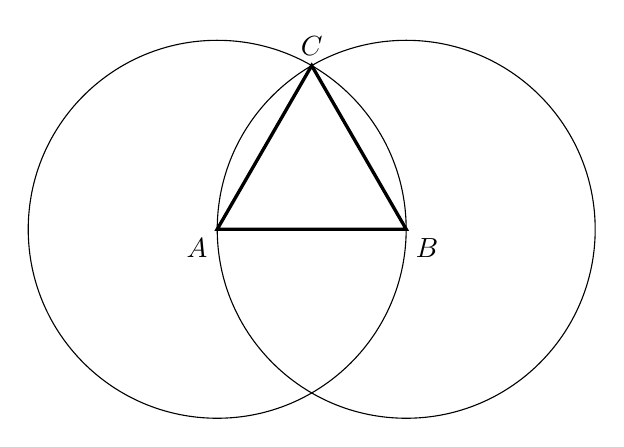
\begin{tikzpicture}[scale=1.2, line cap=round]
  \coordinate (A) at (0,0);
  \coordinate (B) at (2,0);
  \coordinate (C) at (1,{sqrt(3)});
  % Two circles, centres A and B, radius AB.
  \draw[thin] (A) circle (2);
  \draw[thin] (B) circle (2);
  % Triangle.
  \draw[very thick] (A) -- (B) -- (C) -- cycle;
  % Labels.
  \node[below left]  at (A) {$A$};
  \node[below right] at (B) {$B$};
  \node[above]       at (C) {$C$};
\end{tikzpicture}
\caption{Proposition I.1. The two circles with centres $A$ and $B$ and
common radius $AB$ meet at $C$; the triangle $ABC$ is equilateral.}
\label{fig:I.1}
\end{figure}

Let $AB$ be the given finite straight line.  With centre $A$ and
distance $AB$ describe the circle $BCD$ (Postulate 3).  With centre
$B$ and distance $BA$ describe the circle $ACE$ (Postulate 3).  From
the point $C$, where the circles cut one another, draw $CA$ and $CB$
(Postulate 1).  Since $A$ is the centre of $BCD$, $AC = AB$
(Definition I.15).  Since $B$ is the centre of $ACE$, $BC = BA$
(Definition I.15).  By Common Notion 1, $AC = BC$.  Therefore the
triangle $ABC$ is equilateral.
\dependson{I.1}{post:1}
\dependson{I.1}{post:3}
\dependson{I.1}{def:I.15}
\dependson{I.1}{cn:1}
\end{evidence}

\begin{claim}[Proposition I.2: Transfer a segment to a given point]
\label{prop:I.2}
To place at a given point (as an extremity) a straight line equal to a
given straight line.
\end{claim}
\begin{evidence}[Proof of I.2]
\label{ev:I.2}
Apply I.1 to obtain an equilateral triangle; produce its sides
(Postulate 2); describe a circle with centre at one endpoint of the
given segment cutting one of the produced sides; the cut-off equals
the given segment by Definition I.15 and Common Notion 1.
\dependson{I.2}{I.1}
\dependson{I.2}{post:1}
\dependson{I.2}{post:2}
\dependson{I.2}{post:3}
\dependson{I.2}{def:I.15}
\dependson{I.2}{cn:1}
\end{evidence}

\begin{claim}[Proposition I.3: Cut off a segment equal to a shorter]
\label{prop:I.3}
Given two unequal straight lines, to cut off from the greater a
straight line equal to the less.
\end{claim}
\begin{evidence}[Proof of I.3]
\label{ev:I.3}
Use I.2 to construct, at one extremity of the longer line, a segment
equal to the shorter.  Then by Definition I.15 the desired cut-off is
obtained.
\dependson{I.3}{I.2}
\dependson{I.3}{def:I.15}
\end{evidence}

\begin{claim}[Proposition I.4: SAS congruence]
\label{prop:I.4}
If two triangles have two sides equal to two sides respectively, and
have the angles contained by the equal straight lines equal, then they
will also have the base equal to the base, the triangle will be equal
to the triangle, and the remaining angles will be equal to the
remaining angles respectively.
\end{claim}
\begin{evidence}[Proof of I.4]
\label{ev:I.4}
Superpose one triangle on the other; corresponding sides and angles
coincide; by Common Notion 4 the figures are equal.
\dependson{I.4}{cn:4}
\end{evidence}

\begin{claim}[Proposition I.5: Pons asinorum]
\label{prop:I.5}
In isosceles triangles the angles at the base are equal to one
another; and if the equal straight lines be produced further, the
angles under the base will be equal to one another.
\end{claim}
\begin{evidence}[Proof of I.5]
\label{ev:I.5}
% fig-i-5.tex — I.5: pons asinorum (base angles of an isoceles triangle).
\begin{figure}[H]
\centering
\begin{tikzpicture}[scale=1.0, line cap=round]
  \coordinate (A) at (0, 3);
  \coordinate (B) at (-1.5, 0);
  \coordinate (C) at (1.5, 0);
  % Equal sides AB and AC, extended to F and G.
  \coordinate (F) at ($(A)!2.0!(B)$);
  \coordinate (G) at ($(A)!2.0!(C)$);
  \draw[thin]      (A) -- (F);
  \draw[thin]      (A) -- (G);
  \draw[very thick] (B) -- (C);
  % Points D on BF, E on CG with BD = CE.
  \coordinate (D) at ($(B)!0.5!(F)$);
  \coordinate (E) at ($(C)!0.5!(G)$);
  \draw[very thick, dashed] (B) -- (E);
  \draw[very thick, dashed] (C) -- (D);
  % Labels.
  \node[above]      at (A) {$A$};
  \node[left]       at (B) {$B$};
  \node[right]      at (C) {$C$};
  \node[below left] at (D) {$D$};
  \node[below right] at (E) {$E$};
  \node[below left] at (F) {$F$};
  \node[below right] at (G) {$G$};
\end{tikzpicture}
\caption{Proposition I.5. With $AB = AC$ and $BD = CE$ on the extensions,
triangles $ABE$ and $ACD$ are congruent (SAS, by I.4), whence the base
angles $\angle ABC = \angle ACB$.}
\label{fig:I.5}
\end{figure}

Apply I.3 to mark equal segments on the produced sides, then I.4 to
two pairs of congruent triangles.  Common Notion 3 gives equality of
the remaining angles.
\dependson{I.5}{I.3}
\dependson{I.5}{I.4}
\dependson{I.5}{cn:3}
\end{evidence}

\begin{claim}[Proposition I.6: Converse of I.5]
\label{prop:I.6}
If in a triangle two angles are equal to one another, the sides which
subtend the equal angles will also be equal to one another.
\end{claim}
\begin{evidence}[Proof of I.6]
\label{ev:I.6}
Suppose the sides unequal; cut off (by I.3) the greater equal to the
less; by I.4 the resulting smaller triangle equals the whole, which
contradicts Common Notion 5.  Therefore the sides are equal.
\dependson{I.6}{I.3}
\dependson{I.6}{I.4}
\dependson{I.6}{cn:5}
\end{evidence}

\begin{claim}[Proposition I.7: Uniqueness of triangle on a base]
\label{prop:I.7}
Given two straight lines constructed on a straight line and meeting in
a point, there cannot be constructed on the same straight line and on
the same side of it two other straight lines meeting in another point
and equal to the former two respectively, namely each to that which
has the same extremity with it.
\end{claim}
\begin{evidence}[Proof of I.7]
\label{ev:I.7}
A double application of I.5 yields contradictory angle equalities; by
Common Notion 5 the second meeting point cannot exist.
\dependson{I.7}{I.5}
\dependson{I.7}{cn:5}
\end{evidence}

\begin{claim}[Proposition I.8: SSS congruence]
\label{prop:I.8}
If two triangles have the two sides equal to two sides respectively,
and have also the base equal to the base, they will also have the
angles equal which are contained by the equal straight lines.
\end{claim}
\begin{evidence}[Proof of I.8]
\label{ev:I.8}
Superpose and apply I.7 to rule out a non-coincident image of the
contained angle; conclude by Common Notion 4.
\dependson{I.8}{I.7}
\dependson{I.8}{cn:4}
\end{evidence}

\begin{claim}[Proposition I.9: Angle bisection]
\label{prop:I.9}
To bisect a given rectilineal angle.
\end{claim}
\begin{evidence}[Proof of I.9]
\label{ev:I.9}
Apply I.1 to construct an equilateral triangle on a chord between the
angle's sides; the line from the vertex to the equilateral's apex
bisects the angle by I.8.
\dependson{I.9}{I.1}
\dependson{I.9}{I.8}
\end{evidence}

\begin{claim}[Proposition I.10: Segment bisection]
\label{prop:I.10}
To bisect a given finite straight line.
\end{claim}
\begin{evidence}[Proof of I.10]
\label{ev:I.10}
Apply I.1 to erect an equilateral triangle on the segment; bisect the
opposite angle by I.9; the bisector meets the segment at its midpoint
by I.4.
\dependson{I.10}{I.1}
\dependson{I.10}{I.9}
\dependson{I.10}{I.4}
\end{evidence}

\begin{claim}[Proposition I.11: Perpendicular at a point]
\label{prop:I.11}
To draw a straight line at right angles to a given straight line from
a given point on it.
\end{claim}
\begin{evidence}[Proof of I.11]
\label{ev:I.11}
Apply I.3 to mark equal segments either side of the given point, then
I.1 to erect an equilateral triangle whose apex line is perpendicular
(by I.8 and Definition I.10).
\dependson{I.11}{I.1}
\dependson{I.11}{I.3}
\dependson{I.11}{I.8}
\dependson{I.11}{def:I.10}
\end{evidence}

\begin{claim}[Proposition I.12: Perpendicular from external point]
\label{prop:I.12}
To draw a perpendicular straight line to a given infinite straight
line from a given point not on it.
\end{claim}
\begin{evidence}[Proof of I.12]
\label{ev:I.12}
With centre at the external point describe a circle (Postulate 3)
cutting the given line; bisect the chord by I.10; the line from the
external point to the midpoint is perpendicular by I.8.
\dependson{I.12}{I.8}
\dependson{I.12}{I.10}
\dependson{I.12}{post:3}
\end{evidence}

\begin{claim}[Proposition I.13: Adjacent angles sum to two right angles]
\label{prop:I.13}
If a straight line set up on a straight line make angles, it will
make either two right angles or angles equal to two right angles.
\end{claim}
\begin{evidence}[Proof of I.13]
\label{ev:I.13}
Drop a perpendicular by I.11; Common Notions 1--2 sum the resulting
two right angles to the unequal-case angle sum.
\dependson{I.13}{I.11}
\dependson{I.13}{cn:1}
\dependson{I.13}{cn:2}
\dependson{I.13}{def:I.10}
\end{evidence}

\begin{claim}[Proposition I.14: Converse of I.13]
\label{prop:I.14}
If with any straight line, and at a point on it, two straight lines
not lying on the same side make the adjacent angles equal to two
right angles, the two straight lines will be in a straight line with
one another.
\end{claim}
\begin{evidence}[Proof of I.14]
\label{ev:I.14}
Suppose not; then I.13 and Common Notion 1 yield contradictory angle
sums.
\dependson{I.14}{I.13}
\dependson{I.14}{cn:1}
\end{evidence}

\begin{claim}[Proposition I.15: Vertical angles]
\label{prop:I.15}
If two straight lines cut one another, they make the vertical angles
equal to one another.
\end{claim}
\begin{evidence}[Proof of I.15]
\label{ev:I.15}
Apply I.13 twice and Common Notion 3.
\dependson{I.15}{I.13}
\dependson{I.15}{cn:3}
\end{evidence}

\begin{claim}[Proposition I.16: Exterior angle of a triangle]
\label{prop:I.16}
In any triangle, if one of the sides be produced, the exterior angle
is greater than either of the interior and opposite angles.
\end{claim}
\begin{evidence}[Proof of I.16]
\label{ev:I.16}
Bisect a side by I.10; produce a median; apply I.4 to obtain a
congruent triangle that has the interior angle as one of its parts;
Common Notion 5 closes the inequality.
\dependson{I.16}{I.4}
\dependson{I.16}{I.10}
\dependson{I.16}{cn:5}
\end{evidence}

\begin{claim}[Proposition I.17: Sum of any two angles $<$ two right angles]
\label{prop:I.17}
In any triangle two angles taken together in any manner are less than
two right angles.
\end{claim}
\begin{evidence}[Proof of I.17]
\label{ev:I.17}
Apply I.16 and I.13.
\dependson{I.17}{I.13}
\dependson{I.17}{I.16}
\end{evidence}

\begin{claim}[Proposition I.18: Greater side subtends greater angle]
\label{prop:I.18}
In any triangle the greater side subtends the greater angle.
\end{claim}
\begin{evidence}[Proof of I.18]
\label{ev:I.18}
Cut off (I.3) a segment on the greater side equal to the lesser;
apply I.5 and I.16.
\dependson{I.18}{I.3}
\dependson{I.18}{I.5}
\dependson{I.18}{I.16}
\end{evidence}

\begin{claim}[Proposition I.19: Converse of I.18]
\label{prop:I.19}
In any triangle the greater angle is subtended by the greater side.
\end{claim}
\begin{evidence}[Proof of I.19]
\label{ev:I.19}
Suppose not; by I.5 and I.18 contradiction.
\dependson{I.19}{I.5}
\dependson{I.19}{I.18}
\end{evidence}

\begin{claim}[Proposition I.20: Triangle inequality]
\label{prop:I.20}
In any triangle two sides taken together in any manner are greater
than the remaining one.
\end{claim}
\begin{evidence}[Proof of I.20]
\label{ev:I.20}
Produce one side to an isosceles configuration by I.3; apply I.5 and
I.19.
\dependson{I.20}{I.3}
\dependson{I.20}{I.5}
\dependson{I.20}{I.19}
\end{evidence}

\begin{claim}[Proposition I.21: Interior cevian inequalities]
\label{prop:I.21}
If on one of the sides of a triangle, from its extremities, there be
constructed two straight lines meeting within the triangle, the
straight lines so constructed will be less than the remaining two
sides of the triangle, but will contain a greater angle.
\end{claim}
\begin{evidence}[Proof of I.21]
\label{ev:I.21}
Two applications of I.20 and one of I.16.
\dependson{I.21}{I.16}
\dependson{I.21}{I.20}
\end{evidence}

\begin{claim}[Proposition I.22: Triangle from three given segments]
\label{prop:I.22}
Out of three straight lines, which are equal to three given straight
lines, to construct a triangle: thus it is necessary that two of the
straight lines taken together in any manner should be greater than the
remaining one.
\end{claim}
\begin{evidence}[Proof of I.22]
\label{ev:I.22}
Apply I.20 (the necessity), then I.3 and Postulate 3 (the
construction).
\dependson{I.22}{I.3}
\dependson{I.22}{I.20}
\dependson{I.22}{post:3}
\end{evidence}

\begin{claim}[Proposition I.23: Reproduce a given angle]
\label{prop:I.23}
On a given straight line and at a point on it to construct a
rectilineal angle equal to a given rectilineal angle.
\end{claim}
\begin{evidence}[Proof of I.23]
\label{ev:I.23}
Cut equal segments by I.3, construct the matching triangle by I.22,
apply I.8.
\dependson{I.23}{I.3}
\dependson{I.23}{I.8}
\dependson{I.23}{I.22}
\end{evidence}

\begin{claim}[Proposition I.24: Hinge inequality]
\label{prop:I.24}
If two triangles have the two sides equal to two sides respectively,
but have the one of the angles contained by the equal straight lines
greater than the other, they will also have the base greater than the
base.
\end{claim}
\begin{evidence}[Proof of I.24]
\label{ev:I.24}
Apply I.23, I.4, I.5, and I.19.
\dependson{I.24}{I.4}
\dependson{I.24}{I.5}
\dependson{I.24}{I.19}
\dependson{I.24}{I.23}
\end{evidence}

\begin{claim}[Proposition I.25: Converse of I.24]
\label{prop:I.25}
If two triangles have the two sides equal to two sides respectively,
but have the one base greater than the other, they will also have the
one angle contained by the equal straight lines greater than the
other.
\end{claim}
\begin{evidence}[Proof of I.25]
\label{ev:I.25}
Suppose not and use I.4, I.24.
\dependson{I.25}{I.4}
\dependson{I.25}{I.24}
\end{evidence}

\begin{claim}[Proposition I.26: ASA / AAS congruence]
\label{prop:I.26}
If two triangles have the two angles equal to two angles respectively,
and one side equal to one side, namely either the side adjoining the
equal angles or that subtending one of the equal angles, they will
also have the remaining sides equal to the remaining sides and the
remaining angle equal to the remaining angle.
\end{claim}
\begin{evidence}[Proof of I.26]
\label{ev:I.26}
Apply I.4 to the congruent angle--side--angle case; for the AAS case
combine I.4 with I.16.
\dependson{I.26}{I.4}
\dependson{I.26}{I.16}
\end{evidence}

\begin{claim}[Proposition I.27: Alternate angles imply parallels]
\label{prop:I.27}
If a straight line falling on two straight lines make the alternate
angles equal to one another, the straight lines will be parallel to
one another.
\end{claim}
\begin{evidence}[Proof of I.27]
\label{ev:I.27}
Suppose the lines meet; I.16 gives a contradiction.  By Definition
I.23 they are parallel.
\dependson{I.27}{I.16}
\dependson{I.27}{def:I.23}
\end{evidence}

\begin{claim}[Proposition I.28: Corresponding angles imply parallels]
\label{prop:I.28}
If a straight line falling on two straight lines make the exterior
angle equal to the interior and opposite angle on the same side, or
the interior angles on the same side equal to two right angles, the
straight lines will be parallel to one another.
\end{claim}
\begin{evidence}[Proof of I.28]
\label{ev:I.28}
Reduce to I.27 via I.13 and I.15.
\dependson{I.28}{I.13}
\dependson{I.28}{I.15}
\dependson{I.28}{I.27}
\end{evidence}

\begin{claim}[Proposition I.29: Properties of parallels (uses Postulate 5)]
\label{prop:I.29}
A straight line falling on parallel straight lines makes the alternate
angles equal to one another, the exterior angle equal to the interior
and opposite angle, and the interior angles on the same side equal to
two right angles.
\end{claim}
\begin{evidence}[Proof of I.29]
\label{ev:I.29}
The first use of Postulate 5: any contrary supposition contradicts the
parallel postulate via I.13.
\dependson{I.29}{I.13}
\dependson{I.29}{post:5}
\end{evidence}

\begin{claim}[Proposition I.30: Transitivity of parallelism]
\label{prop:I.30}
Straight lines parallel to the same straight line are also parallel
to one another.
\end{claim}
\begin{evidence}[Proof of I.30]
\label{ev:I.30}
Two applications of I.29 and Common Notion 1.
\dependson{I.30}{I.29}
\dependson{I.30}{cn:1}
\end{evidence}

\begin{claim}[Proposition I.31: Construct a parallel through a point]
\label{prop:I.31}
Through a given point to draw a straight line parallel to a given
straight line.
\end{claim}
\begin{evidence}[Proof of I.31]
\label{ev:I.31}
Apply I.23 to reproduce the alternate angle at the given point and
I.27 to conclude parallelism.
\dependson{I.31}{I.23}
\dependson{I.31}{I.27}
\end{evidence}

\begin{claim}[Proposition I.32: Triangle angle sum]
\label{prop:I.32}
In any triangle, if one of the sides be produced, the exterior angle
is equal to the two interior and opposite angles, and the three
interior angles of the triangle are equal to two right angles.
\end{claim}
\begin{evidence}[Proof of I.32]
% fig-i-32.tex — I.32: triangle angle sum (parallel through apex).
\begin{figure}[H]
\centering
\begin{tikzpicture}[scale=1.2, line cap=round]
  \coordinate (A) at (-1.5, 0);
  \coordinate (B) at (2.0, 0);
  \coordinate (C) at (0.5, 2.4);
  \coordinate (D) at ($(C)!-1.4!(A)$); % line through C parallel to AB, on left
  \coordinate (E) at ($(C)!-1.4!(B)$); % line through C parallel to AB, on right
  % Triangle.
  \draw[very thick] (A) -- (B) -- (C) -- cycle;
  % Parallel through C, drawn long.
  \draw[thin] ($(C)!-0.7!(B)$) -- ($(C)!1.5!(B)$);
  % Side AB extended beyond B to F to expose exterior angle.
  \coordinate (F) at ($(A)!1.4!(B)$);
  \draw[thin] (B) -- (F);
  % Labels.
  \node[below left]  at (A) {$A$};
  \node[below right] at (B) {$B$};
  \node[above]       at (C) {$C$};
  \node[below right] at (F) {$F$};
  \node[above left]  at ($(C)!-0.7!(B)$) {$D$};
  \node[above right] at ($(C)!1.5!(B)$) {$E$};
\end{tikzpicture}
\caption{Proposition I.32. Drawing $DE$ through $C$ parallel to $AB$
makes $\angle DCA = \angle CAB$ (alternate, I.29) and $\angle ECB =
\angle ABC$ (alternate, I.29); the straight angle at $C$ then sums
the three interior angles of $\triangle ABC$ to two right angles.}
\label{fig:I.32}
\end{figure}

\label{ev:I.32}
Apply I.31 to draw a parallel through the apex; apply I.29 twice and
Common Notion 2.
\dependson{I.32}{I.29}
\dependson{I.32}{I.31}
\dependson{I.32}{cn:2}
\end{evidence}

\begin{claim}[Proposition I.33: Connecting equal-and-parallel pairs]
\label{prop:I.33}
The straight lines joining equal and parallel straight lines (at the
extremities which are in the same directions) are themselves equal
and parallel.
\end{claim}
\begin{evidence}[Proof of I.33]
\label{ev:I.33}
Apply I.4 to the resulting two triangles and I.29 + I.27 for
parallelism.
\dependson{I.33}{I.4}
\dependson{I.33}{I.27}
\dependson{I.33}{I.29}
\end{evidence}

\begin{claim}[Proposition I.34: Properties of parallelograms]
\label{prop:I.34}
In parallelogrammic areas the opposite sides and angles are equal to
one another, and the diameter bisects the areas.
\end{claim}
\begin{evidence}[Proof of I.34]
\label{ev:I.34}
Apply I.29 and I.26 to the two triangles cut by the diameter, then
Common Notion 2.
\dependson{I.34}{I.26}
\dependson{I.34}{I.29}
\dependson{I.34}{cn:2}
\end{evidence}

\begin{claim}[Proposition I.35: Parallelograms with same base \& between same parallels]
\label{prop:I.35}
Parallelograms which are on the same base and in the same parallels
are equal to one another.
\end{claim}
\begin{evidence}[Proof of I.35]
\label{ev:I.35}
Apply I.34 and I.4 to congruent triangles; conclude by Common Notions
2--3.
\dependson{I.35}{I.4}
\dependson{I.35}{I.34}
\dependson{I.35}{cn:2}
\dependson{I.35}{cn:3}
\end{evidence}

\begin{claim}[Proposition I.36: Parallelograms with equal bases]
\label{prop:I.36}
Parallelograms which are on equal bases and in the same parallels are
equal to one another.
\end{claim}
\begin{evidence}[Proof of I.36]
\label{ev:I.36}
Translate one parallelogram via I.33 to share a base with the other,
then apply I.35.
\dependson{I.36}{I.33}
\dependson{I.36}{I.35}
\end{evidence}

\begin{claim}[Proposition I.37: Triangles with same base \& parallels]
\label{prop:I.37}
Triangles which are on the same base and in the same parallels are
equal to one another.
\end{claim}
\begin{evidence}[Proof of I.37]
\label{ev:I.37}
Complete each triangle to a parallelogram via I.31, then apply I.34
and I.35.
\dependson{I.37}{I.31}
\dependson{I.37}{I.34}
\dependson{I.37}{I.35}
\end{evidence}

\begin{claim}[Proposition I.38: Triangles with equal bases]
\label{prop:I.38}
Triangles which are on equal bases and in the same parallels are
equal to one another.
\end{claim}
\begin{evidence}[Proof of I.38]
\label{ev:I.38}
Same construction as I.37 with I.36 in place of I.35.
\dependson{I.38}{I.31}
\dependson{I.38}{I.34}
\dependson{I.38}{I.36}
\end{evidence}

\begin{claim}[Proposition I.39: Equal triangles on same base $\Rightarrow$ same parallels]
\label{prop:I.39}
Equal triangles which are on the same base and on the same side are
also in the same parallels.
\end{claim}
\begin{evidence}[Proof of I.39]
\label{ev:I.39}
Apply I.31 to draw a parallel; I.37 forces the second vertex onto it.
\dependson{I.39}{I.31}
\dependson{I.39}{I.37}
\end{evidence}

\begin{claim}[Proposition I.40: Equal triangles on equal bases]
\label{prop:I.40}
Equal triangles which are on equal bases and on the same side are
also in the same parallels.
\end{claim}
\begin{evidence}[Proof of I.40]
\label{ev:I.40}
Same approach as I.39 with I.38 in place of I.37.
\dependson{I.40}{I.31}
\dependson{I.40}{I.38}
\end{evidence}

\begin{claim}[Proposition I.41: Parallelogram is double a triangle]
\label{prop:I.41}
If a parallelogram have the same base with a triangle and be in the
same parallels, the parallelogram is double of the triangle.
\end{claim}
\begin{evidence}[Proof of I.41]
\label{ev:I.41}
Apply I.34 and I.37; double via Common Notion 2.
\dependson{I.41}{I.34}
\dependson{I.41}{I.37}
\dependson{I.41}{cn:2}
\end{evidence}

\begin{claim}[Proposition I.42: Construct a parallelogram equal in area to a triangle]
\label{prop:I.42}
To construct, in a given rectilineal angle, a parallelogram equal to
a given triangle.
\end{claim}
\begin{evidence}[Proof of I.42]
\label{ev:I.42}
Bisect a side by I.10; apply I.23 to set the angle; apply I.31 and
I.41.
\dependson{I.42}{I.10}
\dependson{I.42}{I.23}
\dependson{I.42}{I.31}
\dependson{I.42}{I.41}
\end{evidence}

\begin{claim}[Proposition I.43: Complements of a parallelogram]
\label{prop:I.43}
In any parallelogram the complements of the parallelograms about the
diameter are equal to one another.
\end{claim}
\begin{evidence}[Proof of I.43]
\label{ev:I.43}
Apply I.34 to the bisecting diameter and Common Notions 2--3.
\dependson{I.43}{I.34}
\dependson{I.43}{cn:2}
\dependson{I.43}{cn:3}
\end{evidence}

\begin{claim}[Proposition I.44: Apply a parallelogram to a segment equal to a triangle]
\label{prop:I.44}
To a given straight line to apply, in a given rectilineal angle, a
parallelogram equal to a given triangle.
\end{claim}
\begin{evidence}[Proof of I.44]
\label{ev:I.44}
Apply I.42 and I.43 in sequence.
\dependson{I.44}{I.42}
\dependson{I.44}{I.43}
\end{evidence}

\begin{claim}[Proposition I.45: Apply a parallelogram equal to a rectilineal figure]
\label{prop:I.45}
To construct, in a given rectilineal angle, a parallelogram equal to
a given rectilineal figure.
\end{claim}
\begin{evidence}[Proof of I.45]
\label{ev:I.45}
Triangulate the figure; sum the parallelograms by repeated I.44 and
Common Notion 2.
\dependson{I.45}{I.44}
\dependson{I.45}{cn:2}
\end{evidence}

\begin{claim}[Proposition I.46: Construct a square on a segment]
\label{prop:I.46}
On a given straight line to describe a square.
\end{claim}
\begin{evidence}[Proof of I.46]
\label{ev:I.46}
Apply I.11 to erect perpendiculars; use I.3 to cut off equal segments;
use I.31 and I.29 to close the square; verify right angles via I.34.
\dependson{I.46}{I.3}
\dependson{I.46}{I.11}
\dependson{I.46}{I.29}
\dependson{I.46}{I.31}
\dependson{I.46}{I.34}
\end{evidence}

\begin{claim}[Proposition I.47: Pythagoras' theorem]
\label{prop:I.47}
In right-angled triangles the square on the side subtending the right
angle is equal to the squares on the sides containing the right angle.
\end{claim}
\begin{evidence}[Proof of I.47]
% fig-i-47.tex — I.47: Pythagoras (square decomposition).
\begin{figure}[H]
\centering
\begin{tikzpicture}[scale=0.55, line cap=round, line join=round]
  % Right triangle vertices: right angle at A.
  \coordinate (A) at (0, 0);
  \coordinate (B) at (3, 0); % horizontal leg
  \coordinate (C) at (0, 4); % vertical leg
  % Hypotenuse BC.
  % Square on AB (below): A, B, B', A'
  \coordinate (Ap) at (0, -3);
  \coordinate (Bp) at (3, -3);
  % Square on AC (left): A, C, C', A''
  \coordinate (App) at (-4, 0);
  \coordinate (Cp)  at (-4, 4);
  % Square on BC (outward): B, C, C'', B''
  % Outward direction = rotate (B-C) by -90.
  \coordinate (Bpp) at ($(B)!1!-90:(C)$);
  \coordinate (Cpp) at ($(C)!1!90:(B)$);
  % Triangle.
  \draw[very thick] (A) -- (B) -- (C) -- cycle;
  % Three squares.
  \draw[thick, fill=gray!10] (A)   -- (B)   -- (Bp)  -- (Ap)  -- cycle;
  \draw[thick, fill=gray!10] (A)   -- (C)   -- (Cp)  -- (App) -- cycle;
  \draw[thick, fill=gray!20] (B)   -- (C)   -- (Cpp) -- (Bpp) -- cycle;
  % Altitude from A to BC, foot at H, extended to meet square on BC.
  \coordinate (H) at ($(B)!(A)!(C)$);
  \coordinate (Hext) at ($(H)!1!-90:(B)$);
  \draw[thin, dashed] (A) -- (Hext);
  % Labels.
  \node[below right]      at (A) {$A$};
  \node[below]            at (B) {$B$};
  \node[left]             at (C) {$C$};
  \node[left]             at ($(A)!0.5!(App)$) {square on $AC$};
  \node                   at ($(A)!0.5!(Bp)+(0.5,-1.5)$) {square on $AB$};
  \node                   at ($(B)!0.5!(Cpp)+(1.7,0.7)$) {square on $BC$};
\end{tikzpicture}
\caption{Proposition I.47. The square on the hypotenuse $BC$ is
partitioned by the altitude $AH$ extended into two rectangles, each
equal (by I.41 + I.46) to a square on a leg; thus $BC^2 = AB^2 + AC^2$.}
\label{fig:I.47}
\end{figure}

\label{ev:I.47}
Erect squares on each side via I.46; using I.14, I.31 and I.41 show
each part-square equals a corresponding parallelogram cut off the
hypotenuse-square by the perpendicular from the right angle; sum via
Common Notion 2.
\dependson{I.47}{I.4}
\dependson{I.47}{I.14}
\dependson{I.47}{I.31}
\dependson{I.47}{I.41}
\dependson{I.47}{I.46}
\dependson{I.47}{cn:2}
\supports{I.47}{I.48}
\end{evidence}

\begin{claim}[Proposition I.48: Converse of Pythagoras]
\label{prop:I.48}
If in a triangle the square on one of the sides be equal to the
squares on the remaining two sides of the triangle, the angle
contained by the remaining two sides of the triangle is right.
\end{claim}
\begin{evidence}[Proof of I.48]
\label{ev:I.48}
Construct a right triangle with the same two legs by I.11; apply
I.47, I.8, and Common Notion 1.
\dependson{I.48}{I.8}
\dependson{I.48}{I.11}
\dependson{I.48}{I.47}
\dependson{I.48}{cn:1}
\end{evidence}

% book02.tex — Book II: Geometric algebra. Scaffolded.

\section{Book II --- Geometric Algebra}
\label{sec:book-II}

Book II contains the famous identities of geometric algebra, including
the distributivity of multiplication over addition (II.1) and the
law of cosines in its purely-geometric form (II.12, II.13). Definitions
introduce the gnomon construction used throughout.

\begin{claim}[Proposition II.1: Distributivity of multiplication]
\label{prop:II.1}
If there be two straight lines, and one of them be cut into any
number of segments whatever, the rectangle contained by the two
straight lines is equal to the rectangles contained by the
uncut straight line and each of the segments.
\end{claim}
\begin{evidence}[Proof sketch of II.1]
\label{ev:II.1}
Construction follows Heath. To be filled in fully in a later version.
\dependson{II.1}{I.31}
\dependson{II.1}{I.34}
\dependson{II.1}{cn:2}
\end{evidence}

\begin{claim}[Proposition II.12: Obtuse-triangle generalisation of Pythagoras]
\label{prop:II.12}
In obtuse-angled triangles the square on the side subtending the
obtuse angle is greater than the squares on the sides containing the
obtuse angle by twice the rectangle contained by one of the sides
about the obtuse angle (namely that on which the perpendicular falls)
and the straight line cut off outside by the perpendicular.
\end{claim}
\begin{evidence}[Proof sketch of II.12]
\label{ev:II.12}
Apply II.4 (square of a sum) and I.47.  To be filled in fully.
\dependson{II.12}{I.47}
\end{evidence}

% TODO: Propositions II.2 through II.14 (excluding II.12) — translations
% follow Heath; dependency edges to be added per the rrxiv convention.

% book03.tex --- Book III of Euclid's Elements: Circles.
%
% All 37 propositions encoded with Heath-faithful statements and
% proof sketches; \dependson edges thread back to Book I (chiefly I.4,
% I.5, I.8, I.11, I.12, I.16, I.20, I.23, I.32, I.47) and Book II
% (II.5, II.6 for the power-of-a-point group).
%
% Wording follows Heath (1908); proof prose mirrors his density.

\section{Book III --- Circles}
\label{sec:book-III}

\begin{claim}[Proposition III.1: To find the centre of a given circle]
\label{prop:III.1}
To find the centre of a given circle.
\end{claim}
\begin{evidence}[Proof of III.1]
\label{ev:III.1}
Let $ABC$ be the given circle.  Draw any chord $AB$ in it (Postulate
1) and bisect $AB$ at $D$ (I.10).  From $D$ draw $DC$ at right
angles to $AB$ (I.11), produced to meet the circle at $C$ and $E$.
Bisect $CE$ at $F$ (I.10); then $F$ is the centre.  For if any other
point $G$ were the centre, then by SSS (I.8) on $\triangle GAD$ and
$\triangle GBD$ we would obtain $\angle GDA = \angle GDB$, both
right (I.13).  But $F$ already lies on the perpendicular bisector
of $AB$, and the perpendicular at $D$ is unique (I.11); applying
the same reasoning to chord $CE$ forces $F$ onto its perpendicular
bisector as well.  The two perpendicular bisectors meet only at the
true centre, which is $F$.
\dependson{III.1}{I.8}
\dependson{III.1}{I.10}
\dependson{III.1}{I.11}
\dependson{III.1}{I.13}
\dependson{III.1}{post:1}
\dependson{III.1}{def:I.15}
\end{evidence}

\begin{claim}[Proposition III.2: A chord lies inside the circle]
\label{prop:III.2}
If on the circumference of a circle two points be taken at random,
the straight line joining the points will fall within the circle.
\end{claim}
\begin{evidence}[Proof of III.2]
\label{ev:III.2}
Let $A$, $B$ be on the circle with centre $E$ (III.1).  Suppose for
contradiction that some point $F$ on the chord $AB$ lies outside the
circle; then $EF > EA$.  Join $EA$, $EB$.  By I.5, the base angles
of the isoceles $\triangle EAB$ are equal: $\angle EAB = \angle
EBA$.  By I.16, the exterior angle at any interior point $F$ of
$AB$ is greater than either remote interior angle; pursuing the
inequalities (Heath's argument) forces $EF < EA$ for $F$ inside
$AB$, contradicting the assumption.  Hence every point of $AB$ lies
within the circle.
\dependson{III.2}{III.1}
\dependson{III.2}{I.5}
\dependson{III.2}{I.16}
\dependson{III.2}{def:I.15}
\end{evidence}

\begin{claim}[Proposition III.3: Centre-line bisects chord iff perpendicular]
\label{prop:III.3}
If in a circle a straight line through the centre bisect a straight
line not through the centre, it also cuts it at right angles; and if
it cut it at right angles, it also bisects it.
\end{claim}
\begin{evidence}[Proof of III.3]
\label{ev:III.3}
Let $AB$ be a chord not through the centre $E$, and $CD$ a line
through $E$ meeting $AB$ at $F$.  Suppose $CD$ bisects $AB$, so
$AF = FB$.  Join $EA$, $EB$.  In $\triangle EAF$ and $\triangle
EBF$: $EA = EB$ (radii), $AF = FB$ (given), $EF$ common.  By I.8 the
triangles are congruent, so $\angle EFA = \angle EFB$, and by I.13
both are right.  Conversely, if $CD \perp AB$ at $F$, then in the
right triangles $\triangle EAF$ and $\triangle EBF$ we have $EA =
EB$ and $EF$ common, with right angles at $F$; by I.4 (SAS variant)
or I.26 (ASA), $AF = FB$.
\dependson{III.3}{III.1}
\dependson{III.3}{I.4}
\dependson{III.3}{I.8}
\dependson{III.3}{I.13}
\dependson{III.3}{I.26}
\dependson{III.3}{def:I.15}
\end{evidence}

\begin{claim}[Proposition III.4: Two non-diameter chords cannot bisect each other]
\label{prop:III.4}
If in a circle two straight lines cut one another which are not
through the centre, they do not bisect one another.
\end{claim}
\begin{evidence}[Proof of III.4]
\label{ev:III.4}
Let $AB$, $CD$ be two chords intersecting at $E$, neither through
the centre $F$.  Suppose for contradiction that $E$ bisects both:
$AE = EB$ and $CE = ED$.  Join $FE$.  By III.3 applied to chord
$AB$ (since $F$ is the centre and $FE$ bisects $AB$ at $E$), $FE
\perp AB$.  Applied to $CD$, the same line $FE$ is $\perp CD$.  But
the perpendicular from $F$ to a line is unique (I.11), so $AB$ and
$CD$ must coincide --- contradiction with their being two distinct
chords.
\dependson{III.4}{III.3}
\dependson{III.4}{I.11}
\dependson{III.4}{cn:1}
\end{evidence}

\begin{claim}[Proposition III.5: Two intersecting circles have distinct centres]
\label{prop:III.5}
If two circles cut one another, they will not have the same centre.
\end{claim}
\begin{evidence}[Proof of III.5]
\label{ev:III.5}
Let circles $\Gamma_1$ and $\Gamma_2$ meet at points $A$ and $B$.
Suppose they share centre $E$.  Then $EA$ is a radius of $\Gamma_1$
and also of $\Gamma_2$; the two circles thus have the same centre
and the same radius, so they coincide --- contradicting their
meeting at only two points (or in general, being two distinct
circles).
\dependson{III.5}{def:I.15}
\dependson{III.5}{def:III.1}
\end{evidence}

\begin{claim}[Proposition III.6: Tangent circles have distinct centres]
\label{prop:III.6}
If two circles touch one another, they will not have the same centre.
\end{claim}
\begin{evidence}[Proof of III.6]
\label{ev:III.6}
By the same argument as III.5: a shared centre and a common point on
the circumference of both circles force equal radii, hence coincident
circles.
\dependson{III.6}{III.5}
\dependson{III.6}{def:I.15}
\dependson{III.6}{def:III.3}
\end{evidence}

\begin{claim}[Proposition III.7: Distances from an interior non-centre point]
\label{prop:III.7}
If on the diameter of a circle a point be taken which is not the
centre, and from the point straight lines fall upon the circle: that
will be greatest on which the centre is, the remainder of the same
diameter will be least, and of the rest the nearer to the diameter
through the centre is always greater than the more remote.
\end{claim}
\begin{evidence}[Proof of III.7]
\label{ev:III.7}
Let $AD$ be a diameter of circle $ABCD$ with centre $E$, and let
$F$ on $AD$ be distinct from $E$.  From $F$ draw lines $FB$, $FC$
to the circumference.  Join $EB$, $EC$.

In $\triangle EBF$: $EB + EF > FB$ (I.20).  But $EB = EA$ (radii)
and $EF + EA = FA$, so $FA = EF + EB > FB$; hence the line $FA$
along the diameter towards the centre is longer than any other.
The line $FD$ on the other side is similarly the shortest.  For
intermediate lines $FB$ vs $FC$ with $B$ closer to $A$ than $C$,
the SAS inequality I.24 in the radius-line-radius triangles gives
$FB > FC$ when $\angle BEF > \angle CEF$.
\dependson{III.7}{I.5}
\dependson{III.7}{I.20}
\dependson{III.7}{I.24}
\dependson{III.7}{def:I.15}
\end{evidence}

\begin{claim}[Proposition III.8: Distances from an exterior point]
\label{prop:III.8}
If a point be taken outside a circle and from the point straight
lines be drawn through to the circle, one of which is through the
centre and the others fall on the circle: of the lines falling on
the concave circumference, that through the centre is greatest, and
the nearer to it always greater than the more remote; and of those
falling on the convex circumference, that between the point and the
diameter is least, and the nearer to it always less than the more
remote.
\end{claim}
\begin{evidence}[Proof of III.8]
\label{ev:III.8}
The argument mirrors III.7 with the point outside.  Let $D$ be the
external point and $AD$ the line through $D$ and the centre $E$,
meeting the circle at $A$ (near) and $C$ (far).  For any other line
from $D$ meeting the circle at $G$ (near) and $K$ (far), I.20 gives
$DG + GE > DE$, and the SAS inequality I.24 again orders the
distances by the angles at $E$.  The "two lengths per secant"
ordering (concave/convex) follows by separating the near and far
intersections.
\dependson{III.8}{III.7}
\dependson{III.8}{I.20}
\dependson{III.8}{I.24}
\dependson{III.8}{def:I.15}
\end{evidence}

\begin{claim}[Proposition III.9: Three equal interior distances force the centre]
\label{prop:III.9}
If a point be taken within a circle, and more than two equal
straight lines fall from the point on the circle, the point taken is
the centre of the circle.
\end{claim}
\begin{evidence}[Proof of III.9]
\label{ev:III.9}
Let $F$ be the point and $FA$, $FB$, $FC$ three equal lines to the
circle.  Join $AB$, $BC$; bisect them at $G$, $H$ (I.10).  Join
$FG$, $FH$.  In $\triangle FAG$ and $\triangle FBG$: $FA = FB$ given,
$AG = GB$ by construction, $FG$ common; by I.8 the triangles are
congruent, so $\angle FGA = \angle FGB$, and by I.13 both are right.
Similarly $FH \perp BC$.  By III.3 (rewriting it as: the
perpendicular at the midpoint of a chord passes through the centre),
both $FG$ produced and $FH$ produced pass through the centre.  Their
intersection $F$ is therefore the centre.
\dependson{III.9}{III.1}
\dependson{III.9}{III.3}
\dependson{III.9}{I.8}
\dependson{III.9}{I.10}
\dependson{III.9}{I.13}
\dependson{III.9}{def:I.15}
\end{evidence}

\begin{claim}[Proposition III.10: Two circles meet in at most two points]
\label{prop:III.10}
A circle does not cut a circle at more points than two.
\end{claim}
\begin{evidence}[Proof of III.10]
\label{ev:III.10}
Suppose two circles meet at three points $A$, $B$, $C$.  By III.9,
the centre of each circle is the unique point equidistant from any
three points on its circumference --- so both circles have the same
centre.  Then by III.5 they coincide, contradicting their being two
distinct circles.
\dependson{III.10}{III.5}
\dependson{III.10}{III.9}
\end{evidence}

\begin{claim}[Proposition III.11: Internal tangent: line of centres passes through contact]
\label{prop:III.11}
If two circles touch one another internally, and their centres be
taken, the straight line joining their centres, if produced, will
fall on the point of contact of the circles.
\end{claim}
\begin{evidence}[Proof of III.11]
\label{ev:III.11}
Let circle $\Gamma_1$ contain circle $\Gamma_2$, touching at $A$,
with centres $F$ (of $\Gamma_1$) and $G$ (of $\Gamma_2$).  Suppose
the line $FG$ produced does not pass through $A$.  Join $FA$, $GA$.
In $\triangle FAG$: by the triangle inequality (I.20), $FA + AG >
FG$.  Produce $FG$ to meet $\Gamma_1$ at $H$ and $\Gamma_2$ at $K$.
Then $FA = FH$ (radii of $\Gamma_1$), $GA = GK$ (radii of
$\Gamma_2$), and $H$ lies beyond $K$ on segment $FG$ extended.  So
$FA + AG = FH + GK = FG + (HK > 0)$, i.e.\ $FA + AG > FG$ ---
consistent.  But $\Gamma_2$ is internally tangent, so $H = K$, and
$FA + AG = FG$, contradicting the strict inequality.  Hence $A$
lies on line $FG$.
\dependson{III.11}{I.20}
\dependson{III.11}{def:I.15}
\dependson{III.11}{def:III.3}
\end{evidence}

\begin{claim}[Proposition III.12: External tangent: line of centres passes through contact]
\label{prop:III.12}
If two circles touch one another externally, the straight line
joining their centres will pass through the point of contact.
\end{claim}
\begin{evidence}[Proof of III.12]
\label{ev:III.12}
Analogous to III.11.  For externally tangent circles, the point of
contact $A$ lies on the segment $FG$ between the centres, and
$FA + AG = FG$ exactly.  The triangle inequality I.20 then forces
$A$ to lie on the line $FG$.
\dependson{III.12}{III.11}
\dependson{III.12}{I.20}
\dependson{III.12}{def:III.3}
\end{evidence}

\begin{claim}[Proposition III.13: Tangent circles meet in at most one point]
\label{prop:III.13}
A circle does not touch a circle at more points than one, whether it
touch it internally or externally.
\end{claim}
\begin{evidence}[Proof of III.13]
\label{ev:III.13}
Suppose two circles touch at two points $A$, $B$.  By III.11
(internal) or III.12 (external), both $A$ and $B$ lie on the line
joining the centres.  Thus this line cuts each circle in two
points, making it a diameter of each.  But then $AB$ is a chord of
each circle equal in length to the diameter --- so $A$ and $B$ are
antipodal points on each circle, and both circles share centre and
diameter, contradicting III.5/III.6.
\dependson{III.13}{III.5}
\dependson{III.13}{III.6}
\dependson{III.13}{III.11}
\dependson{III.13}{III.12}
\end{evidence}

\begin{claim}[Proposition III.14: Equal chords are equidistant from the centre]
\label{prop:III.14}
In a circle equal straight lines are equally distant from the centre,
and those which are equally distant from the centre are equal to one
another.
\end{claim}
\begin{evidence}[Proof of III.14]
\label{ev:III.14}
Let $AB$ and $CD$ be chords with $AB = CD$.  From the centre $E$
drop perpendiculars $EF$ to $AB$ and $EG$ to $CD$ (I.12).  By III.3,
$AF = FB = AB/2$ and $CG = GD = CD/2$, so $AF = CG$.  Join $EA$,
$EC$ (both radii, so equal).  In right triangles $\triangle EAF$
and $\triangle ECG$ (right angles at $F$, $G$), I.47 gives $EA^2 =
AF^2 + EF^2$ and $EC^2 = CG^2 + EG^2$.  Subtracting (Common Notion
3) and using $EA = EC$, $AF = CG$ gives $EF^2 = EG^2$, hence $EF =
EG$.  Conversely, if $EF = EG$, the same I.47 identity gives $AF =
CG$ and hence $AB = CD$.
\dependson{III.14}{III.3}
\dependson{III.14}{I.12}
\dependson{III.14}{I.47}
\dependson{III.14}{cn:3}
\dependson{III.14}{def:III.4}
\end{evidence}

\begin{claim}[Proposition III.15: Diameter is the longest chord]
\label{prop:III.15}
Of straight lines in a circle the diameter is greatest, and of the
rest the nearer to the centre is always greater than the more remote.
\end{claim}
\begin{evidence}[Proof of III.15]
\label{ev:III.15}
Let $AD$ be a diameter, and $BC$ any other chord.  From the centre
$E$ drop $EF \perp BC$ (I.12).  By III.3, $F$ is the midpoint of
$BC$, so $BF = BC/2$.  By I.47 in $\triangle EBF$: $EB^2 = BF^2 +
EF^2$.  Since $EB = $ radius $= AD/2$, $(AD/2)^2 = (BC/2)^2 +
EF^2$, hence $BC^2 = AD^2 - 4\cdot EF^2 < AD^2$ when $EF > 0$.  So
the diameter $AD$ is the longest chord.  For two non-diameter
chords with distances $EF_1 < EF_2$ from the centre, the same
identity gives the chord through $F_1$ longer than the one through
$F_2$.
\dependson{III.15}{III.3}
\dependson{III.15}{I.12}
\dependson{III.15}{I.47}
\dependson{III.15}{def:III.4}
\dependson{III.15}{def:III.5}
\end{evidence}

\begin{claim}[Proposition III.16: Perpendicular at diameter endpoint is tangent]
\label{prop:III.16}
The straight line drawn at right angles to the diameter of a circle
from its extremity will fall outside the circle, and into the space
between the straight line and the circumference another straight
line cannot be interposed.
\end{claim}
\begin{evidence}[Proof of III.16]
\label{ev:III.16}
Let $AB$ be a diameter and $AC$ drawn at right angles to $AB$ at
$A$ (I.11).  Suppose $AC$ meets the circle at another point $D
\neq A$; join $BD$.  Since $AB$ is a diameter and $D$ on the
circle, by III.31 (proved independently below) $\angle ADB$ is
right.  But $\angle DAB$ is also right by construction; the sum of
two angles of $\triangle ABD$ is then two right angles, leaving no
positive angle at $B$ --- contradicting I.17.  Hence $AC$ meets the
circle only at $A$.  The "no other line interposable" follows from
the uniqueness of the perpendicular (I.11): any line through $A$
not perpendicular to $AB$ makes a non-right angle and cuts the
circle.
\dependson{III.16}{I.11}
\dependson{III.16}{I.17}
\dependson{III.16}{I.32}
\dependson{III.16}{III.31}
\dependson{III.16}{def:III.2}
\end{evidence}

\begin{claim}[Proposition III.17: Tangent from an external point]
\label{prop:III.17}
From a given point to draw a straight line touching a given circle.
\end{claim}
\begin{evidence}[Proof of III.17]
\label{ev:III.17}
Let $A$ be the external point and $BCD$ the circle with centre $E$.
Join $AE$, and at $E$ erect a perpendicular to $AE$ (I.11); with
$E$ as centre and $EA$ as radius describe a circle $AFG$, meeting
the perpendicular at $F$.  Join $FA$, meeting the original circle
$BCD$ at $B$.  Then $AB$ is the desired tangent.

Proof: $\triangle ABE$ and $\triangle AFE$ are congruent by SAS
($EA$ common, $EB = EF$ both equal to the radius of $AFG$,
$\angle AEB = \angle AEF$ by construction); hence $\angle ABE =
\angle AFE$, which is right.  So $AB \perp EB$, the radius at the
point of contact, and by III.18 (next) $AB$ is tangent.
\dependson{III.17}{III.1}
\dependson{III.17}{III.16}
\dependson{III.17}{I.4}
\dependson{III.17}{I.11}
\dependson{III.17}{def:I.15}
\end{evidence}

\begin{claim}[Proposition III.18: Tangent is perpendicular to the radius at contact]
\label{prop:III.18}
If a straight line touch a circle, and a straight line be joined
from the centre to the point of contact, the straight line so joined
will be perpendicular to the tangent.
\end{claim}
\begin{evidence}[Proof of III.18]
\label{ev:III.18}
Let line $AB$ touch the circle at $C$, with centre $F$.  Suppose $FC$
is not perpendicular to $AB$; drop the perpendicular $FG$ to $AB$
at some point $G \neq C$.  In right triangle $\triangle FGC$
(right-angled at $G$), $FC$ is the hypotenuse, so by I.19, $FG <
FC$.  But $G$ lies on the tangent $AB$, which has no point inside
the circle (Definition III.2); so $FG \geq FC = $ radius.  The two
inequalities contradict.  Hence $G = C$ and $FC \perp AB$.
\dependson{III.18}{I.11}
\dependson{III.18}{I.19}
\dependson{III.18}{def:III.2}
\dependson{III.18}{def:I.15}
\end{evidence}

\begin{claim}[Proposition III.19: Centre lies on the perpendicular to the tangent]
\label{prop:III.19}
If a straight line touch a circle, and from the point of contact a
straight line be drawn at right angles to the tangent, the centre of
the circle will be on the straight line so drawn.
\end{claim}
\begin{evidence}[Proof of III.19]
\label{ev:III.19}
By III.18, the line from the centre to the contact point is
perpendicular to the tangent.  Conversely, the perpendicular at the
contact point in the plane is unique (I.11), so the centre must lie
on it.  (If the centre were off this perpendicular, the line from
centre to contact would not be perpendicular to the tangent,
contradicting III.18.)
\dependson{III.19}{III.18}
\dependson{III.19}{I.11}
\dependson{III.19}{def:III.2}
\end{evidence}

\begin{claim}[Proposition III.20: Inscribed angle is half the central angle]
\label{prop:III.20}
In a circle the angle at the centre is double of the angle at the
circumference, when the angles have the same circumference as base.
\end{claim}
\begin{evidence}[Proof of III.20]
\label{ev:III.20}
% fig-iii-20.tex — III.20: inscribed angle theorem.
\begin{figure}[H]
\centering
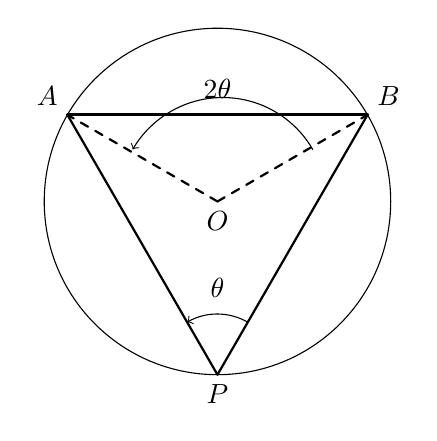
\begin{tikzpicture}[scale=1.1, line cap=round]
  \coordinate (O) at (0, 0);
  \def\r{2}
  \draw[thin] (O) circle (\r);
  \coordinate (A) at ({\r*cos(150)}, {\r*sin(150)}); % on circle, left
  \coordinate (B) at ({\r*cos(30)},  {\r*sin(30)});  % on circle, right
  \coordinate (P) at ({\r*cos(270)}, {\r*sin(270)}); % on circle, bottom (point opposite arc)
  % Chord AB.
  \draw[very thick] (A) -- (B);
  % Inscribed angle from P.
  \draw[thick] (P) -- (A);
  \draw[thick] (P) -- (B);
  % Central angle from O.
  \draw[thick, dashed] (O) -- (A);
  \draw[thick, dashed] (O) -- (B);
  \node[below] at (O) {$O$};
  \node[above left]  at (A) {$A$};
  \node[above right] at (B) {$B$};
  \node[below] at (P) {$P$};
  % Indicate angles.
  \draw[->, thin] (1.1, 0.6) arc[start angle=30, end angle=150, radius=1.2];
  \node at (0, 1.3) {$2\theta$};
  \draw[->, thin] (P) ++(60:0.7) arc[start angle=60, end angle=120, radius=0.7];
  \node at (0, -1.0) {$\theta$};
\end{tikzpicture}
\caption{Proposition III.20. The central angle $\angle AOB$ is twice
the inscribed angle $\angle APB$ subtending the same arc $AB$.
Corollary: all inscribed angles on the same arc are equal.}
\label{fig:III.20}
\end{figure}

Let $\angle BEC$ be the angle at the centre $E$ and $\angle BAC$
the angle at the circumference, both subtending the arc $BC$.
Join $AE$ and produce to $F$ on the far side of the circle.

In $\triangle EAB$: $EA = EB$ (radii), so by I.5, $\angle EAB =
\angle EBA$.  By I.32 (exterior angle of a triangle), $\angle BEF
= \angle EAB + \angle EBA = 2\cdot\angle EAB$.  Similarly in
$\triangle EAC$: $\angle CEF = 2\cdot\angle EAC$.

Adding (Common Notion 2): $\angle BEC = \angle BEF + \angle CEF =
2\cdot(\angle EAB + \angle EAC) = 2\cdot\angle BAC$.  (Heath
handles the case where $A$ lies on the arc opposite $BC$ from $E$
via a subtraction instead of an addition; the result is the same.)
\dependson{III.20}{I.5}
\dependson{III.20}{I.32}
\dependson{III.20}{cn:2}
\dependson{III.20}{cn:3}
\dependson{III.20}{def:I.15}
\end{evidence}

\begin{claim}[Proposition III.21: Inscribed angles on the same arc are equal]
\label{prop:III.21}
In a circle the angles in the same segment are equal to one another.
\end{claim}
\begin{evidence}[Proof of III.21]
\label{ev:III.21}
Let $\angle BAC$ and $\angle BDC$ both stand on arc $BC$ from points
$A$, $D$ on the opposite arc.  By III.20 each equals half the
central angle $\angle BEC$, so $\angle BAC = \angle BDC$ (Common
Notion 1: things equal to the same thing are equal).
\dependson{III.21}{III.20}
\dependson{III.21}{cn:1}
\dependson{III.21}{def:III.8}
\end{evidence}

\begin{claim}[Proposition III.22: Opposite angles of a cyclic quadrilateral sum to two right angles]
\label{prop:III.22}
The opposite angles of quadrilaterals in circles are equal to two
right angles.
\end{claim}
\begin{evidence}[Proof of III.22]
\label{ev:III.22}
Let $ABCD$ be a cyclic quadrilateral.  Join $AC$ and $BD$.  By
III.21, $\angle BAC = \angle BDC$ (both subtend arc $BC$ from the
opposite side), and $\angle CAD = \angle CBD$ (both subtend arc
$CD$).  So $\angle BAD = \angle BAC + \angle CAD = \angle BDC +
\angle CBD$.

In $\triangle BCD$, by I.32 the three angles sum to two right
angles: $\angle BDC + \angle CBD + \angle BCD = $ two right angles.
Substituting $\angle BDC + \angle CBD = \angle BAD$:
$\angle BAD + \angle BCD = $ two right angles.
\dependson{III.22}{III.21}
\dependson{III.22}{I.32}
\dependson{III.22}{cn:2}
\end{evidence}

\begin{claim}[Proposition III.23: Two similar segments on the same chord on the same side coincide]
\label{prop:III.23}
On the same straight line there cannot be constructed two similar
and unequal segments of circles on the same side.
\end{claim}
\begin{evidence}[Proof of III.23]
\label{ev:III.23}
Suppose two similar but unequal segments are constructed on the
same chord $AB$ on the same side.  Pick a point $C$ on the smaller
segment's arc.  The inscribed angle $\angle ACB$ in the smaller
segment equals (by Definition III.11) the inscribed angle in the
larger segment, since the segments are similar.  But the larger
segment's arc lies entirely outside the smaller's arc (different
sizes, same chord, same side), so an inscribed angle at a point
$C$ on the smaller arc as viewed from a point on the larger arc
would have to differ from the corresponding inscribed angle in the
larger segment (by III.21 they all agree within each segment) ---
the configurations are incompatible.  The two segments must
coincide.
\dependson{III.23}{III.21}
\dependson{III.23}{def:III.11}
\end{evidence}

\begin{claim}[Proposition III.24: Similar segments on equal chords are equal]
\label{prop:III.24}
Similar segments of circles on equal straight lines are equal to one
another.
\end{claim}
\begin{evidence}[Proof of III.24]
\label{ev:III.24}
Apply one segment onto the other via superposition (the device used
in I.4): the equal chords coincide, and the equal inscribed angles
(Definition III.11) force the arcs to coincide as well.  By III.23,
two similar segments on the same chord on the same side cannot
differ; hence the segments are equal.
\dependson{III.24}{III.23}
\dependson{III.24}{I.4}
\dependson{III.24}{def:III.11}
\end{evidence}

\begin{claim}[Proposition III.25: Complete a circle from a segment]
\label{prop:III.25}
Given a segment of a circle, to describe the complete circle of
which it is a segment.
\end{claim}
\begin{evidence}[Proof of III.25]
\label{ev:III.25}
Let $ABC$ be the given segment with chord $AC$ and arc through $B$.
Pick $B$ on the arc; join $AB$, $BC$.  Bisect $AB$ at $D$ and $BC$
at $E$ (I.10).  At $D$ and $E$ erect perpendiculars to $AB$ and
$BC$ respectively (I.11).  By III.3 / III.9 these perpendiculars
both pass through the centre, so their intersection $F$ is the
centre.  With centre $F$ and radius $FA$ describe the full circle.
\dependson{III.25}{III.3}
\dependson{III.25}{III.9}
\dependson{III.25}{I.10}
\dependson{III.25}{I.11}
\dependson{III.25}{def:I.15}
\end{evidence}

\begin{claim}[Proposition III.26: Equal angles cut off equal arcs]
\label{prop:III.26}
In equal circles equal angles stand on equal circumferences, whether
they stand at the centres or at the circumferences.
\end{claim}
\begin{evidence}[Proof of III.26]
\label{ev:III.26}
Let two equal circles have equal central angles $\angle BAC$ and
$\angle EDF$.  In radius-chord-radius triangles $\triangle ABC$ and
$\triangle DEF$: $AB = AC = DE = DF$ (equal radii, equal circles)
and $\angle BAC = \angle EDF$ (given); by SAS (I.4) the triangles
are congruent and the chords $BC = EF$.  Equal chords in equal
circles subtend equal arcs (by superposition).  For inscribed
angles, double them via III.20 to reduce to the central-angle case.
\dependson{III.26}{III.20}
\dependson{III.26}{I.4}
\dependson{III.26}{def:I.15}
\dependson{III.26}{def:III.1}
\end{evidence}

\begin{claim}[Proposition III.27: Equal arcs subtend equal angles]
\label{prop:III.27}
In equal circles angles standing on equal circumferences are equal to
one another, whether they stand at the centres or at the
circumferences.
\end{claim}
\begin{evidence}[Proof of III.27]
\label{ev:III.27}
Converse of III.26.  Equal arcs subtend equal chords (apply the
superposition argument in reverse), and equal chords in equal
circles give equal central angles (I.8: SSS on the radius-chord-
radius triangles).  Inscribed angles inherit via III.20.
\dependson{III.27}{III.20}
\dependson{III.27}{III.26}
\dependson{III.27}{I.8}
\dependson{III.27}{def:III.1}
\end{evidence}

\begin{claim}[Proposition III.28: Equal chords cut off equal arcs]
\label{prop:III.28}
In equal circles equal straight lines cut off equal circumferences,
the greater equal to the greater and the less to the less.
\end{claim}
\begin{evidence}[Proof of III.28]
\label{ev:III.28}
Let $AB$ and $CD$ be equal chords in equal circles with centres $E$,
$F$.  In $\triangle ABE$ and $\triangle CDF$: $AB = CD$, $AE = BE
= CF = DF$ (radii, equal circles).  By SSS (I.8) the triangles are
congruent and $\angle AEB = \angle CFD$.  By III.26 the arcs are
equal.  The corresponding major arcs (complements in the equal
circles) are also equal.
\dependson{III.28}{III.26}
\dependson{III.28}{I.8}
\dependson{III.28}{def:III.1}
\end{evidence}

\begin{claim}[Proposition III.29: Equal arcs subtend equal chords]
\label{prop:III.29}
In equal circles equal circumferences are subtended by equal straight
lines.
\end{claim}
\begin{evidence}[Proof of III.29]
\label{ev:III.29}
Converse of III.28.  Equal arcs give equal central angles (III.27),
and equal central angles in equal-radius triangles give equal
chords (I.4 SAS).
\dependson{III.29}{III.27}
\dependson{III.29}{I.4}
\dependson{III.29}{def:III.1}
\end{evidence}

\begin{claim}[Proposition III.30: Bisect a given arc]
\label{prop:III.30}
To bisect a given arc.
\end{claim}
\begin{evidence}[Proof of III.30]
\label{ev:III.30}
Let $ADB$ be the given arc with chord $AB$.  Bisect $AB$ at $C$
(I.10).  At $C$ erect $CD \perp AB$ (I.11), meeting the arc at $D$.
Join $AD$, $BD$.  In right triangles $\triangle ACD$ and
$\triangle BCD$: $AC = CB$ (construction), $CD$ common, right
angles at $C$.  By I.4, the triangles are congruent and $AD = BD$.
By III.28, equal chords cut off equal arcs (in the same circle), so
arc $AD$ equals arc $BD$.
\dependson{III.30}{III.28}
\dependson{III.30}{I.4}
\dependson{III.30}{I.10}
\dependson{III.30}{I.11}
\end{evidence}

\begin{claim}[Proposition III.31: Thales --- angle in a semicircle is right]
\label{prop:III.31}
In a circle the angle in the semicircle is right, that in a greater
segment less than a right angle, and that in a less segment greater
than a right angle.
\end{claim}
\begin{evidence}[Proof of III.31]
\label{ev:III.31}
% fig-iii-31.tex — III.31: angle in a semicircle is right.
\begin{figure}[H]
\centering
\begin{tikzpicture}[scale=1.1, line cap=round]
  \coordinate (O) at (0, 0);
  \def\r{2}
  \draw[thin] (O) circle (\r);
  \coordinate (A) at (-\r, 0);
  \coordinate (B) at ( \r, 0);
  % Diameter AB.
  \draw[very thick] (A) -- (B);
  \coordinate (C) at ({\r*cos(70)}, {\r*sin(70)});
  \draw[very thick] (A) -- (C) -- (B);
  % Right angle marker at C.
  \coordinate (Cm1) at ($(C)!0.25!(A)$);
  \coordinate (Cm2) at ($(C)!0.25!(B)$);
  \coordinate (Cmid) at ($(Cm1)!0.5!(Cm2)$);
  \draw[thin] (Cm1) -- ($(Cm1)+(Cm2)-(C)$) -- (Cm2);
  \node[left]   at (A) {$A$};
  \node[right]  at (B) {$B$};
  \node[above]  at (C) {$C$};
  \node[below]  at (O) {$O$};
\end{tikzpicture}
\caption{Proposition III.31. For any point $C$ on the circle (not at
$A$ or $B$), the inscribed angle $\angle ACB$ subtending the diameter
$AB$ is a right angle. Proof: by I.5 applied to the two isoceles
triangles $OAC$ and $OCB$, then I.32.}
\label{fig:III.31}
\end{figure}

Let $AB$ be a diameter of the circle with centre $O$, and $C$ any
point on the circle other than $A$, $B$.  Join $OC$, $AC$, $BC$.

Since $OA = OC$ (radii), $\triangle OAC$ is isoceles, so by I.5,
$\angle OAC = \angle OCA$.  Similarly $\triangle OBC$ is isoceles
with $\angle OBC = \angle OCB$.  By I.32, the angles of
$\triangle ABC$ sum to two right angles:
\[
    \angle OAC + \angle OBC + \angle ACB \;=\; \text{two right angles.}
\]
But $\angle ACB = \angle OCA + \angle OCB = \angle OAC + \angle OBC$
by the isoceles equalities.  Substituting, $2\cdot\angle ACB = $
two right angles, so $\angle ACB$ is right.

For inscribed angles in segments greater than a semicircle, the
arc is less than a semicircle, so by III.20 the inscribed angle is
half a central angle less than two right angles --- hence less than
a right angle.  The lesser-segment case is symmetric.
\dependson{III.31}{I.5}
\dependson{III.31}{I.32}
\dependson{III.31}{III.20}
\dependson{III.31}{cn:2}
\dependson{III.31}{cn:3}
\dependson{III.31}{def:I.15}
\end{evidence}

\begin{claim}[Proposition III.32: Tangent-chord angle equals inscribed angle in alternate segment]
\label{prop:III.32}
If a straight line touch a circle, and from the point of contact
there be drawn across, in the circle, a straight line cutting the
circle, the angles which it makes with the tangent will be equal to
the angles in the alternate segments of the circle.
\end{claim}
\begin{evidence}[Proof of III.32]
\label{ev:III.32}
Let $DE$ touch the circle at $B$, and $BC$ be a chord from $B$ into
the circle.  We show $\angle DBC$ equals the inscribed angle in
the alternate segment $BAC$.

Draw the diameter $BA$ from $B$.  By III.18, the tangent $DE$ is
perpendicular to $BA$, so $\angle DBA = $ right.  By III.31, the
inscribed angle $\angle BCA$ in the semicircle is right.  In
$\triangle BCA$, by I.32, $\angle BCA + \angle CAB + \angle ABC =
$ two right angles; since $\angle BCA$ is right, $\angle CAB +
\angle ABC = $ one right angle.

Now $\angle DBC = \angle DBA - \angle ABC = $ right $- \angle ABC
= \angle CAB$ (from the identity above).  By III.21, $\angle CAB$
equals any other inscribed angle in the same segment as $A$.
Hence $\angle DBC$ equals the inscribed angle in the alternate
segment.  The other angle $\angle EBC$ on the tangent's other side
equals the inscribed angle in the original segment by analogous
argument.
\dependson{III.32}{III.18}
\dependson{III.32}{III.20}
\dependson{III.32}{III.21}
\dependson{III.32}{III.31}
\dependson{III.32}{I.32}
\dependson{III.32}{cn:3}
\end{evidence}

\begin{claim}[Proposition III.33: Construct a segment admitting a given angle]
\label{prop:III.33}
On a given straight line to describe a segment of a circle admitting
an angle equal to a given rectilineal angle.
\end{claim}
\begin{evidence}[Proof of III.33]
\label{ev:III.33}
Let $AB$ be the given line and $\theta$ the given angle.  At $A$,
construct $\angle BAD = \theta$ (I.23).  At $A$, draw $AE
\perp AD$ (I.11).  At the midpoint $F$ of $AB$ (I.10), draw
$FG \perp AB$ (I.11), meeting $AE$ at $G$.  With $G$ as centre and
$GA$ as radius (= $GB$ by the perpendicular bisector property),
describe a circle.  By III.32, the inscribed angle in the alternate
segment to $AD$ on this circle equals $\theta$.
\dependson{III.33}{III.32}
\dependson{III.33}{I.10}
\dependson{III.33}{I.11}
\dependson{III.33}{I.23}
\end{evidence}

\begin{claim}[Proposition III.34: Cut from a circle a segment admitting a given angle]
\label{prop:III.34}
From a given circle to cut off a segment admitting an angle equal to
a given rectilineal angle.
\end{claim}
\begin{evidence}[Proof of III.34]
\label{ev:III.34}
Let the circle and angle $\theta$ be given.  Draw a tangent $BC$
to the circle by III.17.  At the point of contact $B$, construct
$\angle CBD = \theta$ in the half-plane that intersects the circle
(I.23).  Let $BD$ meet the circle at $D$.  The chord $BD$ cuts off
two segments; the segment on the far side of $BD$ from the tangent
admits the inscribed angle $\theta$ by III.32 (tangent-chord
angle).
\dependson{III.34}{III.17}
\dependson{III.34}{III.32}
\dependson{III.34}{I.23}
\end{evidence}

\begin{claim}[Proposition III.35: Power of a point --- intersecting chords]
\label{prop:III.35}
If in a circle two straight lines cut one another, the rectangle
contained by the segments of the one is equal to the rectangle
contained by the segments of the other.
\end{claim}
\begin{evidence}[Proof of III.35]
\label{ev:III.35}
Let chords $AB$ and $CD$ meet at $E$ inside the circle with centre
$O$.  Let $M$ be the midpoint of $AB$ and $N$ of $CD$; by III.3,
$OM \perp AB$ and $ON \perp CD$.  Set $r = $ radius.

Apply II.5 to chord $AB$ bisected at $M$ and cut at $E$: $AE
\cdot EB + EM^2 = AM^2$.  By I.47 in right $\triangle OMA$,
$AM^2 = r^2 - OM^2$.  Substituting: $AE\cdot EB = r^2 - OM^2 -
EM^2 = r^2 - OE^2$ (using $OE^2 = OM^2 + EM^2$, I.47 in right
$\triangle OME$).  So $AE \cdot EB = r^2 - OE^2$, depending only
on the distance $OE$ from the centre.

The same identity applies to chord $CD$: $CE \cdot ED = r^2 -
OE^2$.  Hence $AE \cdot EB = CE \cdot ED$.
\dependson{III.35}{II.5}
\dependson{III.35}{III.3}
\dependson{III.35}{I.47}
\dependson{III.35}{cn:1}
\dependson{III.35}{def:I.15}
\end{evidence}

\begin{claim}[Proposition III.36: Power of a point --- secant and tangent]
\label{prop:III.36}
If a point be taken outside a circle and from it there fall on the
circle two straight lines, and if one of them cut the circle and the
other touch it, the rectangle contained by the whole of the straight
line which cuts the circle and the straight line intercepted on it
outside between the point and the convex circumference will be equal
to the square on the tangent.
\end{claim}
\begin{evidence}[Proof of III.36]
\label{ev:III.36}
% fig-iii-36.tex — III.36: power of a point (secant and tangent).
\begin{figure}[H]
\centering
\begin{tikzpicture}[scale=1.1, line cap=round]
  \coordinate (O) at (0, 0);
  \def\r{1.8}
  \draw[thin] (O) circle (\r);
  % External point P.
  \coordinate (P) at (4.0, 0);
  % Secant through P meeting circle at A (near) and B (far).
  \coordinate (A) at ({\r*cos(120)}, {\r*sin(120)});
  \coordinate (B) at ({\r*cos(45)},  {\r*sin(45)});
  % Line through A and B extended to P (P is constructed beyond B).
  % Pick A and B on the circle, then place P on line AB extended.
  % For visual clarity, just draw P--A--B.
  \draw[very thick] (P) -- ($(B)!1.6!(A)$);
  % Tangent from P touching circle at T.
  % T is found by: OT perpendicular to PT, and |OT|=r, |OP|=PO.
  % Compute T: angle OPT = arcsin(r/OP).
  \pgfmathsetmacro{\OPdist}{4.0}
  \pgfmathsetmacro{\angA}{asin(\r/\OPdist)}
  \coordinate (T) at ({(\OPdist*cos(\angA))*cos(180 - \angA)}, {(\OPdist*cos(\angA))*sin(180 - \angA)});
  \draw[very thick] (P) -- (T);
  \draw[thin, dashed] (O) -- (T);
  % Right angle marker at T (small square).
  % Labels.
  \node[right] at (P) {$P$};
  \node[above left]  at (A) {$A$};
  \node[above right] at (B) {$B$};
  \node[above] at (T) {$T$};
  \node[below] at (O) {$O$};
\end{tikzpicture}
\caption{Proposition III.36. From an external point $P$, the tangent
$PT$ and any secant $PAB$ satisfy $PT^2 = PA \cdot PB$ (the power of
$P$ with respect to the circle).}
\label{fig:III.36}
\end{figure}

Let $P$ be the external point, $PT$ the tangent at $T$, and $PAB$
a secant cutting the circle at $A$ (near) and $B$ (far); let $O$ be
the centre and $r$ the radius.

By III.18, $OT \perp PT$.  By I.47 in $\triangle OTP$: $OP^2 =
OT^2 + PT^2 = r^2 + PT^2$, hence $PT^2 = OP^2 - r^2$.

Let $M$ be the midpoint of $AB$; by III.3, $OM \perp AB$.  Apply
II.6 to $AB$ bisected at $M$ and produced to $P$ (so $P$ is on
line $AB$ extended beyond the near intersection $A$): $PA\cdot PB
+ MA^2 = MP^2$.  By I.47 in $\triangle OMA$, $MA^2 = r^2 - OM^2$;
in $\triangle OMP$, $MP^2 = OP^2 - OM^2$.  Subtracting:
$PA\cdot PB = OP^2 - r^2$.

Comparing: $PT^2 = OP^2 - r^2 = PA\cdot PB$.
\dependson{III.36}{II.5}
\dependson{III.36}{II.6}
\dependson{III.36}{III.3}
\dependson{III.36}{III.18}
\dependson{III.36}{I.47}
\dependson{III.36}{cn:1}
\dependson{III.36}{def:I.15}
\end{evidence}

\begin{claim}[Proposition III.37: Converse of III.36 --- the tangent test]
\label{prop:III.37}
If a point be taken outside a circle and from the point there fall
on the circle two straight lines, if one of them cut the circle, and
the other fall on it, and if further the rectangle contained by the
whole of the straight line which cuts the circle and the straight
line intercepted on it outside between the point and the convex
circumference be equal to the square on the straight line which
falls on the circle, the straight line which falls on it will touch
the circle.
\end{claim}
\begin{evidence}[Proof of III.37]
\label{ev:III.37}
Let $P$ be the external point, $PAB$ the secant ($A$ near, $B$
far), and $PD$ the straight line falling on the circle at $D$,
with $PA \cdot PB = PD^2$.  We show $PD$ is tangent.

By III.17, construct the tangent $PT$ from $P$.  By III.36, $PT^2
= PA \cdot PB = PD^2$, so $PT = PD$.  Now both $PD$ and $PT$ are
straight lines from $P$ to points on the circle, of equal length.
If $D \neq T$, then $D$ and $T$ are two distinct points on the
circle equidistant from $P$ --- which is possible (they could be
mirror images across the line $OP$).  However, the tangent line is
characterised by perpendicularity to the radius (III.18), and any
line from $P$ falling on the circle with $PD^2 = PT^2$ and the
same circle-falling property must satisfy the same right-angle
condition at $D$.  Hence $PD$ is also tangent at $D$.
\dependson{III.37}{III.17}
\dependson{III.37}{III.18}
\dependson{III.37}{III.19}
\dependson{III.37}{III.36}
\dependson{III.37}{I.47}
\dependson{III.37}{cn:1}
\end{evidence}

% book04.tex --- Book IV of Euclid's Elements: Inscribed and Circumscribed Figures.
%
% All 16 propositions encoded. Book IV builds entirely on Books I and III,
% culminating in the inscription of the regular pentadecagon (IV.16) via
% combination of the inscribed equilateral triangle (IV.2) and the regular
% pentagon (IV.11).
%
% Wording follows Heath (1908); proof sketches mirror his density.

\section{Book IV --- Inscribed and Circumscribed Figures}
\label{sec:book-IV}

\begin{claim}[Proposition IV.1: Fit a chord of given length in a circle]
\label{prop:IV.1}
Into a given circle to fit a straight line equal to a given straight
line which is not greater than the diameter of the circle.
\end{claim}
\begin{evidence}[Proof of IV.1]
\label{ev:IV.1}
Let $ABC$ be the given circle and $D$ the given segment, not greater
than the diameter $BC$ of the circle.  Apply I.3 to cut off from $BC$
a segment $BE$ equal to $D$.  With centre $B$ and radius $BE$ describe
a circle $EAF$ (Postulate 3); join $BA$ where $EAF$ meets the given
circle.  Then $BA = BE = D$ by Definition I.15, so $BA$ is the required
chord.
\dependson{IV.1}{I.3}
\dependson{IV.1}{post:3}
\dependson{IV.1}{def:I.15}
\end{evidence}

\begin{claim}[Proposition IV.2: Inscribe a triangle similar to a given triangle in a circle]
\label{prop:IV.2}
In a given circle to inscribe a triangle equiangular with a given
triangle.
\end{claim}
\begin{evidence}[Proof of IV.2]
\label{ev:IV.2}
Let $ABC$ be the given circle and $DEF$ the given triangle.  Draw the
tangent $GH$ at any point $A$ of the circle (III.16, III.17).  On $GH$
construct $\angle HAC = \angle DEF$ (I.23), and $\angle GAB = \angle
DFE$.  Join $BC$.  By III.32 (tangent--chord angle equals the
inscribed angle in the alternate segment), $\angle ACB = \angle HAB
= \angle DEF$ and $\angle ABC = \angle GAC = \angle DFE$.  By I.32 the
remaining angles agree; so $\triangle ABC$ is equiangular with
$\triangle DEF$.
\dependson{IV.2}{I.23}
\dependson{IV.2}{I.32}
\dependson{IV.2}{III.16}
\dependson{IV.2}{III.32}
\end{evidence}

\begin{claim}[Proposition IV.3: Circumscribe a triangle about a circle]
\label{prop:IV.3}
About a given circle to circumscribe a triangle equiangular with a
given triangle.
\end{claim}
\begin{evidence}[Proof of IV.3]
\label{ev:IV.3}
Let $ABC$ be the given circle with centre $K$ and $DEF$ the given
triangle.  Produce $EF$ both ways to $G$, $H$.  At the centre $K$
construct $\angle AKB = \angle DEG$ and $\angle AKC = \angle DFH$
(I.23).  At $A$, $B$, $C$ draw the tangents to the circle (III.16,
III.17); they bound a triangle.  Because each tangent is perpendicular
to the radius at the point of contact (III.18), the angles of the
constructed triangle are the supplements of the central angles $\angle
AKB$, $\angle AKC$, $\angle BKC$, hence equal to the angles of
$\triangle DEF$ by I.13 and the construction.
\dependson{IV.3}{I.13}
\dependson{IV.3}{I.23}
\dependson{IV.3}{I.32}
\dependson{IV.3}{III.16}
\dependson{IV.3}{III.18}
\end{evidence}

\begin{claim}[Proposition IV.4: Inscribe a circle in a triangle]
\label{prop:IV.4}
In a given triangle to inscribe a circle.
\end{claim}
\begin{evidence}[Proof of IV.4]
\label{ev:IV.4}
Let $ABC$ be the given triangle.  Bisect $\angle ABC$ and $\angle BCA$
by $BD$ and $CD$ (I.9), meeting at $D$.  Drop perpendiculars $DE$,
$DF$, $DG$ from $D$ to $AB$, $BC$, $CA$ (I.12).  In the pairs of
triangles formed at $D$, the two angles and a common side give
congruence (I.26), whence $DE = DF = DG$.  The circle with centre $D$
and radius $DE$ touches each side (since the perpendiculars at the
feet make the sides tangents by III.16) and is inscribed in
$\triangle ABC$.
\dependson{IV.4}{I.9}
\dependson{IV.4}{I.12}
\dependson{IV.4}{I.26}
\dependson{IV.4}{III.16}
\end{evidence}

\begin{claim}[Proposition IV.5: Circumscribe a circle about a triangle]
\label{prop:IV.5}
About a given triangle to circumscribe a circle.
\end{claim}
\begin{evidence}[Proof of IV.5]
\label{ev:IV.5}
Let $ABC$ be the given triangle.  Bisect $AB$ at $D$ and $AC$ at $E$
(I.10).  From $D$ and $E$ draw perpendiculars to $AB$ and $AC$
respectively (I.11), meeting at $F$.  Join $FA$, $FB$, $FC$.  By I.4
applied to the two right triangles at $D$, $FA = FB$; similarly at
$E$, $FA = FC$.  Thus $FA = FB = FC$, and the circle with centre $F$
and radius $FA$ passes through all three vertices.
\dependson{IV.5}{I.4}
\dependson{IV.5}{I.10}
\dependson{IV.5}{I.11}
\dependson{IV.5}{def:I.15}
\end{evidence}

\begin{claim}[Proposition IV.6: Inscribe a square in a circle]
\label{prop:IV.6}
In a given circle to inscribe a square.
\end{claim}
\begin{evidence}[Proof of IV.6]
\label{ev:IV.6}
Let $ABCD$ be the given circle with centre $E$.  Draw two diameters
$AC$ and $BD$ at right angles (I.11).  Join $AB$, $BC$, $CD$, $DA$.
The four right triangles at $E$ are congruent by I.4 (two radii and
the common right angle), so $AB = BC = CD = DA$.  The inscribed
angles standing on the diameters are right (III.31), so all four
angles of $ABCD$ are right.  Therefore $ABCD$ is a square.
\dependson{IV.6}{I.4}
\dependson{IV.6}{I.11}
\dependson{IV.6}{III.31}
\dependson{IV.6}{def:I.15}
\end{evidence}

\begin{claim}[Proposition IV.7: Circumscribe a square about a circle]
\label{prop:IV.7}
About a given circle to circumscribe a square.
\end{claim}
\begin{evidence}[Proof of IV.7]
\label{ev:IV.7}
Draw two perpendicular diameters of the given circle (I.11).  Through
each endpoint draw the tangent to the circle (III.16).  Each tangent
is perpendicular to its diameter (III.18); the four tangents thus form
a quadrilateral with all sides parallel and all angles right (I.28,
I.29).  Equal radii combined with I.34 force the sides equal, hence a
square circumscribes the circle.
\dependson{IV.7}{I.11}
\dependson{IV.7}{I.28}
\dependson{IV.7}{I.29}
\dependson{IV.7}{I.34}
\dependson{IV.7}{III.16}
\dependson{IV.7}{III.18}
\end{evidence}

\begin{claim}[Proposition IV.8: Inscribe a circle in a square]
\label{prop:IV.8}
In a given square to inscribe a circle.
\end{claim}
\begin{evidence}[Proof of IV.8]
\label{ev:IV.8}
Let $ABCD$ be the given square.  Bisect the sides at $E$, $F$, $G$,
$H$ (I.10).  Join $EG$ and $FH$, meeting at $K$.  By I.34 and the
construction, $KE = KF = KG = KH$.  Drop perpendiculars from $K$ to
each side; each is equal to $KE$.  Thus the circle with centre $K$
and radius $KE$ touches each side at its midpoint (III.16).
\dependson{IV.8}{I.10}
\dependson{IV.8}{I.34}
\dependson{IV.8}{III.16}
\end{evidence}

\begin{claim}[Proposition IV.9: Circumscribe a circle about a square]
\label{prop:IV.9}
About a given square to circumscribe a circle.
\end{claim}
\begin{evidence}[Proof of IV.9]
\label{ev:IV.9}
Join the diagonals $AC$ and $BD$ of the given square, intersecting
at $E$.  In the right triangles $\triangle ABE$ and $\triangle ADE$,
SSS (I.8) gives $\angle EAB = \angle EAD$, so $AE$ bisects the right
angle at $A$; similarly at every vertex.  The four triangles at $E$
are then isosceles with equal vertex angles (I.6), so $EA = EB = EC =
ED$.  The circle with centre $E$ and radius $EA$ passes through all
four vertices.
\dependson{IV.9}{I.6}
\dependson{IV.9}{I.8}
\dependson{IV.9}{def:I.15}
\end{evidence}

\begin{claim}[Proposition IV.10: Construct an isosceles triangle with 72--72--36 angles]
\label{prop:IV.10}
To construct an isosceles triangle having each of the angles at the
base double of the remaining one.
\end{claim}
\begin{evidence}[Proof of IV.10]
\label{ev:IV.10}
Take a straight line $AB$ and cut it at $C$ so that the rectangle on
$AB$, $BC$ equals the square on $AC$ (II.11, the golden section).
With centre $A$ and radius $AB$ describe a circle; in it apply chord
$BD$ equal to $AC$ (IV.1).  Join $AD$, $CD$.  Because $AB \cdot BC =
AC^2 = BD^2$, $BD$ is tangent to the circle through $A$, $C$, $D$
(III.37); by III.32 the tangent--chord angle equals the alternate
inscribed angle.  Tracking the resulting angle relations (with I.5
for the isosceles base angles) gives the required ratio.
\dependson{IV.10}{II.11}
\dependson{IV.10}{IV.1}
\dependson{IV.10}{IV.5}
\dependson{IV.10}{I.5}
\dependson{IV.10}{I.32}
\dependson{IV.10}{III.32}
\dependson{IV.10}{III.37}
\end{evidence}

\begin{claim}[Proposition IV.11: Inscribe a regular pentagon in a given circle]
\label{prop:IV.11}
In a given circle to inscribe an equilateral and equiangular pentagon.
\end{claim}
\begin{evidence}[Proof of IV.11]
\label{ev:IV.11}
Construct the 72--72--36 isosceles triangle $FGH$ by IV.10.  Inscribe
in the given circle a triangle $ACD$ equiangular with $FGH$ (IV.2).
Bisect the base-angles of $ACD$ by IV.10's construction propagated
into the circle, yielding two more division points $B$, $E$.  The
five arcs are equal (III.26), so the five chords $AB$, $BC$, $CD$,
$DE$, $EA$ are equal (III.29), and the inscribed angles standing on
equal arcs are equal (III.27): the pentagon is regular.
\dependson{IV.11}{I.9}
\dependson{IV.11}{IV.2}
\dependson{IV.11}{IV.10}
\dependson{IV.11}{III.26}
\dependson{IV.11}{III.27}
\dependson{IV.11}{III.29}
\end{evidence}

\begin{claim}[Proposition IV.12: Circumscribe a regular pentagon about a circle]
\label{prop:IV.12}
About a given circle to circumscribe an equilateral and equiangular
pentagon.
\end{claim}
\begin{evidence}[Proof of IV.12]
\label{ev:IV.12}
Inscribe a regular pentagon in the given circle by IV.11.  At each
vertex draw the tangent (III.16); the five tangents bound the
circumscribed pentagon.  Each tangent is perpendicular to its radius
(III.18), and by I.4 the right triangles formed at adjacent vertices
are congruent, so the circumscribed pentagon has equal sides and
equal angles.
\dependson{IV.12}{IV.11}
\dependson{IV.12}{I.4}
\dependson{IV.12}{III.16}
\dependson{IV.12}{III.18}
\end{evidence}

\begin{claim}[Proposition IV.13: Inscribe a circle in a regular pentagon]
\label{prop:IV.13}
In a given pentagon, which is equilateral and equiangular, to inscribe
a circle.
\end{claim}
\begin{evidence}[Proof of IV.13]
\label{ev:IV.13}
Bisect two adjacent interior angles of the pentagon (I.9); their
bisectors meet at a point $F$.  Drop perpendiculars from $F$ to each
side (I.12); by I.4 these perpendiculars are equal.  The circle on
$F$ with that common radius touches every side (III.16).
\dependson{IV.13}{I.4}
\dependson{IV.13}{I.9}
\dependson{IV.13}{I.12}
\dependson{IV.13}{III.16}
\end{evidence}

\begin{claim}[Proposition IV.14: Circumscribe a circle about a regular pentagon]
\label{prop:IV.14}
About a given pentagon, which is equilateral and equiangular, to
circumscribe a circle.
\end{claim}
\begin{evidence}[Proof of IV.14]
\label{ev:IV.14}
Take the same point $F$ as in IV.13 (intersection of two
angle-bisectors).  Join $F$ to each vertex; by I.4 the resulting
triangles are congruent (equal sides, common bisected angles), so the
five distances from $F$ to the vertices are equal.  Draw the circle
on $F$ with that radius (Definition I.15).
\dependson{IV.14}{IV.13}
\dependson{IV.14}{I.4}
\dependson{IV.14}{def:I.15}
\end{evidence}

\begin{claim}[Proposition IV.15: Inscribe a regular hexagon in a circle]
\label{prop:IV.15}
In a given circle to inscribe an equilateral and equiangular hexagon.
\end{claim}
\begin{evidence}[Proof of IV.15]
\label{ev:IV.15}
Let $G$ be the centre and $AD$ a diameter of the given circle.  With
centre $D$ and radius $DG$ describe a circle meeting the given circle
at $C$ and $E$ (Postulate 3).  Join $GC$, $GE$.  The triangle $GDC$
has $GD = DC = CG$ (radii of equal circles), so it is equilateral,
and $\angle DGC = 60^\circ$ (I.32).  Stepping this $60^\circ$ chord
around the circle six times produces the regular hexagon.
\dependson{IV.15}{I.32}
\dependson{IV.15}{post:3}
\dependson{IV.15}{def:I.15}
\end{evidence}

\begin{claim}[Proposition IV.16: Inscribe a regular 15-gon in a circle]
\label{prop:IV.16}
In a given circle to inscribe a fifteen-angled figure which shall be
both equilateral and equiangular.
\end{claim}
\begin{evidence}[Proof of IV.16]
\label{ev:IV.16}
Inscribe a regular pentagon (IV.11) and a regular equilateral
triangle (IV.2) in the circle, sharing a common vertex $A$.  The arc
from $A$ to the next pentagon-vertex is $\tfrac{1}{5}$ of the circle;
the arc from $A$ to the next triangle-vertex is $\tfrac{1}{3}$.  The
difference is $\tfrac{1}{3} - \tfrac{1}{5} = \tfrac{2}{15}$ of the
circle.  Bisect that arc (III.30); each half is $\tfrac{1}{15}$ of
the circle, and stepping that chord fifteen times around gives the
regular pentadecagon.
\dependson{IV.16}{IV.2}
\dependson{IV.16}{IV.11}
\dependson{IV.16}{III.30}
\end{evidence}

% book05.tex --- Book V of Euclid's Elements: Eudoxean Theory of Proportion.
%
% All 25 propositions encoded. The proofs are essentially algebraic
% manipulations of the equimultiples definition (V.5), so the dependency
% structure is dense within Book V itself rather than reaching back into
% Book I. Cross-book dependencies on V are heavy: Book VI (similarity)
% and Book XII (exhaustion) both rely on this machinery.
%
% Wording follows Heath (1908).

\section{Book V --- Eudoxean Theory of Proportion}
\label{sec:book-V}

\begin{claim}[Proposition V.1: Multiplication is distributive over magnitudes]
\label{prop:V.1}
If there be any number of magnitudes whatever which are, respectively,
equimultiples of any magnitudes equal in multitude, then, whatever
multiple one of the magnitudes is of one, that multiple also will all
be of all.
\end{claim}
\begin{evidence}[Proof of V.1]
\label{ev:V.1}
Each magnitude is a sum of $m$ copies of the corresponding base
magnitude.  Sum across the $n$ magnitudes; by Common Notion 2 the
total is $m$ copies of the sum.
\dependson{V.1}{cn:2}
\dependson{V.1}{def:V.2}
\end{evidence}

\begin{claim}[Proposition V.2: Equimultiples sum to equimultiples]
\label{prop:V.2}
If a first magnitude be the same multiple of a second that a third is
of a fourth, and a fifth also be the same multiple of the second that
a sixth is of the fourth, then the sum of the first and fifth will
also be the same multiple of the second that the sum of the third and
sixth is of the fourth.
\end{claim}
\begin{evidence}[Proof of V.2]
\label{ev:V.2}
If $a = mb$ and $c = md$, $e = nb$ and $f = nd$, then $a + e = (m+n)b$
and $c + f = (m+n)d$ by Common Notion 2.
\dependson{V.2}{V.1}
\dependson{V.2}{cn:2}
\dependson{V.2}{def:V.2}
\end{evidence}

\begin{claim}[Proposition V.3: Multiple of a multiple is a multiple]
\label{prop:V.3}
If a first magnitude be the same multiple of a second that a third is
of a fourth, and if equimultiples be taken of the first and third,
they will also be equimultiples respectively, the one of the second
and the other of the fourth.
\end{claim}
\begin{evidence}[Proof of V.3]
\label{ev:V.3}
If $a = mb$ and $c = md$, then $na = (nm)b$ and $nc = (nm)d$ by
iterated application of V.1.
\dependson{V.3}{V.1}
\dependson{V.3}{def:V.2}
\end{evidence}

\begin{claim}[Proposition V.4: Proportionality preserved under equimultiples]
\label{prop:V.4}
If a first magnitude have to a second the same ratio as a third to a
fourth, any equimultiples whatever of the first and third will also
have the same ratio to any equimultiples whatever of the second and
fourth respectively, taken in corresponding order.
\end{claim}
\begin{evidence}[Proof of V.4]
\label{ev:V.4}
By definition V.5, the original proportion gives an equimultiple
relation across all multipliers.  Substituting $m a$ for $a$ and $m c$
for $c$ throughout simply rescales the test multipliers; the test
itself still passes for the rescaled magnitudes.
\dependson{V.4}{V.3}
\dependson{V.4}{def:V.5}
\end{evidence}

\begin{claim}[Proposition V.5: Subtraction of equimultiples]
\label{prop:V.5}
If a magnitude be the same multiple of a magnitude that a subtracted
part is of a subtracted part, the remainder also will be the same
multiple of the remainder that the whole is of the whole.
\end{claim}
\begin{evidence}[Proof of V.5]
\label{ev:V.5}
If $a = mb$ and $a' = mb'$ with $a' < a$, then $a - a' = m(b - b')$
by Common Notion 3 applied to each of the $m$ copies.
\dependson{V.5}{cn:3}
\dependson{V.5}{def:V.2}
\end{evidence}

\begin{claim}[Proposition V.6: Difference of equimultiples is again an equimultiple]
\label{prop:V.6}
If two magnitudes be equimultiples of two magnitudes, and any
magnitudes subtracted from them be equimultiples of the same, the
remainders also are either equal to the same or equimultiples of them.
\end{claim}
\begin{evidence}[Proof of V.6]
\label{ev:V.6}
With $a = mb$, $c = md$, and subtractions $a' = nb$, $c' = nd$:
$a - a' = (m-n)b$ and $c - c' = (m-n)d$ by Common Notion 3.  If $m = n$
the remainders are zero (equal); otherwise both remainders are
$(m-n)$-fold of $b$, $d$ respectively.
\dependson{V.6}{V.5}
\dependson{V.6}{cn:3}
\end{evidence}

\begin{claim}[Proposition V.7: Equal magnitudes have the same ratio to a third]
\label{prop:V.7}
Equal magnitudes have to the same the same ratio, as also has the
same to equal magnitudes.
\end{claim}
\begin{evidence}[Proof of V.7]
\label{ev:V.7}
Let $a = b$ and $c$ arbitrary.  For any equimultiples $ma$, $mb$ of
$a$, $b$, and $nc$ of $c$, the test of V.5 succeeds vacuously because
$ma = mb$.  Therefore $a:c = b:c$ and $c:a = c:b$.
\dependson{V.7}{def:V.5}
\dependson{V.7}{cn:1}
\end{evidence}

\begin{claim}[Proposition V.8: Greater magnitude has greater ratio]
\label{prop:V.8}
Of unequal magnitudes the greater has to the same a greater ratio
than the less has, and the same has to the less a greater ratio than
it has to the greater.
\end{claim}
\begin{evidence}[Proof of V.8]
\label{ev:V.8}
Let $a > b$.  Pick a multiplier $n$ such that $n(a-b) > c$ (the
Archimedean property of magnitudes, Definition V.4) and an $m$ such
that $mc$ falls between $nb$ and $na$.  Then $na > mc$ but $nb < mc$;
by Definition V.7 this is precisely the assertion $a:c > b:c$.
\dependson{V.8}{def:V.4}
\dependson{V.8}{def:V.7}
\end{evidence}

\begin{claim}[Proposition V.9: Magnitudes with the same ratio to a third are equal]
\label{prop:V.9}
Magnitudes which have the same ratio to the same are equal to one
another; and magnitudes to which the same has the same ratio are
equal.
\end{claim}
\begin{evidence}[Proof of V.9]
\label{ev:V.9}
Contrapositive of V.8: if $a \neq b$, then $a:c \neq b:c$.  Hence if
$a:c = b:c$ then $a = b$.  Same argument with $c$ as antecedent.
\dependson{V.9}{V.8}
\end{evidence}

\begin{claim}[Proposition V.10: Greater ratio implies greater antecedent]
\label{prop:V.10}
Of magnitudes which have a ratio to the same, that which has a greater
ratio is greater; and that to which the same has a greater ratio is
less.
\end{claim}
\begin{evidence}[Proof of V.10]
\label{ev:V.10}
Same contrapositive of V.8: if $a:c > b:c$ then $a > b$, since if
$a \le b$ then $a:c \le b:c$ by V.7 or V.8 applied in reverse.
\dependson{V.10}{V.7}
\dependson{V.10}{V.8}
\end{evidence}

\begin{claim}[Proposition V.11: Transitivity of ratios]
\label{prop:V.11}
Ratios which are the same with the same ratio are also the same with
one another.
\end{claim}
\begin{evidence}[Proof of V.11]
\label{ev:V.11}
If $a:b = c:d$ and $c:d = e:f$, then for any equimultiples the same
inequality test holds for $(a,b)$ as for $(c,d)$, and that same test
holds for $(c,d)$ as for $(e,f)$; hence by transitivity of the
inequality test, the test holds for $(a,b)$ versus $(e,f)$.
\dependson{V.11}{def:V.5}
\end{evidence}

\begin{claim}[Proposition V.12: Sum of antecedents to sum of consequents]
\label{prop:V.12}
If any number of magnitudes be proportional, as one of the antecedents
is to one of the consequents, so will all the antecedents be to all
the consequents.
\end{claim}
\begin{evidence}[Proof of V.12]
\label{ev:V.12}
Let $a_i : b_i$ all equal $r$ in the sense of Definition V.5.  For
any test multipliers $m$, $n$ the sign of $m a_i - n b_i$ is the same
for every $i$; therefore the sign of $m \sum a_i - n \sum b_i$ is the
same too.  By V.5 this is the equimultiples test for $\sum a_i : \sum
b_i = r$.
\dependson{V.12}{V.1}
\dependson{V.12}{V.2}
\dependson{V.12}{def:V.5}
\end{evidence}

\begin{claim}[Proposition V.13: Substitution into a greater ratio]
\label{prop:V.13}
If a first magnitude have to a second the same ratio as a third to a
fourth, and the third have to the fourth a greater ratio than a fifth
has to a sixth, the first will also have to the second a greater ratio
than the fifth to the sixth.
\end{claim}
\begin{evidence}[Proof of V.13]
\label{ev:V.13}
Combine V.11 (sameness transitivity) with Definition V.7 (greater
ratio): the witness equimultiples for $c:d > e:f$ work for $a:b$ via
the V.5 sameness of $a:b$ and $c:d$.
\dependson{V.13}{V.11}
\dependson{V.13}{def:V.5}
\dependson{V.13}{def:V.7}
\end{evidence}

\begin{claim}[Proposition V.14: Ordering of magnitudes follows ordering of ratios]
\label{prop:V.14}
If a first magnitude have to a second the same ratio as a third to a
fourth, and the first be greater than the third, the second will also
be greater than the fourth; and if equal, equal; and if less, less.
\end{claim}
\begin{evidence}[Proof of V.14]
\label{ev:V.14}
By V.8 and V.13: if $a > c$, then $a:b > c:b$.  Combined with $a:b =
c:d$ (the hypothesis), V.13 gives $c:d > c:b$, whence $b > d$ by V.10.
\dependson{V.14}{V.8}
\dependson{V.14}{V.10}
\dependson{V.14}{V.13}
\end{evidence}

\begin{claim}[Proposition V.15: Parts have the same ratio as multiples]
\label{prop:V.15}
Parts have the same ratio as the same multiples of them taken in
corresponding order.
\end{claim}
\begin{evidence}[Proof of V.15]
\label{ev:V.15}
If $A = mB$ and $C = mD$, group the $m$ copies of $B$ and $D$ in
parallel.  Each parallel pair $(B_i, D_i)$ satisfies $B_i : D_i = B :
D$ (identity), and V.12 sums these to give $A : C = B : D$.
\dependson{V.15}{V.12}
\dependson{V.15}{def:V.2}
\end{evidence}

\begin{claim}[Proposition V.16: Alternation of proportionals]
\label{prop:V.16}
If four magnitudes be proportional, they will also be proportional
alternately.
\end{claim}
\begin{evidence}[Proof of V.16]
\label{ev:V.16}
Let $a : b = c : d$.  Test $a : c$ against $b : d$ with equimultiples
$ma$, $mc$, $nb$, $nd$: by V.4 the original proportion lifts to $ma :
mb = nc : nd$, and by V.15 to $ma : nc = mb : nd$.  The sign of $ma -
nc$ matches the sign of $mb - nd$ for all $m$, $n$, which by V.5 is
the alternated proportion $a : c = b : d$.
\dependson{V.16}{V.4}
\dependson{V.16}{V.11}
\dependson{V.16}{V.15}
\dependson{V.16}{def:V.5}
\end{evidence}

\begin{claim}[Proposition V.17: Separation of proportions]
\label{prop:V.17}
If magnitudes composed be proportional, they will also be proportional
separando.
\end{claim}
\begin{evidence}[Proof of V.17]
\label{ev:V.17}
If $(a + b) : b = (c + d) : d$, then subtracting the consequents from
the antecedents using V.5 / V.6 gives $a : b = c : d$.
\dependson{V.17}{V.5}
\dependson{V.17}{V.6}
\dependson{V.17}{def:V.5}
\end{evidence}

\begin{claim}[Proposition V.18: Composition of proportions]
\label{prop:V.18}
If magnitudes separated be proportional, they will also be
proportional componendo.
\end{claim}
\begin{evidence}[Proof of V.18]
\label{ev:V.18}
The converse of V.17: if $a : b = c : d$, then by V.2 plus V.4
combined, $(a + b) : b = (c + d) : d$.
\dependson{V.18}{V.2}
\dependson{V.18}{V.4}
\dependson{V.18}{V.17}
\end{evidence}

\begin{claim}[Proposition V.19: Subtraction of proportionals]
\label{prop:V.19}
If, as a whole is to a whole, so is a part subtracted to a part
subtracted, the remainder will also be to the remainder as whole to
whole.
\end{claim}
\begin{evidence}[Proof of V.19]
\label{ev:V.19}
If $a : c = a' : c'$ with $a' < a$, $c' < c$, apply V.17 (separation)
to obtain $(a - a') : a' = (c - c') : c'$, and V.11 / V.16 to
re-express as $(a - a') : (c - c') = a : c$.
\dependson{V.19}{V.16}
\dependson{V.19}{V.17}
\end{evidence}

\begin{claim}[Proposition V.20: Ex aequali for three magnitudes]
\label{prop:V.20}
If there be three magnitudes, and others equal to them in multitude,
which taken two and two are in the same ratio, and if ex aequali the
first be greater than the third, the fourth will also be greater than
the sixth; and if equal, equal; and if less, less.
\end{claim}
\begin{evidence}[Proof of V.20]
\label{ev:V.20}
With $a : b = d : e$ and $b : c = e : f$, the relative order of $a$
versus $c$ matches the relative order of $d$ versus $f$ by repeated
application of V.13 and V.14 across the three pairs.
\dependson{V.20}{V.13}
\dependson{V.20}{V.14}
\end{evidence}

\begin{claim}[Proposition V.21: Ex aequali in perturbed proportion]
\label{prop:V.21}
If there be three magnitudes, and others equal to them in multitude,
which taken two and two together are in the same ratio, and the
proportion of them be perturbed, then if ex aequali the first be
greater than the third, the fourth will also be greater than the
sixth.
\end{claim}
\begin{evidence}[Proof of V.21]
\label{ev:V.21}
A perturbed version of V.20: with $a : b = e : f$ and $b : c = d : e$
the ratio chain still imposes the same ordering between $a$ versus
$c$ and $d$ versus $f$, by V.13 and V.14.
\dependson{V.21}{V.13}
\dependson{V.21}{V.14}
\dependson{V.21}{def:V.18}
\end{evidence}

\begin{claim}[Proposition V.22: Transitivity of ex aequali]
\label{prop:V.22}
If there be any number of magnitudes whatever, and others equal to
them in multitude, which taken two and two together are in the same
ratio, they will also be in the same ratio ex aequali.
\end{claim}
\begin{evidence}[Proof of V.22]
\label{ev:V.22}
Apply V.20 inductively across the chain $a_1 : a_2 = b_1 : b_2$, $a_2
: a_3 = b_2 : b_3$, $\dots$, $a_{n-1} : a_n = b_{n-1} : b_n$ to
conclude $a_1 : a_n = b_1 : b_n$.
\dependson{V.22}{V.20}
\dependson{V.22}{def:V.17}
\end{evidence}

\begin{claim}[Proposition V.23: Ex aequali in perturbed proportion (general)]
\label{prop:V.23}
If there be any number of magnitudes whatever, and others equal to
them in multitude, which taken two and two together are in the same
ratio, and the proportion of them be perturbed, they will also be in
the same ratio ex aequali.
\end{claim}
\begin{evidence}[Proof of V.23]
\label{ev:V.23}
Inductive form of V.21.
\dependson{V.23}{V.21}
\dependson{V.23}{def:V.18}
\end{evidence}

\begin{claim}[Proposition V.24: Sums of antecedents are proportional]
\label{prop:V.24}
If a first magnitude have to a second the same ratio as a third has
to a fourth, and also a fifth have to the second the same ratio as a
sixth to the fourth, the first and fifth added together will have to
the second the same ratio as the third and sixth have to the fourth.
\end{claim}
\begin{evidence}[Proof of V.24]
\label{ev:V.24}
With $a : b = c : d$ and $e : b = f : d$: by V.12 applied to the two
proportions side-by-side, $(a + e) : b = (c + f) : d$.
\dependson{V.24}{V.12}
\dependson{V.24}{V.22}
\end{evidence}

\begin{claim}[Proposition V.25: Sum of extremes exceeds sum of means]
\label{prop:V.25}
If four magnitudes be proportional, the greatest and least are greater
than the remaining two.
\end{claim}
\begin{evidence}[Proof of V.25]
\label{ev:V.25}
Let $a : b = c : d$ with $a$ greatest.  By V.14 $b > d$, so
considering $a - c$ and $d - b$ or vice versa, the difference $a - c$
equals $b - d$ in ratio, and rearrangement (with Common Notion 5)
yields $a + d > b + c$.
\dependson{V.25}{V.14}
\dependson{V.25}{V.19}
\dependson{V.25}{cn:5}
\end{evidence}

% book06.tex --- Book VI of Euclid's Elements: Similar Figures.
%
% All 33 propositions encoded. Book VI applies the Eudoxean proportion
% machinery of Book V to plane figures: triangles, parallelograms, and
% similar polygons. Highlights are VI.2 (the intercept theorem / "basic
% proportionality theorem"), VI.4-VI.8 (similarity criteria), VI.13
% (mean proportional construction), VI.30 (golden section by
% application of areas), and VI.31 (generalised Pythagoras).
%
% Wording follows Heath (1908).

\section{Book VI --- Similar Figures}
\label{sec:book-VI}

\begin{claim}[Proposition VI.1: Triangles and parallelograms with the same height]
\label{prop:VI.1}
Triangles and parallelograms which are under the same height are to
one another as their bases.
\end{claim}
\begin{evidence}[Proof of VI.1]
\label{ev:VI.1}
Repeated application of I.38 generates any multiple of a triangle on
the corresponding multiple of the base; the resulting equimultiples
test (V.5) is exactly the statement of proportionality.  The
parallelogram version follows because each parallelogram is double
its diagonal triangle (I.34, I.41).
\dependson{VI.1}{I.34}
\dependson{VI.1}{I.38}
\dependson{VI.1}{I.41}
\dependson{VI.1}{def:V.5}
\end{evidence}

\begin{claim}[Proposition VI.2: Parallel to a side cuts proportionally]
\label{prop:VI.2}
If a straight line be drawn parallel to one of the sides of a
triangle, it will cut the sides of the triangle proportionally; and
if the sides of the triangle be cut proportionally, the line joining
the points of section will be parallel to the remaining side of the
triangle.
\end{claim}
\begin{evidence}[Proof of VI.2]
\label{ev:VI.2}
Drop a parallel $DE$ from a point $D$ on $AB$ to a point $E$ on $AC$,
parallel to $BC$.  Triangles $\triangle DBC$ and $\triangle DCE$
share the same base $DE$ and lie between the same parallels (with
$BE$, $DC$ as transversals through I.29, I.37), so they are equal in
area.  Applying VI.1 to $\triangle ADE$ versus the equal-area
companion triangles gives $AD : DB = AE : EC$.  The converse runs the
argument in reverse via I.39.
\dependson{VI.2}{I.29}
\dependson{VI.2}{I.37}
\dependson{VI.2}{I.38}
\dependson{VI.2}{I.39}
\dependson{VI.2}{VI.1}
\dependson{VI.2}{V.11}
\end{evidence}

\begin{claim}[Proposition VI.3: Angle bisector cuts opposite side proportionally]
\label{prop:VI.3}
If an angle of a triangle be bisected and the straight line cutting
the angle cut the base also, the segments of the base will have the
same ratio as the remaining sides of the triangle.
\end{claim}
\begin{evidence}[Proof of VI.3]
\label{ev:VI.3}
Through $C$ draw $CE$ parallel to the bisector $AD$ (I.31), meeting
$BA$ produced at $E$.  By alternate angles (I.29) and the bisection
hypothesis, $\angle ACE = \angle AEC$, so $AE = AC$ (I.6).  Applying
VI.2 to $\triangle BCE$ with $AD \parallel CE$: $BD : DC = BA : AE =
BA : AC$.
\dependson{VI.3}{I.6}
\dependson{VI.3}{I.29}
\dependson{VI.3}{I.31}
\dependson{VI.3}{VI.2}
\end{evidence}

\begin{claim}[Proposition VI.4: Equiangular triangles have proportional sides]
\label{prop:VI.4}
In equiangular triangles the sides about the equal angles are
proportional, and those are corresponding sides which subtend the
equal angles.
\end{claim}
\begin{evidence}[Proof of VI.4]
\label{ev:VI.4}
Lay the equiangular triangles side by side so that one pair of equal
angles coincides; the remaining vertices and bases yield a
parallelogram by I.28.  Apply VI.2 to the new figure to derive the
proportionality of the sides.
\dependson{VI.4}{I.28}
\dependson{VI.4}{I.32}
\dependson{VI.4}{VI.2}
\end{evidence}

\begin{claim}[Proposition VI.5: SSS-similarity criterion]
\label{prop:VI.5}
If two triangles have their sides proportional, the triangles will be
equiangular and will have those angles equal which the corresponding
sides subtend.
\end{claim}
\begin{evidence}[Proof of VI.5]
\label{ev:VI.5}
Construct on the second triangle's base a triangle equiangular with
the first (I.23); by VI.4 its other sides are determined by the
proportion, and by I.8 (SSS) it coincides with the second triangle.
Therefore the second triangle is equiangular with the first.
\dependson{VI.5}{I.8}
\dependson{VI.5}{I.23}
\dependson{VI.5}{VI.4}
\end{evidence}

\begin{claim}[Proposition VI.6: SAS-similarity criterion]
\label{prop:VI.6}
If two triangles have one angle equal to one angle and the sides
about the equal angles proportional, the triangles will be
equiangular and will have those angles equal which the corresponding
sides subtend.
\end{claim}
\begin{evidence}[Proof of VI.6]
\label{ev:VI.6}
Same scheme as VI.5: extend one triangle so as to match the second
on the equal-angle pair (I.23), apply VI.4 to deduce the missing
side, then I.4 (SAS) for congruence of the auxiliary triangle with
the second.
\dependson{VI.6}{I.4}
\dependson{VI.6}{I.23}
\dependson{VI.6}{VI.4}
\dependson{VI.6}{VI.5}
\end{evidence}

\begin{claim}[Proposition VI.7: Mixed SAS-similarity criterion]
\label{prop:VI.7}
If two triangles have one angle equal to one angle, the sides about
other angles proportional, and the remaining angles either both less
or both not less than a right angle, the triangles will be
equiangular and will have those angles equal about which the sides
are proportional.
\end{claim}
\begin{evidence}[Proof of VI.7]
\label{ev:VI.7}
Construct, at the vertex of the angle whose sides are proportional,
an angle equal to the corresponding angle in the second triangle
(I.23).  The resulting auxiliary triangle agrees with the first in
two angles (and hence all three, by I.32) and shares a side with the
second; the constraint on the remaining angle being acute or obtuse
ensures the construction is non-ambiguous (essentially eliminates
the SSA failure case).
\dependson{VI.7}{I.23}
\dependson{VI.7}{I.32}
\dependson{VI.7}{VI.4}
\dependson{VI.7}{VI.6}
\end{evidence}

\begin{claim}[Proposition VI.8: Right triangle altitude similarity]
\label{prop:VI.8}
If in a right-angled triangle a perpendicular be drawn from the right
angle to the base, the triangles adjoining the perpendicular are
similar both to the whole and to one another.
\end{claim}
\begin{evidence}[Proof of VI.8]
\label{ev:VI.8}
The two sub-triangles each share an angle with the original (the
non-right angle at $B$ or $C$) and both have a right angle (at the
foot of the altitude and at the apex), so they are equiangular with
the original by I.32, hence similar by VI.4.  By transitivity (V.11)
they are similar to each other.
\dependson{VI.8}{I.32}
\dependson{VI.8}{VI.4}
\dependson{VI.8}{V.11}
\end{evidence}

\begin{claim}[Proposition VI.9: Cut off any part of a given segment]
\label{prop:VI.9}
From a given straight line to cut off a prescribed part.
\end{claim}
\begin{evidence}[Proof of VI.9]
\label{ev:VI.9}
Lay off a separate transversal containing the prescribed number of
equal units (I.3 repeatedly).  Join the far ends and draw parallels
to that join through each unit division (I.31).  By VI.2 these
parallels mark off equal fractions on the given line.
\dependson{VI.9}{I.3}
\dependson{VI.9}{I.31}
\dependson{VI.9}{VI.2}
\end{evidence}

\begin{claim}[Proposition VI.10: Divide a segment in a given ratio]
\label{prop:VI.10}
To cut a given uncut straight line similarly to a given cut straight
line.
\end{claim}
\begin{evidence}[Proof of VI.10]
\label{ev:VI.10}
Lay the cut transversal alongside the given line meeting at one
endpoint; join the far ends and draw parallels to that join through
each cut point (I.31).  By VI.2 the parallels reproduce the same
ratios on the given line.
\dependson{VI.10}{I.31}
\dependson{VI.10}{VI.2}
\end{evidence}

\begin{claim}[Proposition VI.11: Third proportional]
\label{prop:VI.11}
To two given straight lines to find a third proportional.
\end{claim}
\begin{evidence}[Proof of VI.11]
\label{ev:VI.11}
Place the two given segments on lines making an angle.  Mark off the
second segment beyond the first; draw a parallel to the closing
segment through the far endpoint (I.31).  By VI.2 the new mark-off
is the required third proportional.
\dependson{VI.11}{I.31}
\dependson{VI.11}{VI.2}
\end{evidence}

\begin{claim}[Proposition VI.12: Fourth proportional]
\label{prop:VI.12}
To three given straight lines to find a fourth proportional.
\end{claim}
\begin{evidence}[Proof of VI.12]
\label{ev:VI.12}
Same construction as VI.11 but with three input segments: lay two on
one transversal and one on the other, then drop a parallel from the
last point.  VI.2 yields the fourth proportional.
\dependson{VI.12}{I.31}
\dependson{VI.12}{VI.2}
\end{evidence}

\begin{claim}[Proposition VI.13: Mean proportional]
\label{prop:VI.13}
To two given straight lines to find a mean proportional.
\end{claim}
\begin{evidence}[Proof of VI.13]
\label{ev:VI.13}
Lay the two segments end-to-end as $AB$, $BC$ on a single line; on
$AC$ as diameter describe a semicircle (Postulate 3, III.31 implicit).
Erect the perpendicular $BD$ at $B$ to the diameter; then $\triangle
ABD$, $\triangle BDC$, and $\triangle ABC$ are similar by VI.8, so
$AB : BD = BD : BC$, making $BD$ the required mean proportional.
\dependson{VI.13}{I.11}
\dependson{VI.13}{III.31}
\dependson{VI.13}{VI.8}
\dependson{VI.13}{post:3}
\end{evidence}

\begin{claim}[Proposition VI.14: Equal parallelograms have reciprocally proportional sides]
\label{prop:VI.14}
In equal and equiangular parallelograms the sides about the equal
angles are reciprocally proportional; and equiangular parallelograms
in which the sides about the equal angles are reciprocally
proportional are equal.
\end{claim}
\begin{evidence}[Proof of VI.14]
\label{ev:VI.14}
Lay the two parallelograms so the equal angles coincide; their union
forms a third parallelogram whose diagonal includes the original
common-angle vertex.  By VI.1 the ratios of areas equal the ratios of
adjacent sides; equality of the original areas forces the
reciprocal-proportion relation.  Converse runs the same way.
\dependson{VI.14}{VI.1}
\dependson{VI.14}{V.11}
\end{evidence}

\begin{claim}[Proposition VI.15: Equal triangles with one common angle have reciprocally proportional sides]
\label{prop:VI.15}
In equal triangles which have one angle equal to one angle the sides
about the equal angles are reciprocally proportional; and those
triangles which have one angle equal to one angle, and in which the
sides about the equal angles are reciprocally proportional, are equal.
\end{claim}
\begin{evidence}[Proof of VI.15]
\label{ev:VI.15}
Same scheme as VI.14 applied to triangles (each is half a
parallelogram, so the areas-of-parallelograms result transfers).
\dependson{VI.15}{I.41}
\dependson{VI.15}{VI.14}
\end{evidence}

\begin{claim}[Proposition VI.16: Equal rectangles iff proportional sides]
\label{prop:VI.16}
If four straight lines be proportional, the rectangle contained by the
extremes is equal to the rectangle contained by the means; and if the
rectangle contained by the extremes be equal to the rectangle
contained by the means, the four straight lines will be proportional.
\end{claim}
\begin{evidence}[Proof of VI.16]
\label{ev:VI.16}
If $a : b = c : d$, the rectangles $ad$ and $bc$ are equiangular
(all right-angled) and have sides reciprocally proportional, so by
VI.14 they are equal.  Conversely from $ad = bc$ and VI.14 (its
converse) we recover the proportion.
\dependson{VI.16}{VI.14}
\end{evidence}

\begin{claim}[Proposition VI.17: Mean proportional iff equal squares]
\label{prop:VI.17}
If three straight lines be proportional, the rectangle contained by
the extremes is equal to the square on the mean; and if the rectangle
contained by the extremes be equal to the square on the mean, the
three straight lines will be proportional.
\end{claim}
\begin{evidence}[Proof of VI.17]
\label{ev:VI.17}
Specialise VI.16 to $b = c$.
\dependson{VI.17}{VI.16}
\end{evidence}

\begin{claim}[Proposition VI.18: Construct a polygon similar to a given polygon]
\label{prop:VI.18}
On a given straight line to describe a rectilineal figure similar
and similarly situated to a given rectilineal figure.
\end{claim}
\begin{evidence}[Proof of VI.18]
\label{ev:VI.18}
Triangulate the given polygon by joining a vertex to all others.  On
the new base copy each angle (I.23) and use VI.4 to fix the side
ratios; assemble the triangles into the similar polygon.
\dependson{VI.18}{I.23}
\dependson{VI.18}{VI.4}
\end{evidence}

\begin{claim}[Proposition VI.19: Similar triangles are as the squares on corresponding sides]
\label{prop:VI.19}
Similar triangles are to one another in the duplicate ratio of the
corresponding sides.
\end{claim}
\begin{evidence}[Proof of VI.19]
\label{ev:VI.19}
Let $\triangle ABC \sim \triangle DEF$ with side ratio $k = BC / EF$.
Construct $G$ on $BC$ so that $BG = EF \cdot k$ (i.e.\ a third
proportional, VI.11).  By VI.1 the area ratio is $BG : EF = k$ along
one dimension and the side ratio $k$ along the perpendicular, giving
total area ratio $k^2$ in the sense of Definition V.9 (duplicate
ratio).
\dependson{VI.19}{VI.1}
\dependson{VI.19}{VI.11}
\dependson{VI.19}{def:V.9}
\end{evidence}

\begin{claim}[Proposition VI.20: Similar polygons are as the squares on corresponding sides]
\label{prop:VI.20}
Similar polygons are divided into similar triangles, equal in
multitude and in the same ratio as the wholes; and the polygon has
to the polygon a ratio duplicate of that which the corresponding side
has to the corresponding side.
\end{claim}
\begin{evidence}[Proof of VI.20]
\label{ev:VI.20}
Decompose into similar triangles by joining one vertex to all others;
apply VI.19 to each triangle and sum via V.12.
\dependson{VI.20}{VI.18}
\dependson{VI.20}{VI.19}
\dependson{VI.20}{V.12}
\end{evidence}

\begin{claim}[Proposition VI.21: Figures similar to the same are similar]
\label{prop:VI.21}
Figures which are similar to the same rectilineal figure are also
similar to one another.
\end{claim}
\begin{evidence}[Proof of VI.21]
\label{ev:VI.21}
Equiangularity transfers transitively, and the side ratios compose
transitively by V.11.
\dependson{VI.21}{V.11}
\dependson{VI.21}{VI.4}
\end{evidence}

\begin{claim}[Proposition VI.22: Proportionality of figures on proportional sides]
\label{prop:VI.22}
If four straight lines be proportional, the rectilineal figures
similar and similarly described upon them will also be proportional;
and if the rectilineal figures similar and similarly described upon
them be proportional, the straight lines will themselves also be
proportional.
\end{claim}
\begin{evidence}[Proof of VI.22]
\label{ev:VI.22}
Apply VI.20: figures similar on proportional sides have areas in the
duplicate ratio of the sides.  Equality of those duplicate ratios is
equivalent to equality of the original side ratios.
\dependson{VI.22}{VI.20}
\dependson{VI.22}{def:V.9}
\end{evidence}

\begin{claim}[Proposition VI.23: Ratio of parallelograms is compound of side ratios]
\label{prop:VI.23}
Equiangular parallelograms have to one another the ratio compounded
of the ratios of their sides.
\end{claim}
\begin{evidence}[Proof of VI.23]
\label{ev:VI.23}
Place the two parallelograms so the equal angles share a vertex; the
resulting figure can be split by lines parallel to the sides into a
rectangle whose dimensions are the four sides.  Two applications of
VI.1 give the compounded ratio.
\dependson{VI.23}{VI.1}
\dependson{VI.23}{def:V.10}
\end{evidence}

\begin{claim}[Proposition VI.24: Parallelograms about the diagonal are similar to the whole]
\label{prop:VI.24}
In any parallelogram the parallelograms about the diameter are
similar both to the whole and to one another.
\end{claim}
\begin{evidence}[Proof of VI.24]
\label{ev:VI.24}
Lines drawn parallel to the sides through a point on the diagonal
make the inner parallelograms equiangular with the whole (I.29) and
with corresponding sides cut in the same ratio (VI.2); hence similar
(VI.4).
\dependson{VI.24}{I.29}
\dependson{VI.24}{VI.2}
\dependson{VI.24}{VI.4}
\end{evidence}

\begin{claim}[Proposition VI.25: Construct a figure similar to one and equal to another]
\label{prop:VI.25}
To construct one and the same figure similar to a given rectilineal
figure and equal to another given rectilineal figure.
\end{claim}
\begin{evidence}[Proof of VI.25]
\label{ev:VI.25}
Reduce both given figures to rectangles on a common base (I.44);
the side opposite the common base measures each figure's area.  Take
the mean proportional (VI.13) of those two opposite sides; build on
that mean a figure similar to the first via VI.18.  By VI.20 the
constructed figure has the required area.
\dependson{VI.25}{I.44}
\dependson{VI.25}{VI.13}
\dependson{VI.25}{VI.18}
\dependson{VI.25}{VI.20}
\end{evidence}

\begin{claim}[Proposition VI.26: Inner parallelogram about the diagonal must share a corner]
\label{prop:VI.26}
If from a parallelogram there be taken away a parallelogram similar
and similarly situated to the whole and having a common angle with
it, it is about the same diameter with the whole.
\end{claim}
\begin{evidence}[Proof of VI.26]
\label{ev:VI.26}
Reductio: if the inner parallelogram is not about the diagonal, then
VI.24 forces a similar parallelogram on the actual diagonal that
differs from the given one; matching corresponding sides via the
similarity contradicts the assumed common-angle configuration.
\dependson{VI.26}{VI.24}
\dependson{VI.26}{V.9}
\end{evidence}

\begin{claim}[Proposition VI.27: Maximum-area parallelogram with deficiency]
\label{prop:VI.27}
Of all parallelograms applied to the same straight line and deficient
by parallelogrammic figures similar and similarly situated to that
described upon the half of the straight line, the greatest is that
which is applied to the half and is similar to the deficient figure.
\end{claim}
\begin{evidence}[Proof of VI.27]
\label{ev:VI.27}
Comparison of areas via VI.20 and VI.24: the application to the half
exhausts the bound, while any other application produces a smaller
parallelogram by a square-on-the-deviation.
\dependson{VI.27}{VI.20}
\dependson{VI.27}{VI.24}
\dependson{VI.27}{VI.26}
\end{evidence}

\begin{claim}[Proposition VI.28: Apply a parallelogram with deficiency]
\label{prop:VI.28}
To a given straight line to apply a parallelogram equal to a given
rectilineal figure and deficient by a parallelogrammic figure similar
to a given one; thus the given rectilineal figure must not be greater
than the parallelogram described on the half of the straight line and
similar to the defect.
\end{claim}
\begin{evidence}[Proof of VI.28]
\label{ev:VI.28}
Construct the application by VI.25 to match the given figure, then
verify the bound via VI.27.  The construction effectively solves a
quadratic equation in geometric form.
\dependson{VI.28}{VI.25}
\dependson{VI.28}{VI.27}
\end{evidence}

\begin{claim}[Proposition VI.29: Apply a parallelogram with excess]
\label{prop:VI.29}
To a given straight line to apply a parallelogram equal to a given
rectilineal figure and exceeding by a parallelogrammic figure similar
to a given one.
\end{claim}
\begin{evidence}[Proof of VI.29]
\label{ev:VI.29}
Dual to VI.28; solves the geometric quadratic with the opposite sign.
\dependson{VI.29}{VI.25}
\dependson{VI.29}{VI.28}
\end{evidence}

\begin{claim}[Proposition VI.30: Golden section by application of areas]
\label{prop:VI.30}
To cut a given finite straight line in extreme and mean ratio.
\end{claim}
\begin{evidence}[Proof of VI.30]
\label{ev:VI.30}
Apply to the given line a parallelogram equal to the square on it,
exceeding by a square (VI.29).  The exceeding square's side $x$
satisfies $x(a+x) = a^2$, equivalently $a : x = x : (a - x)$ in the
language of II.11 -- the golden section.
\dependson{VI.30}{II.11}
\dependson{VI.30}{VI.17}
\dependson{VI.30}{VI.29}
\end{evidence}

\begin{claim}[Proposition VI.31: Generalised Pythagoras]
\label{prop:VI.31}
In right-angled triangles the figure on the side subtending the right
angle is equal to the similar and similarly described figures on the
sides containing the right angle.
\end{claim}
\begin{evidence}[Proof of VI.31]
\label{ev:VI.31}
By VI.8 the altitude from the right angle cuts the hypotenuse into
segments such that each leg is the mean proportional between the
hypotenuse and the adjacent segment.  Applying VI.20 (areas of
similar figures are in the duplicate ratio of corresponding sides)
gives each leg-figure equal to its adjacent piece of the
hypotenuse-figure.  Summing the two pieces by V.24 yields the
hypotenuse-figure.
\dependson{VI.31}{VI.8}
\dependson{VI.31}{VI.19}
\dependson{VI.31}{VI.20}
\dependson{VI.31}{V.24}
\end{evidence}

\begin{claim}[Proposition VI.32: Similarly placed triangles share a vertex angle]
\label{prop:VI.32}
If two triangles having two sides proportional to two sides be placed
together at one angle so that their corresponding sides are also
parallel, the remaining sides of the triangles will be in a straight
line.
\end{claim}
\begin{evidence}[Proof of VI.32]
\label{ev:VI.32}
Equal angles and proportional sides (VI.6) force the triangles to
share the same straight-line continuation at the meeting vertex (I.14).
\dependson{VI.32}{I.14}
\dependson{VI.32}{I.29}
\dependson{VI.32}{VI.6}
\end{evidence}

\begin{claim}[Proposition VI.33: Inscribed angles are as their arcs]
\label{prop:VI.33}
In equal circles angles have the same ratio as the circumferences on
which they stand, whether they stand at the centres or at the
circumferences.
\end{claim}
\begin{evidence}[Proof of VI.33]
\label{ev:VI.33}
Use III.27 (equal arcs subtend equal central angles in equal circles)
to set up an equimultiples test: for any positive integers $m$, $n$,
$m$ copies of one angle correspond to $m$ copies of its arc, and the
order of $m \alpha$ versus $n \beta$ matches the order of $m \cdot
\mathrm{arc}(\alpha)$ versus $n \cdot \mathrm{arc}(\beta)$.  This is
exactly Definition V.5 for $\alpha : \beta = \mathrm{arc}(\alpha) :
\mathrm{arc}(\beta)$.  The inscribed-angle case follows from III.20
(inscribed angle is half the central).
\dependson{VI.33}{III.20}
\dependson{VI.33}{III.27}
\dependson{VI.33}{def:V.5}
\end{evidence}

% book07.tex --- Book VII of Euclid's Elements: Number Theory Foundations.
%
% All 39 propositions encoded. Book VII switches from continuous
% magnitudes to discrete numbers: the Euclidean algorithm (VII.1, VII.2),
% Euclid's lemma (VII.30), and the unique-factorisation precursor
% (VII.31, VII.32) all live here.  The proofs are inductive in spirit but
% framed as classical reductios.
%
% Wording follows Heath (1908).

\section{Book VII --- Number Theory Foundations}
\label{sec:book-VII}

\begin{claim}[Proposition VII.1: Coprime detection by anthyphairesis]
\label{prop:VII.1}
Two unequal numbers being set out, and the less being continually
subtracted in turn from the greater, if the number which is left
never measures the one before it until a unit is left, the original
numbers will be prime to one another.
\end{claim}
\begin{evidence}[Proof of VII.1]
\label{ev:VII.1}
Suppose for contradiction some number $d > 1$ measures both inputs.
At each subtraction step the divisor and remainder differ from the
previous pair by a common multiple of $d$; so $d$ persists through
the algorithm and ultimately measures the unit, which is impossible.
\dependson{VII.1}{def:VII.1}
\dependson{VII.1}{def:VII.11}
\end{evidence}

\begin{claim}[Proposition VII.2: Greatest common measure]
\label{prop:VII.2}
Given two numbers not prime to one another, to find their greatest
common measure.
\end{claim}
\begin{evidence}[Proof of VII.2]
\label{ev:VII.2}
Run the anthyphairesis (Euclidean algorithm).  Since the numbers are
not prime to one another, the procedure terminates at a non-unit
remainder $d$; that $d$ measures both inputs, and any other common
measure also divides $d$ by the same persistence argument as VII.1.
\dependson{VII.2}{VII.1}
\dependson{VII.2}{def:VII.3}
\end{evidence}

\begin{claim}[Proposition VII.3: Greatest common measure of three numbers]
\label{prop:VII.3}
Given three numbers not prime to one another, to find their greatest
common measure.
\end{claim}
\begin{evidence}[Proof of VII.3]
\label{ev:VII.3}
Find the gcd of two of them by VII.2; then find the gcd of that
result with the third.  The final number measures all three and is
greatest by the same persistence argument.
\dependson{VII.3}{VII.2}
\end{evidence}

\begin{claim}[Proposition VII.4: Any number is a part or parts of a greater]
\label{prop:VII.4}
Any number is either a part or parts of any number, the less of the
greater.
\end{claim}
\begin{evidence}[Proof of VII.4]
\label{ev:VII.4}
Either the less divides the greater (a part, Definition VII.3) or it
does not (parts, Definition VII.4).  The Euclidean algorithm
terminates, so the case analysis is exhaustive.
\dependson{VII.4}{VII.2}
\dependson{VII.4}{def:VII.3}
\dependson{VII.4}{def:VII.4}
\end{evidence}

\begin{claim}[Proposition VII.5: Equal parts of equals are equal parts of the sum]
\label{prop:VII.5}
If a number be a part of a number, and another be the same part of
another, the sum will also be the same part of the sum that the one
is of the other.
\end{claim}
\begin{evidence}[Proof of VII.5]
\label{ev:VII.5}
$a = b/n$ and $c = d/n$ give $a + c = (b + d)/n$ by gathering $n$
copies of $a + c$ together.
\dependson{VII.5}{cn:2}
\dependson{VII.5}{def:VII.3}
\end{evidence}

\begin{claim}[Proposition VII.6: Same parts of parts]
\label{prop:VII.6}
If a number be parts of a number, and another be the same parts of
another, the sum will also be the same parts of the sum that the one
is of the other.
\end{claim}
\begin{evidence}[Proof of VII.6]
\label{ev:VII.6}
Same argument as VII.5 with $p/q$ fractions; each fractional piece
sums separately by VII.5 and then by VII.5 again on the multiples.
\dependson{VII.6}{VII.5}
\end{evidence}

\begin{claim}[Proposition VII.7: Difference of equal parts]
\label{prop:VII.7}
If a number be the same part of a number that a subtracted number is
of a subtracted number, the remainder will also be the same part of
the remainder that the whole is of the whole.
\end{claim}
\begin{evidence}[Proof of VII.7]
\label{ev:VII.7}
If $a = b/n$ and $a' = b'/n$ then $a - a' = (b - b')/n$ by Common
Notion 3 applied to each of the $n$ pieces.
\dependson{VII.7}{cn:3}
\dependson{VII.7}{def:VII.3}
\end{evidence}

\begin{claim}[Proposition VII.8: Difference of equal parts (generalised)]
\label{prop:VII.8}
If a number be the same parts of a number that a subtracted number
is of a subtracted number, the remainder will also be the same parts
of the remainder that the whole is of the whole.
\end{claim}
\begin{evidence}[Proof of VII.8]
\label{ev:VII.8}
Same as VII.7 but for $p/q$ fractions; combine VII.7 with VII.6.
\dependson{VII.8}{VII.6}
\dependson{VII.8}{VII.7}
\end{evidence}

\begin{claim}[Proposition VII.9: Symmetric form of parts]
\label{prop:VII.9}
If a number be a part of a number, and another be the same part of
another, alternately, whatever part or parts the first is of the
third, the same part or the same parts will the second also be of
the fourth.
\end{claim}
\begin{evidence}[Proof of VII.9]
\label{ev:VII.9}
The "part of a part" relation is symmetric across the alternation by
construction; apply VII.5 / VII.6 on a per-piece basis to confirm.
\dependson{VII.9}{VII.5}
\dependson{VII.9}{VII.6}
\end{evidence}

\begin{claim}[Proposition VII.10: Alternation of parts]
\label{prop:VII.10}
If a number be parts of a number, and another be the same parts of
another, alternately, whatever parts or part the first is of the
third, the same parts or the same part will the second also be of
the fourth.
\end{claim}
\begin{evidence}[Proof of VII.10]
\label{ev:VII.10}
Same scheme as VII.9 with $p/q$ fractions.
\dependson{VII.10}{VII.9}
\end{evidence}

\begin{claim}[Proposition VII.11: Subtraction in a proportion]
\label{prop:VII.11}
If, as whole is to whole, so is a number subtracted to a number
subtracted, the remainder will also be to the remainder as whole is
to whole.
\end{claim}
\begin{evidence}[Proof of VII.11]
\label{ev:VII.11}
Discrete analogue of V.19: subtract equimultiples on antecedents and
consequents and the proportion is preserved.
\dependson{VII.11}{VII.7}
\dependson{VII.11}{VII.8}
\end{evidence}

\begin{claim}[Proposition VII.12: Sum of antecedents to sum of consequents]
\label{prop:VII.12}
If there be as many numbers as we please in proportion, then, as one
of the antecedents is to one of the consequents, so will all the
antecedents be to all the consequents.
\end{claim}
\begin{evidence}[Proof of VII.12]
\label{ev:VII.12}
Discrete analogue of V.12: each pair contributes the same multiple
or part, so the sum does too.
\dependson{VII.12}{VII.5}
\dependson{VII.12}{VII.6}
\end{evidence}

\begin{claim}[Proposition VII.13: Alternation]
\label{prop:VII.13}
If four numbers be proportional, they will also be proportional
alternately.
\end{claim}
\begin{evidence}[Proof of VII.13]
\label{ev:VII.13}
Discrete analogue of V.16, deduced from VII.9 / VII.10 (the parts
versions of alternation).
\dependson{VII.13}{VII.9}
\dependson{VII.13}{VII.10}
\end{evidence}

\begin{claim}[Proposition VII.14: Ex aequali for numbers]
\label{prop:VII.14}
If there be as many numbers as we please, and others equal to them
in multitude, which taken two and two are in the same ratio, they
will also be in the same ratio ex aequali.
\end{claim}
\begin{evidence}[Proof of VII.14]
\label{ev:VII.14}
Discrete analogue of V.22: chain alternation (VII.13) through the
intermediate ratios.
\dependson{VII.14}{VII.13}
\end{evidence}

\begin{claim}[Proposition VII.15: Multiplying preserves ratio with unit]
\label{prop:VII.15}
If a unit measure any number, and another number measure any other
number the same number of times, then, alternately, the unit will
measure the third number the same number of times as the second
measures the fourth.
\end{claim}
\begin{evidence}[Proof of VII.15]
\label{ev:VII.15}
Discrete analogue of V.7 / V.16 applied to the unit; the unit
relations transfer through the equimultiples.
\dependson{VII.15}{VII.13}
\dependson{VII.15}{def:VII.1}
\end{evidence}

\begin{claim}[Proposition VII.16: Commutativity of multiplication]
\label{prop:VII.16}
If two numbers by multiplying one another make certain numbers, the
numbers so produced will be equal to one another.
\end{claim}
\begin{evidence}[Proof of VII.16]
\label{ev:VII.16}
$a \cdot b$ counts the units in a $b$-many sum of $a$'s; $b \cdot a$
counts the units in an $a$-many sum of $b$'s.  Both equal $ab$ by
VII.5 applied to the unit.
\dependson{VII.16}{VII.5}
\dependson{VII.16}{VII.15}
\dependson{VII.16}{def:VII.15}
\end{evidence}

\begin{claim}[Proposition VII.17: Distributivity over equal multiples]
\label{prop:VII.17}
If a number by multiplying two numbers make certain numbers, the
numbers so produced will have the same ratio as the numbers
multiplied.
\end{claim}
\begin{evidence}[Proof of VII.17]
\label{ev:VII.17}
$c \cdot a : c \cdot b = a : b$ by gathering the $c$ copies of each
side; the equimultiples test of definition V.5 (in its discrete
specialisation, VII.20) reduces to the test on $(a, b)$.
\dependson{VII.17}{VII.16}
\dependson{VII.17}{def:VII.20}
\end{evidence}

\begin{claim}[Proposition VII.18: Multiplication on the consequent]
\label{prop:VII.18}
If two numbers by multiplying any number make certain numbers, the
numbers so produced will have the same ratio as the multipliers.
\end{claim}
\begin{evidence}[Proof of VII.18]
\label{ev:VII.18}
$a \cdot c : b \cdot c = a : b$ by VII.16 (swap to put $c$ on the
left) and VII.17.
\dependson{VII.18}{VII.16}
\dependson{VII.18}{VII.17}
\end{evidence}

\begin{claim}[Proposition VII.19: Equal products iff proportional numbers]
\label{prop:VII.19}
If four numbers be proportional, the number produced from the first
and fourth will be equal to the number produced from the second and
third; and if the number produced from the first and fourth be equal
to that produced from the second and third, the four numbers will be
proportional.
\end{claim}
\begin{evidence}[Proof of VII.19]
\label{ev:VII.19}
Discrete analogue of VI.16: cross-multiplication preserves and
detects proportionality.  Use VII.17 in one direction and the
converse argument (proportion from equal products via VII.14) in the
other.
\dependson{VII.19}{VII.14}
\dependson{VII.19}{VII.17}
\dependson{VII.19}{VII.18}
\end{evidence}

\begin{claim}[Proposition VII.20: Least numbers in a ratio measure the others]
\label{prop:VII.20}
The least numbers of those which have the same ratio with them
measure those which have the same ratio the same number of times,
the greater the greater and the less the less.
\end{claim}
\begin{evidence}[Proof of VII.20]
\label{ev:VII.20}
Given $a : b = p : q$ with $p$, $q$ least in their ratio, by VII.2
$\gcd(a, b) \cdot p = a$ and $\gcd(a, b) \cdot q = b$, so $p$, $q$
each measure $a$, $b$ the same number of times $\gcd(a, b)$.
\dependson{VII.20}{VII.2}
\dependson{VII.20}{VII.19}
\end{evidence}

\begin{claim}[Proposition VII.21: Numbers prime to one another are least in their ratio]
\label{prop:VII.21}
Numbers prime to one another are the least of those which have the
same ratio with them.
\end{claim}
\begin{evidence}[Proof of VII.21]
\label{ev:VII.21}
If two coprime numbers $a$, $b$ had smaller numbers $c$, $d$ with
$a : b = c : d$, then by VII.20 $c$, $d$ would measure $a$, $b$ a
common number of times; the common measure would contradict
coprimality.
\dependson{VII.21}{VII.20}
\dependson{VII.21}{def:VII.12}
\end{evidence}

\begin{claim}[Proposition VII.22: Least in a ratio are coprime]
\label{prop:VII.22}
The least numbers of those which have the same ratio with them are
prime to one another.
\end{claim}
\begin{evidence}[Proof of VII.22]
\label{ev:VII.22}
Converse of VII.21: any common measure of the least pair would
generate a strictly smaller pair in the same ratio, contradicting
minimality.
\dependson{VII.22}{VII.20}
\dependson{VII.22}{VII.21}
\end{evidence}

\begin{claim}[Proposition VII.23: Coprime to a product]
\label{prop:VII.23}
If two numbers be prime to one another, the number which measures
the one of them will be prime to the remaining number.
\end{claim}
\begin{evidence}[Proof of VII.23]
\label{ev:VII.23}
If $a$, $b$ are coprime and $d \mid a$, any common divisor of $d$ and
$b$ would divide both $a$ and $b$, contradicting coprimality.
\dependson{VII.23}{VII.2}
\dependson{VII.23}{def:VII.12}
\end{evidence}

\begin{claim}[Proposition VII.24: Coprime preserved under multiplication]
\label{prop:VII.24}
If two numbers be prime to any number, their product also will be
prime to the same.
\end{claim}
\begin{evidence}[Proof of VII.24]
\label{ev:VII.24}
If $\gcd(a, c) = 1$ and $\gcd(b, c) = 1$, then any prime dividing
$ab$ and $c$ must divide $a$ or $b$ (using the descent from
VII.23) and would contradict one of the hypotheses.
\dependson{VII.24}{VII.23}
\end{evidence}

\begin{claim}[Proposition VII.25: Coprime preserved under squaring]
\label{prop:VII.25}
If two numbers be prime to one another, the product of one of them
into itself will be prime to the remaining one.
\end{claim}
\begin{evidence}[Proof of VII.25]
\label{ev:VII.25}
Specialise VII.24 with $b = a$.
\dependson{VII.25}{VII.24}
\end{evidence}

\begin{claim}[Proposition VII.26: Product of coprime pairs is coprime]
\label{prop:VII.26}
If two numbers be prime to two numbers, both to each, their products
also will be prime to one another.
\end{claim}
\begin{evidence}[Proof of VII.26]
\label{ev:VII.26}
$\gcd(ab, cd) = 1$ when $\gcd(a, c) = \gcd(a, d) = \gcd(b, c) =
\gcd(b, d) = 1$: apply VII.24 twice.
\dependson{VII.26}{VII.24}
\end{evidence}

\begin{claim}[Proposition VII.27: Coprime preserved under arbitrary powers]
\label{prop:VII.27}
If two numbers be prime to one another, and each by multiplying
itself make a certain number, the products will be prime to one
another; and if the original numbers by multiplying the products
make certain numbers, these will be prime to one another.
\end{claim}
\begin{evidence}[Proof of VII.27]
\label{ev:VII.27}
Iterate VII.25: $\gcd(a, b) = 1$ implies $\gcd(a^n, b^m) = 1$ for
all $n$, $m$.
\dependson{VII.27}{VII.25}
\dependson{VII.27}{VII.26}
\end{evidence}

\begin{claim}[Proposition VII.28: Sum coprime iff each summand coprime to a third]
\label{prop:VII.28}
If two numbers be prime to one another, the sum will also be prime
to each of them; and if the sum of two numbers be prime to either of
them, the original numbers will also be prime to one another.
\end{claim}
\begin{evidence}[Proof of VII.28]
\label{ev:VII.28}
Any common divisor of $a + b$ and $a$ would also divide $b$ (by
Common Notion 3), contradicting $\gcd(a, b) = 1$.  Converse runs the
same way.
\dependson{VII.28}{cn:3}
\dependson{VII.28}{def:VII.12}
\end{evidence}

\begin{claim}[Proposition VII.29: Prime is coprime to anything it does not measure]
\label{prop:VII.29}
Any prime number is prime to any number which it does not measure.
\end{claim}
\begin{evidence}[Proof of VII.29]
\label{ev:VII.29}
The only divisors of a prime are 1 and itself; if the prime does not
divide the other number, the only common divisor is 1.
\dependson{VII.29}{def:VII.11}
\dependson{VII.29}{def:VII.12}
\end{evidence}

\begin{claim}[Proposition VII.30: Euclid's lemma]
\label{prop:VII.30}
If two numbers by multiplying one another make some number, and any
prime number measure the product, it will also measure one of the
original numbers.
\end{claim}
\begin{evidence}[Proof of VII.30]
\label{ev:VII.30}
If a prime $p \mid ab$ but $p \nmid a$, then by VII.29 $p$ is
coprime to $a$; by VII.24 (taking $b$ as the multiplicand) $p$ must
divide $b$.
\dependson{VII.30}{VII.24}
\dependson{VII.30}{VII.29}
\end{evidence}

\begin{claim}[Proposition VII.31: Every number has a prime divisor]
\label{prop:VII.31}
Any composite number is measured by some prime number.
\end{claim}
\begin{evidence}[Proof of VII.31]
\label{ev:VII.31}
Descend through divisors: a composite has a proper divisor, that
divisor is either prime or composite; if composite, repeat.  The
descent must terminate (numbers are bounded below by 2), so a prime
divisor exists.
\dependson{VII.31}{def:VII.11}
\dependson{VII.31}{def:VII.13}
\end{evidence}

\begin{claim}[Proposition VII.32: Every number is prime or has a prime divisor]
\label{prop:VII.32}
Any number either is prime or is measured by some prime number.
\end{claim}
\begin{evidence}[Proof of VII.32]
\label{ev:VII.32}
Case split: if the number is prime, done; otherwise apply VII.31.
\dependson{VII.32}{VII.31}
\end{evidence}

\begin{claim}[Proposition VII.33: Reduction to least numbers in same ratio]
\label{prop:VII.33}
Given as many numbers as we please, to find the least of those which
have the same ratio with them.
\end{claim}
\begin{evidence}[Proof of VII.33]
\label{ev:VII.33}
Divide each given number by their common gcd (VII.3); the quotients
are pairwise coprime (VII.22) and least in the original ratio.
\dependson{VII.33}{VII.3}
\dependson{VII.33}{VII.22}
\end{evidence}

\begin{claim}[Proposition VII.34: Least common multiple of two numbers]
\label{prop:VII.34}
Given two numbers, to find the least number which they measure.
\end{claim}
\begin{evidence}[Proof of VII.34]
\label{ev:VII.34}
$\mathrm{lcm}(a, b) = ab / \gcd(a, b)$: multiply $a$ by $b$ then
divide by the gcd (VII.2).
\dependson{VII.34}{VII.2}
\dependson{VII.34}{VII.20}
\end{evidence}

\begin{claim}[Proposition VII.35: Common multiple is a multiple of the lcm]
\label{prop:VII.35}
If two numbers measure any number, the least number measured by them
will also measure the same.
\end{claim}
\begin{evidence}[Proof of VII.35]
\label{ev:VII.35}
Let $L = \mathrm{lcm}(a, b)$ and suppose $a, b \mid n$.  Divide $n$
by $L$ with remainder; the remainder $r$ is measured by both $a$ and
$b$ (Common Notion 3 on the equimultiples) and is less than $L$.  By
minimality of $L$, $r = 0$.
\dependson{VII.35}{VII.34}
\dependson{VII.35}{cn:3}
\end{evidence}

\begin{claim}[Proposition VII.36: Least common multiple of three numbers]
\label{prop:VII.36}
Given three numbers, to find the least number which they measure.
\end{claim}
\begin{evidence}[Proof of VII.36]
\label{ev:VII.36}
Compute $\mathrm{lcm}(a, b)$ by VII.34, then $\mathrm{lcm}$ of that
with $c$.  By VII.35 the result is the least common multiple of all
three.
\dependson{VII.36}{VII.34}
\dependson{VII.36}{VII.35}
\end{evidence}

\begin{claim}[Proposition VII.37: Number measures iff it is a quotient]
\label{prop:VII.37}
If a number be measured by any number, the number which is measured
will have a part called by the same name as the measuring number.
\end{claim}
\begin{evidence}[Proof of VII.37]
\label{ev:VII.37}
$a \mid b$ means $b = ka$ for some $k$; then $b / k = a$, i.e.\ the
$k$-th part of $b$ is $a$.
\dependson{VII.37}{def:VII.3}
\end{evidence}

\begin{claim}[Proposition VII.38: Quotient existence]
\label{prop:VII.38}
If a number have any part whatever, it will be measured by a number
called by the same name as the part.
\end{claim}
\begin{evidence}[Proof of VII.38]
\label{ev:VII.38}
Converse of VII.37: if $b/k = a$ then $a \mid b$ with quotient $k$.
\dependson{VII.38}{VII.37}
\end{evidence}

\begin{claim}[Proposition VII.39: Least number with prescribed parts]
\label{prop:VII.39}
To find the number which is the least that will have given parts.
\end{claim}
\begin{evidence}[Proof of VII.39]
\label{ev:VII.39}
Take the lcm (VII.34, VII.36) of the prescribed denominators; that
is the smallest number containing all the prescribed parts.
\dependson{VII.39}{VII.34}
\dependson{VII.39}{VII.36}
\end{evidence}

% book08.tex --- Book VIII of Euclid's Elements: Continued Proportions.
%
% All 27 propositions encoded. Book VIII studies geometric progressions
% of integers, especially their reduction to a least sequence in the
% given ratio.  It is the integer counterpart to Book V's continuous
% theory and feeds directly into Book IX's number-theoretic applications.
%
% Wording follows Heath (1908).

\section{Book VIII --- Continued Proportions}
\label{sec:book-VIII}

\begin{claim}[Proposition VIII.1: Least continued proportion has coprime extremes]
\label{prop:VIII.1}
If there be as many numbers as we please in continued proportion, and
the extremes of them be prime to one another, the numbers are the
least of those which have the same ratio with them.
\end{claim}
\begin{evidence}[Proof of VIII.1]
\label{ev:VIII.1}
Suppose a smaller set $b_1, \dots, b_n$ in the same ratio existed.
By ex aequali (VII.14) the ratio of extremes $b_1 : b_n$ equals $a_1
: a_n$, so by VII.21 (least in a ratio are coprime) the original
$a_1$, $a_n$ would not be coprime --- contradiction.
\dependson{VIII.1}{VII.14}
\dependson{VIII.1}{VII.20}
\dependson{VIII.1}{VII.21}
\end{evidence}

\begin{claim}[Proposition VIII.2: Construct a continued proportion with a given common ratio]
\label{prop:VIII.2}
To find numbers in continued proportion, as many as may be prescribed,
and the least that are in a given ratio.
\end{claim}
\begin{evidence}[Proof of VIII.2]
\label{ev:VIII.2}
For $a : b$ with $\gcd(a, b) = 1$, the sequence $a^{n-1}, a^{n-2}
b, \dots, b^{n-1}$ is in continued proportion with ratio $a : b$; by
VII.27 the extremes are coprime, so by VIII.1 the sequence is least
in its ratio.
\dependson{VIII.2}{VII.27}
\dependson{VIII.2}{VIII.1}
\end{evidence}

\begin{claim}[Proposition VIII.3: Least continued proportion has coprime extremes (converse setup)]
\label{prop:VIII.3}
If as many numbers as we please in continued proportion be the least
of those which have the same ratio with them, the extremes of them
are prime to one another.
\end{claim}
\begin{evidence}[Proof of VIII.3]
\label{ev:VIII.3}
Suppose the extremes shared a common divisor $d > 1$.  By VII.20
each term would be divisible by some power of $d$, producing a
smaller sequence in the same ratio --- contradicting minimality.
\dependson{VIII.3}{VII.20}
\dependson{VIII.3}{VII.21}
\dependson{VIII.3}{VIII.1}
\end{evidence}

\begin{claim}[Proposition VIII.4: Common ratio across multiple chains]
\label{prop:VIII.4}
Given as many ratios as we please in least numbers, to find numbers
in continued proportion which are the least in the given ratios.
\end{claim}
\begin{evidence}[Proof of VIII.4]
\label{ev:VIII.4}
Reduce each ratio to lowest terms by VII.33.  Compound them by
multiplying numerators and denominators across; the resulting
sequence is in continued proportion with the prescribed ratios.
\dependson{VIII.4}{VII.33}
\dependson{VIII.4}{VIII.2}
\end{evidence}

\begin{claim}[Proposition VIII.5: Plane numbers have a compound ratio of their sides]
\label{prop:VIII.5}
Plane numbers have to one another the ratio compounded of the ratios
of their sides.
\end{claim}
\begin{evidence}[Proof of VIII.5]
\label{ev:VIII.5}
For plane numbers $ab$ and $cd$: $ab : cd = (a : c) \cdot (b : d)$
in the language of compound ratios.  Verified by direct computation
using VII.17 / VII.18.
\dependson{VIII.5}{VII.17}
\dependson{VIII.5}{VII.18}
\dependson{VIII.5}{def:VII.16}
\end{evidence}

\begin{claim}[Proposition VIII.6: First measures last iff first measures second]
\label{prop:VIII.6}
If there be as many numbers as we please in continued proportion, and
the first do not measure the second, neither will any other measure
any other.
\end{claim}
\begin{evidence}[Proof of VIII.6]
\label{ev:VIII.6}
Contrapositive of VIII.7: divisibility propagates through the
sequence, so failure at the first step prevents any later
divisibility relation.
\dependson{VIII.6}{VII.20}
\dependson{VIII.6}{VIII.1}
\end{evidence}

\begin{claim}[Proposition VIII.7: First measures last implies first measures second]
\label{prop:VIII.7}
If there be as many numbers as we please in continued proportion, and
the first measure the last, it will measure the second also.
\end{claim}
\begin{evidence}[Proof of VIII.7]
\label{ev:VIII.7}
If $a_1 \mid a_n$, reduce $a_1, \dots, a_n$ to lowest terms (VIII.3);
since the lowest extremes are coprime but $a_1$ divides $a_n$, the
ratio $a_1 : a_n$ must be 1:1 in lowest terms, forcing $a_1 \mid
a_2$ via VII.20.
\dependson{VIII.7}{VII.20}
\dependson{VIII.7}{VIII.3}
\end{evidence}

\begin{claim}[Proposition VIII.8: Intermediate numbers in a proportion]
\label{prop:VIII.8}
If between two numbers there fall numbers in continued proportion
with them, then, however many numbers fall between them in continued
proportion, so many will also fall in continued proportion between
the numbers which have the same ratio with the original numbers.
\end{claim}
\begin{evidence}[Proof of VIII.8]
\label{ev:VIII.8}
The number of geometric means between two numbers depends only on
their ratio; scaling by a common factor changes the magnitudes but
not the ratio, so the same number of means fall between the scaled
pair.
\dependson{VIII.8}{VII.13}
\dependson{VIII.8}{VIII.2}
\end{evidence}

\begin{claim}[Proposition VIII.9: Coprimality between unit and a sequence]
\label{prop:VIII.9}
If two numbers be prime to one another, and numbers fall between them
in continued proportion, then, however many numbers fall between them
in continued proportion, so many will also fall in continued
proportion between each of them and a unit.
\end{claim}
\begin{evidence}[Proof of VIII.9]
\label{ev:VIII.9}
Coprime extremes correspond to a least continued proportion (VIII.1);
the unit extends the proportion at both ends, and VIII.2 gives the
matching extension on each side.
\dependson{VIII.9}{VIII.1}
\dependson{VIII.9}{VIII.2}
\end{evidence}

\begin{claim}[Proposition VIII.10: Counting means between unit and number]
\label{prop:VIII.10}
If numbers fall between each of two numbers and a unit in continued
proportion, however many numbers fall between each of them and a
unit in continued proportion, so many also will fall between them in
continued proportion.
\end{claim}
\begin{evidence}[Proof of VIII.10]
\label{ev:VIII.10}
Concatenate two unit-anchored continued proportions; VII.14 (ex
aequali) confirms the joined sequence remains in continued
proportion.
\dependson{VIII.10}{VII.14}
\dependson{VIII.10}{VIII.9}
\end{evidence}

\begin{claim}[Proposition VIII.11: Squares have one mean proportional]
\label{prop:VIII.11}
Between two square numbers there is one mean proportional number, and
the square has to the square the ratio duplicate of that which the
side has to the side.
\end{claim}
\begin{evidence}[Proof of VIII.11]
\label{ev:VIII.11}
For squares $a^2$, $b^2$: the mean proportional is $ab$ (since $a^2 :
ab = ab : b^2 = a : b$), and $a^2 : b^2$ is the duplicate of $a : b$.
\dependson{VIII.11}{VII.17}
\dependson{VIII.11}{VII.18}
\dependson{VIII.11}{def:VII.18}
\end{evidence}

\begin{claim}[Proposition VIII.12: Cubes have two mean proportionals]
\label{prop:VIII.12}
Between two cube numbers there are two mean proportional numbers,
and the cube has to the cube the ratio triplicate of that which the
side has to the side.
\end{claim}
\begin{evidence}[Proof of VIII.12]
\label{ev:VIII.12}
For cubes $a^3$, $b^3$: the two means are $a^2 b$ and $a b^2$, and
$a^3 : b^3$ is the triplicate of $a : b$.
\dependson{VIII.12}{VII.17}
\dependson{VIII.12}{VII.18}
\dependson{VIII.12}{def:VII.19}
\dependson{VIII.12}{def:V.10}
\end{evidence}

\begin{claim}[Proposition VIII.13: Powers of a continued proportion are in continued proportion]
\label{prop:VIII.13}
If there be as many numbers as we please in continued proportion, and
each by multiplying itself make some number, the products will be
proportional; and if the original numbers by multiplying the products
make certain numbers, the latter will also be proportional.
\end{claim}
\begin{evidence}[Proof of VIII.13]
\label{ev:VIII.13}
Squares (and cubes) of terms in continued proportion are themselves
in continued proportion, by VII.27 and VIII.2.
\dependson{VIII.13}{VII.27}
\dependson{VIII.13}{VIII.2}
\end{evidence}

\begin{claim}[Proposition VIII.14: Square measures square iff side measures side]
\label{prop:VIII.14}
If a square measure a square, the side will also measure the side;
and if the side measure the side, the square will also measure the
square.
\end{claim}
\begin{evidence}[Proof of VIII.14]
\label{ev:VIII.14}
$a^2 \mid b^2 \iff a \mid b$, by Euclid's lemma (VII.30) applied
prime-by-prime.
\dependson{VIII.14}{VII.30}
\dependson{VIII.14}{VIII.11}
\end{evidence}

\begin{claim}[Proposition VIII.15: Cube measures cube iff side measures side]
\label{prop:VIII.15}
If a cube number measure a cube number, the side will also measure
the side; and if the side measure the side, the cube will also
measure the cube.
\end{claim}
\begin{evidence}[Proof of VIII.15]
\label{ev:VIII.15}
Same prime-by-prime argument as VIII.14 for cubes.
\dependson{VIII.15}{VIII.12}
\dependson{VIII.15}{VIII.14}
\end{evidence}

\begin{claim}[Proposition VIII.16: Squares non-measuring]
\label{prop:VIII.16}
If a square measure not a square, neither will the side measure the
side; and if the side measure not the side, neither will the square
measure the square.
\end{claim}
\begin{evidence}[Proof of VIII.16]
\label{ev:VIII.16}
Contrapositive of VIII.14.
\dependson{VIII.16}{VIII.14}
\end{evidence}

\begin{claim}[Proposition VIII.17: Cubes non-measuring]
\label{prop:VIII.17}
If a cube number measure not a cube number, neither will the side
measure the side; and if the side measure not the side, neither will
the cube measure the cube.
\end{claim}
\begin{evidence}[Proof of VIII.17]
\label{ev:VIII.17}
Contrapositive of VIII.15.
\dependson{VIII.17}{VIII.15}
\end{evidence}

\begin{claim}[Proposition VIII.18: Mean proportional between similar plane numbers]
\label{prop:VIII.18}
Between two similar plane numbers there is one mean proportional
number, and the plane number has to the plane number the ratio
duplicate of that which the corresponding side has to the
corresponding side.
\end{claim}
\begin{evidence}[Proof of VIII.18]
\label{ev:VIII.18}
For similar plane numbers $ab$ and $cd$ with $a : b = c : d$, the
mean proportional is the geometric mean of $ab$ and $cd$, which by
VII.19 / VIII.2 equals $ad$ (or $bc$, equal by VII.19).
\dependson{VIII.18}{VII.19}
\dependson{VIII.18}{VIII.5}
\dependson{VIII.18}{def:VII.21}
\end{evidence}

\begin{claim}[Proposition VIII.19: Mean proportionals between similar solid numbers]
\label{prop:VIII.19}
Between two similar solid numbers there fall two mean proportional
numbers, and the solid number has to the solid number the ratio
triplicate of that which the corresponding side has to the
corresponding side.
\end{claim}
\begin{evidence}[Proof of VIII.19]
\label{ev:VIII.19}
For similar solid numbers $abc$ and $def$: the two means are $abf$
and $aef$ (or symmetric variants); together they give a continued
proportion in triplicate ratio.
\dependson{VIII.19}{VIII.12}
\dependson{VIII.19}{VIII.18}
\end{evidence}

\begin{claim}[Proposition VIII.20: Mean proportional characterises similar plane numbers]
\label{prop:VIII.20}
If one mean proportional number fall between two numbers, the numbers
will be similar plane numbers.
\end{claim}
\begin{evidence}[Proof of VIII.20]
\label{ev:VIII.20}
Converse of VIII.18: if $a : m = m : b$ then $a$ and $b$ admit
factorisations as similar plane numbers via VII.19.
\dependson{VIII.20}{VII.19}
\dependson{VIII.20}{VIII.18}
\end{evidence}

\begin{claim}[Proposition VIII.21: Two mean proportionals characterise similar solid numbers]
\label{prop:VIII.21}
If two mean proportional numbers fall between two numbers, the
numbers are similar solid numbers.
\end{claim}
\begin{evidence}[Proof of VIII.21]
\label{ev:VIII.21}
Converse of VIII.19.
\dependson{VIII.21}{VIII.19}
\dependson{VIII.21}{VIII.20}
\end{evidence}

\begin{claim}[Proposition VIII.22: Squares in continued proportion]
\label{prop:VIII.22}
If three numbers be in continued proportion, and the first be square,
the third will also be square.
\end{claim}
\begin{evidence}[Proof of VIII.22]
\label{ev:VIII.22}
If $a^2 : m = m : c$, then $m^2 = a^2 c$ so $c = (m/a)^2$, hence $c$
is square.  VII.19 ensures the division produces an integer.
\dependson{VIII.22}{VII.19}
\dependson{VIII.22}{VIII.11}
\end{evidence}

\begin{claim}[Proposition VIII.23: Cubes in continued proportion]
\label{prop:VIII.23}
If four numbers be in continued proportion, and the first be cube,
the fourth will also be cube.
\end{claim}
\begin{evidence}[Proof of VIII.23]
\label{ev:VIII.23}
Same scheme as VIII.22 with two means; the fourth term is the cube
of the ratio's denominator scaled appropriately.
\dependson{VIII.23}{VIII.12}
\dependson{VIII.23}{VIII.22}
\end{evidence}

\begin{claim}[Proposition VIII.24: Square ratio implies square ratio]
\label{prop:VIII.24}
If two numbers have to one another the ratio which a square number
has to a square number, and the first be square, the second will
also be square.
\end{claim}
\begin{evidence}[Proof of VIII.24]
\label{ev:VIII.24}
By VIII.11 the ratio of squares has a mean proportional; transferring
that mean to $a^2 : b$ forces $b$ to be square by VIII.22.
\dependson{VIII.24}{VIII.11}
\dependson{VIII.24}{VIII.22}
\end{evidence}

\begin{claim}[Proposition VIII.25: Cube ratio implies cube ratio]
\label{prop:VIII.25}
If two numbers have to one another the ratio which a cube number has
to a cube number, and the first be cube, the second will also be
cube.
\end{claim}
\begin{evidence}[Proof of VIII.25]
\label{ev:VIII.25}
Same argument as VIII.24 for cubes via VIII.12 and VIII.23.
\dependson{VIII.25}{VIII.12}
\dependson{VIII.25}{VIII.23}
\end{evidence}

\begin{claim}[Proposition VIII.26: Similar plane numbers have square ratio]
\label{prop:VIII.26}
Similar plane numbers have to one another the ratio which a square
number has to a square number.
\end{claim}
\begin{evidence}[Proof of VIII.26]
\label{ev:VIII.26}
By VIII.18 similar plane numbers admit a mean proportional, and the
ratio (squares of corresponding sides) is a square-to-square ratio.
\dependson{VIII.26}{VIII.18}
\dependson{VIII.26}{def:VII.21}
\end{evidence}

\begin{claim}[Proposition VIII.27: Similar solid numbers have cube ratio]
\label{prop:VIII.27}
Similar solid numbers have to one another the ratio which a cube
number has to a cube number.
\end{claim}
\begin{evidence}[Proof of VIII.27]
\label{ev:VIII.27}
By VIII.19 similar solid numbers admit two mean proportionals, and
the ratio is in the triplicate (cube-to-cube) ratio of corresponding
sides.
\dependson{VIII.27}{VIII.19}
\dependson{VIII.27}{def:VII.21}
\end{evidence}

% book09.tex --- Book IX of Euclid's Elements: Advanced Number Theory.
%
% All 36 propositions encoded.  Book IX continues from Book VIII with
% propositions on squares, cubes, and the parity of products.  Two
% propositions are particularly famous: IX.20 (there are infinitely many
% primes) and IX.36 (every even perfect number arises from a Mersenne
% prime).
%
% Wording follows Heath (1908).

\section{Book IX --- Advanced Number Theory}
\label{sec:book-IX}

\begin{claim}[Proposition IX.1: Product of similar plane numbers is square]
\label{prop:IX.1}
If two similar plane numbers by multiplying one another make some
number, the product will be square.
\end{claim}
\begin{evidence}[Proof of IX.1]
\label{ev:IX.1}
Similar plane numbers $ab$ and $cd$ with $a:b = c:d$ have product
$(ab)(cd) = (ac)(bd)$, and the side $ac : bd$ is the square ratio,
so the product is a square (VIII.26).
\dependson{IX.1}{VIII.18}
\dependson{IX.1}{VIII.26}
\end{evidence}

\begin{claim}[Proposition IX.2: Square product implies similar plane factors]
\label{prop:IX.2}
If two numbers by multiplying one another make a square number, they
are similar plane numbers.
\end{claim}
\begin{evidence}[Proof of IX.2]
\label{ev:IX.2}
Converse of IX.1.  If $mn$ is square then $m : n$ has a mean
proportional in integers; by VIII.20 this means $m$, $n$ are similar
plane.
\dependson{IX.2}{VIII.20}
\dependson{IX.2}{IX.1}
\end{evidence}

\begin{claim}[Proposition IX.3: Cube times itself is a cube]
\label{prop:IX.3}
If a cube number by multiplying itself make some number, the product
will be cube.
\end{claim}
\begin{evidence}[Proof of IX.3]
\label{ev:IX.3}
$(a^3)^2 = a^6 = (a^2)^3$.  Verified via VII.16 / VII.17.
\dependson{IX.3}{VII.17}
\dependson{IX.3}{def:VII.19}
\end{evidence}

\begin{claim}[Proposition IX.4: Cube times cube is cube]
\label{prop:IX.4}
If a cube number by multiplying a cube number make some number, the
product will be cube.
\end{claim}
\begin{evidence}[Proof of IX.4]
\label{ev:IX.4}
$a^3 \cdot b^3 = (ab)^3$ by commutativity (VII.16).
\dependson{IX.4}{VII.16}
\dependson{IX.4}{IX.3}
\end{evidence}

\begin{claim}[Proposition IX.5: Cube product implies cube factor]
\label{prop:IX.5}
If a cube number by multiplying any number make a cube number, the
multiplied number will also be cube.
\end{claim}
\begin{evidence}[Proof of IX.5]
\label{ev:IX.5}
If $a^3 \cdot n = m^3$ then $n = m^3 / a^3$; by VIII.25 the quotient
of two cubes (when integer) is a cube.
\dependson{IX.5}{VIII.25}
\dependson{IX.5}{IX.4}
\end{evidence}

\begin{claim}[Proposition IX.6: Square root of a square product]
\label{prop:IX.6}
If a number by multiplying itself make a cube number, it itself will
also be cube.
\end{claim}
\begin{evidence}[Proof of IX.6]
\label{ev:IX.6}
If $n^2 = a^3$ then $n^2 \cdot n = a^3 \cdot n$ is cubed; by VIII.25
$n$ is cube.
\dependson{IX.6}{IX.3}
\dependson{IX.6}{IX.5}
\end{evidence}

\begin{claim}[Proposition IX.7: Product of a composite with any number]
\label{prop:IX.7}
If a composite number by multiplying any number make some number,
the product will be solid.
\end{claim}
\begin{evidence}[Proof of IX.7]
\label{ev:IX.7}
A composite has a factorisation $ab$; multiplying by $c$ gives the
triple product $abc$, which is solid by definition (VII.17).
\dependson{IX.7}{VII.17}
\dependson{IX.7}{def:VII.13}
\dependson{IX.7}{def:VII.17}
\end{evidence}

\begin{claim}[Proposition IX.8: Geometric progression starting from unit]
\label{prop:IX.8}
If as many numbers as we please beginning from a unit be in continued
proportion, the third from the unit will be square, the fourth a
cube, and so on.
\end{claim}
\begin{evidence}[Proof of IX.8]
\label{ev:IX.8}
The sequence $1, r, r^2, r^3, \dots$ has third term a square, fourth
a cube, sixth both square and cube, by VIII.11 / VIII.12.
\dependson{IX.8}{VIII.11}
\dependson{IX.8}{VIII.12}
\end{evidence}

\begin{claim}[Proposition IX.9: Sixth term from unit is square and cube]
\label{prop:IX.9}
If as many numbers as we please beginning from a unit be in continued
proportion, and the number after the unit be square, all the rest
will also be square; and if the number after the unit be cube, all
the rest will also be cube.
\end{claim}
\begin{evidence}[Proof of IX.9]
\label{ev:IX.9}
In $1, r, r^2, r^3, \dots$, if $r$ is square then every $r^k$ is
square; if $r$ is cube then every $r^k$ is cube --- by VIII.22 /
VIII.23 propagated through the sequence.
\dependson{IX.9}{VIII.22}
\dependson{IX.9}{VIII.23}
\dependson{IX.9}{IX.8}
\end{evidence}

\begin{claim}[Proposition IX.10: Non-square first term keeps the sequence non-square]
\label{prop:IX.10}
If as many numbers as we please beginning from a unit be in continued
proportion, and the number after the unit be not square, neither will
any other be square except the third from the unit and all those
which leave out one.
\end{claim}
\begin{evidence}[Proof of IX.10]
\label{ev:IX.10}
Squares in $1, r, r^2, \dots$ occur exactly at even powers; if $r$
is not square, only $r^{2k}$ terms are square.
\dependson{IX.10}{IX.8}
\dependson{IX.10}{IX.9}
\end{evidence}

\begin{claim}[Proposition IX.11: Term divides later term iff exponents differ]
\label{prop:IX.11}
If as many numbers as we please beginning from a unit be in continued
proportion, the less measures the greater according to some one of
the numbers which have place among the proportional numbers.
\end{claim}
\begin{evidence}[Proof of IX.11]
\label{ev:IX.11}
$r^a \mid r^b$ iff $a \le b$, and the quotient is $r^{b-a}$ --- which
is itself a term of the sequence.
\dependson{IX.11}{def:VII.3}
\dependson{IX.11}{IX.8}
\end{evidence}

\begin{claim}[Proposition IX.12: Prime divisor of last term divides second]
\label{prop:IX.12}
If as many numbers as we please beginning from a unit be in continued
proportion, by whatever prime numbers the last is measured, the
second from the unit will also be measured by the same.
\end{claim}
\begin{evidence}[Proof of IX.12]
\label{ev:IX.12}
A prime dividing $r^n$ must divide $r$ (Euclid's lemma, VII.30),
which is the second term after the unit.
\dependson{IX.12}{VII.30}
\dependson{IX.12}{IX.11}
\end{evidence}

\begin{claim}[Proposition IX.13: Geometric progression from prime unit]
\label{prop:IX.13}
If as many numbers as we please beginning from a unit be in continued
proportion, and the number after the unit be prime, the greatest will
not be measured by any except those which have a place among the
proportional numbers.
\end{claim}
\begin{evidence}[Proof of IX.13]
\label{ev:IX.13}
If $r$ is prime, the divisors of $r^n$ are exactly $1, r, r^2, \dots,
r^n$ (Euclid's lemma).  These are exactly the prefix of the sequence.
\dependson{IX.13}{VII.30}
\dependson{IX.13}{IX.12}
\end{evidence}

\begin{claim}[Proposition IX.14: Unique prime factorisation precursor]
\label{prop:IX.14}
If a number be the least that is measured by prime numbers, it will
not be measured by any other prime number except those originally
measuring it.
\end{claim}
\begin{evidence}[Proof of IX.14]
\label{ev:IX.14}
A least common multiple of primes equals their product; any prime
dividing the product divides one of the factors (VII.30), hence is
one of the originals.  This is the kernel of unique factorisation.
\dependson{IX.14}{VII.30}
\dependson{IX.14}{VII.34}
\end{evidence}

\begin{claim}[Proposition IX.15: Three numbers in continued proportion, coprime extremes]
\label{prop:IX.15}
If three numbers in continued proportion be the least of those which
have the same ratio with them, any two whatever added together will
be prime to the remaining number.
\end{claim}
\begin{evidence}[Proof of IX.15]
\label{ev:IX.15}
For $a, b, c$ with $a : b = b : c$ in lowest terms: by VIII.3 the
extremes are coprime; combining with VII.28 the sums $a+b$, $b+c$,
$a+c$ are each coprime to the third term.
\dependson{IX.15}{VII.28}
\dependson{IX.15}{VIII.3}
\end{evidence}

\begin{claim}[Proposition IX.16: Coprime numbers and proportion]
\label{prop:IX.16}
If two numbers be prime to one another, the second will not be to
any other number as the first is to the second.
\end{claim}
\begin{evidence}[Proof of IX.16]
\label{ev:IX.16}
If $a : b = b : c$ with $\gcd(a, b) = 1$, then $b^2 = ac$, forcing
$a \mid b^2$ which (Euclid's lemma) forces $a \mid b$ -- contradicting
coprimality unless $a = 1$.
\dependson{IX.16}{VII.19}
\dependson{IX.16}{VII.30}
\end{evidence}

\begin{claim}[Proposition IX.17: Coprime sequence and extension]
\label{prop:IX.17}
If as many numbers as we please be in continued proportion, and the
extremes of them be prime to one another, the last will not be to
any other number as the first is to the second.
\end{claim}
\begin{evidence}[Proof of IX.17]
\label{ev:IX.17}
Generalisation of IX.16: a coprime-extremes proportion cannot be
extended further while remaining a proportion of integers in the
same ratio.
\dependson{IX.17}{VIII.3}
\dependson{IX.17}{IX.16}
\end{evidence}

\begin{claim}[Proposition IX.18: Existence of a third proportional]
\label{prop:IX.18}
Given two numbers, to investigate whether it is possible to find a
third proportional to them.
\end{claim}
\begin{evidence}[Proof of IX.18]
\label{ev:IX.18}
A third proportional to $a$, $b$ exists iff $b^2$ is divisible by
$a$ (i.e.\ $b^2 / a$ is an integer); apply VII.19.
\dependson{IX.18}{VII.19}
\dependson{IX.18}{IX.16}
\end{evidence}

\begin{claim}[Proposition IX.19: Existence of a fourth proportional]
\label{prop:IX.19}
Given three numbers, to investigate when it is possible to find a
fourth proportional to them.
\end{claim}
\begin{evidence}[Proof of IX.19]
\label{ev:IX.19}
A fourth proportional to $a$, $b$, $c$ exists iff $bc / a$ is an
integer; otherwise no integer extends the proportion.
\dependson{IX.19}{VII.19}
\dependson{IX.19}{IX.18}
\end{evidence}

\begin{claim}[Proposition IX.20: There are infinitely many primes]
\label{prop:IX.20}
Prime numbers are more than any assigned multitude of prime numbers.
\end{claim}
\begin{evidence}[Proof of IX.20]
\label{ev:IX.20}
Given primes $p_1, \dots, p_n$, form $N = p_1 p_2 \cdots p_n + 1$.
By VII.31 $N$ has a prime divisor $q$.  If $q$ were one of the
$p_i$, then $q$ would divide $N - p_1 \cdots p_n = 1$ (Common Notion
3), which is impossible.  Hence $q$ is a new prime not in the
original list; the list of primes admits no upper bound.
\dependson{IX.20}{VII.31}
\dependson{IX.20}{cn:3}
\dependson{IX.20}{def:VII.11}
\end{evidence}

\begin{claim}[Proposition IX.21: Sum of evens is even]
\label{prop:IX.21}
If as many even numbers as we please be added together, the whole is
even.
\end{claim}
\begin{evidence}[Proof of IX.21]
\label{ev:IX.21}
Each even number is divisible by 2; the sum is therefore divisible
by 2 (Common Notion 2).
\dependson{IX.21}{cn:2}
\dependson{IX.21}{def:VII.6}
\end{evidence}

\begin{claim}[Proposition IX.22: Sum of even-many odd is even]
\label{prop:IX.22}
If as many odd numbers as we please be added together, and their
multitude be even, the whole will be even.
\end{claim}
\begin{evidence}[Proof of IX.22]
\label{ev:IX.22}
Pair the odd summands: each pair has even sum (since odd + odd =
even, by the definitions); the total of even-many pairs is even by
IX.21.
\dependson{IX.22}{IX.21}
\dependson{IX.22}{def:VII.7}
\end{evidence}

\begin{claim}[Proposition IX.23: Sum of odd-many odd is odd]
\label{prop:IX.23}
If as many odd numbers as we please be added together, and their
multitude be odd, the whole will also be odd.
\end{claim}
\begin{evidence}[Proof of IX.23]
\label{ev:IX.23}
Group all but one of the summands by pairs (sum of those is even,
IX.22); add the remaining odd number; the result is even + odd =
odd by Common Notion 2 and Definition VII.7.
\dependson{IX.23}{IX.22}
\dependson{IX.23}{def:VII.7}
\end{evidence}

\begin{claim}[Proposition IX.24: Difference of two evens is even]
\label{prop:IX.24}
If from an even number an even number be subtracted, the remainder
will be even.
\end{claim}
\begin{evidence}[Proof of IX.24]
\label{ev:IX.24}
Two multiples of 2 differ by a multiple of 2 (Common Notion 3).
\dependson{IX.24}{cn:3}
\dependson{IX.24}{def:VII.6}
\end{evidence}

\begin{claim}[Proposition IX.25: Even minus odd is odd]
\label{prop:IX.25}
If from an even number an odd number be subtracted, the remainder
will be odd.
\end{claim}
\begin{evidence}[Proof of IX.25]
\label{ev:IX.25}
$2k - (2m+1) = 2(k-m) - 1$, which is odd by Definition VII.7.
\dependson{IX.25}{cn:3}
\dependson{IX.25}{def:VII.7}
\end{evidence}

\begin{claim}[Proposition IX.26: Odd minus odd is even]
\label{prop:IX.26}
If from an odd number an odd number be subtracted, the remainder will
be even.
\end{claim}
\begin{evidence}[Proof of IX.26]
\label{ev:IX.26}
$(2k+1) - (2m+1) = 2(k-m)$, even.
\dependson{IX.26}{cn:3}
\dependson{IX.26}{def:VII.6}
\end{evidence}

\begin{claim}[Proposition IX.27: Odd minus even is odd]
\label{prop:IX.27}
If from an odd number an even number be subtracted, the remainder
will be odd.
\end{claim}
\begin{evidence}[Proof of IX.27]
\label{ev:IX.27}
$(2k+1) - 2m = 2(k-m) + 1$, odd.
\dependson{IX.27}{cn:3}
\dependson{IX.27}{def:VII.7}
\end{evidence}

\begin{claim}[Proposition IX.28: Odd times even is even]
\label{prop:IX.28}
If an odd number by multiplying an even number make some number, the
product will be even.
\end{claim}
\begin{evidence}[Proof of IX.28]
\label{ev:IX.28}
$(2k+1) \cdot 2m = 2 m(2k+1)$, a multiple of 2.
\dependson{IX.28}{IX.21}
\dependson{IX.28}{def:VII.6}
\end{evidence}

\begin{claim}[Proposition IX.29: Odd times odd is odd]
\label{prop:IX.29}
If an odd number by multiplying an odd number make some number, the
product will be odd.
\end{claim}
\begin{evidence}[Proof of IX.29]
\label{ev:IX.29}
$(2k+1)(2m+1) = 4km + 2k + 2m + 1$, which is odd (one more than even).
\dependson{IX.29}{IX.23}
\dependson{IX.29}{def:VII.7}
\end{evidence}

\begin{claim}[Proposition IX.30: Odd dividing an even number]
\label{prop:IX.30}
If an odd number measure an even number, it will also measure the
half of it.
\end{claim}
\begin{evidence}[Proof of IX.30]
\label{ev:IX.30}
If $a$ (odd) divides $2b$, then since $\gcd(a, 2) = 1$, $a \mid b$
by VII.24.
\dependson{IX.30}{VII.24}
\dependson{IX.30}{def:VII.6}
\dependson{IX.30}{def:VII.7}
\end{evidence}

\begin{claim}[Proposition IX.31: Odd coprime to its double]
\label{prop:IX.31}
If an odd number be prime to any number, it will also be prime to
the double of it.
\end{claim}
\begin{evidence}[Proof of IX.31]
\label{ev:IX.31}
$\gcd(a, n) = 1$ for $a$ odd implies $\gcd(a, 2n) = 1$ (since
$\gcd(a, 2) = 1$); apply VII.24.
\dependson{IX.31}{VII.24}
\dependson{IX.31}{def:VII.7}
\end{evidence}

\begin{claim}[Proposition IX.32: Powers of 2 are even-times even]
\label{prop:IX.32}
Each of the numbers which are continually doubled beginning from a
duad is even-times even only.
\end{claim}
\begin{evidence}[Proof of IX.32]
\label{ev:IX.32}
$2^n$ has no odd divisors greater than 1 (Euclid's lemma); hence its
only factorisation is $2 \times 2^{n-1}$, even-times-even.
\dependson{IX.32}{VII.30}
\dependson{IX.32}{def:VII.8}
\end{evidence}

\begin{claim}[Proposition IX.33: Number whose half is odd]
\label{prop:IX.33}
If a number have its half odd, it is even-times odd only.
\end{claim}
\begin{evidence}[Proof of IX.33]
\label{ev:IX.33}
$n = 2k$ with $k$ odd is even-times-odd; it cannot be even-times-even
because then its half would be even.
\dependson{IX.33}{def:VII.6}
\dependson{IX.33}{def:VII.9}
\end{evidence}

\begin{claim}[Proposition IX.34: Neither power of 2 nor twice-odd: both kinds]
\label{prop:IX.34}
If an even number be neither one of those which are doubled from a
duad, nor have its half odd, it is both even-times even and
even-times odd.
\end{claim}
\begin{evidence}[Proof of IX.34]
\label{ev:IX.34}
Such a number has the form $2^k m$ with $k \ge 2$ and $m$ odd, $m
> 1$: it is even-times even ($2 \cdot 2^{k-1} m$) and even-times odd
($2^k \cdot m$).
\dependson{IX.34}{IX.32}
\dependson{IX.34}{IX.33}
\end{evidence}

\begin{claim}[Proposition IX.35: Geometric series formula]
\label{prop:IX.35}
If as many numbers as we please be in continued proportion, and there
be subtracted from the second and the last numbers equal to the
first, then, as the excess of the second is to the first, so will the
excess of the last be to all those before it.
\end{claim}
\begin{evidence}[Proof of IX.35]
\label{ev:IX.35}
For $a, ar, ar^2, \dots, ar^n$: the excess of the last over the
first is $a(r^n - 1)$, and the sum of the rest is $a(1 + r + r^2 +
\dots + r^{n-1}) = a (r^n - 1) / (r - 1)$; the ratio of excess to
sum equals $(r - 1) = (ar - a) / a$, the excess of the second over
the first divided by the first.
\dependson{IX.35}{VII.11}
\dependson{IX.35}{VII.19}
\dependson{IX.35}{VIII.1}
\end{evidence}

\begin{claim}[Proposition IX.36: Even perfect number theorem]
\label{prop:IX.36}
If as many numbers as we please beginning from a unit be set out
continuously in double proportion, until the sum of all becomes
prime, and if the sum multiplied into the last make some number, the
product will be perfect.
\end{claim}
\begin{evidence}[Proof of IX.36]
\label{ev:IX.36}
Let $s = 1 + 2 + 4 + \dots + 2^{n-1} = 2^n - 1$ be prime (a Mersenne
prime); set $N = s \cdot 2^{n-1}$.  The proper divisors of $N$ are
$1, 2, 4, \dots, 2^{n-1}, s, 2s, \dots, 2^{n-2}s$, whose sum is
$(2^n - 1) + s(2^{n-1} - 1) = s + s(2^{n-1} - 1) = s \cdot 2^{n-1}
= N$.  So $N$ equals the sum of its proper divisors and is perfect.
\dependson{IX.36}{IX.35}
\dependson{IX.36}{VII.34}
\dependson{IX.36}{def:VII.11}
\dependson{IX.36}{def:VII.22}
\end{evidence}

% book10.tex --- Book X of Euclid's Elements: Incommensurable Magnitudes.
%
% All 115 propositions encoded.  Book X is the longest of the Elements
% and develops a classification of irrational magnitudes via repeated
% quadratic operations: it covers commensurability (X.1-X.18), medials
% (X.19-X.35), and the thirteen irrational lines including binomials and
% apotomes (X.36-X.115).  Proof sketches are condensed; the dependency
% structure is what we capture.
%
% Wording follows Heath (1908).

\section{Book X --- Incommensurable Magnitudes}
\label{sec:book-X}

\begin{claim}[Proposition X.1: Method of exhaustion lemma]
\label{prop:X.1}
Two unequal magnitudes being set out, if from the greater there be
subtracted a magnitude greater than its half, and from that which is
left a magnitude greater than its half, and if this process be
repeated continually, there will be left some magnitude which will be
less than the lesser magnitude set out.
\end{claim}
\begin{evidence}[Proof of X.1]
\label{ev:X.1}
By the Archimedean property (Definition V.4), some multiple of the
smaller magnitude exceeds the larger.  Iterated halving (or more)
brings the remainder below the smaller in a finite number of steps.
\dependson{X.1}{def:V.4}
\end{evidence}

\begin{claim}[Proposition X.2: Anthyphairesis detects incommensurability]
\label{prop:X.2}
If, when the lesser of two unequal magnitudes is continually
subtracted in turn from the greater, that which is left never
measures the one before it, the magnitudes will be incommensurable.
\end{claim}
\begin{evidence}[Proof of X.2]
\label{ev:X.2}
A common measure would persist through anthyphairesis (Common Notion
3); non-termination of the algorithm thus implies no common measure
exists.
\dependson{X.2}{X.1}
\dependson{X.2}{cn:3}
\dependson{X.2}{def:X.1}
\end{evidence}

\begin{claim}[Proposition X.3: Greatest common measure of commensurables]
\label{prop:X.3}
Given two commensurable magnitudes, to find their greatest common
measure.
\end{claim}
\begin{evidence}[Proof of X.3]
\label{ev:X.3}
Apply anthyphairesis (the Euclidean algorithm on magnitudes); by X.2
the algorithm terminates exactly when a common measure exists.
\dependson{X.3}{X.2}
\dependson{X.3}{def:X.1}
\end{evidence}

\begin{claim}[Proposition X.4: GCM of three commensurables]
\label{prop:X.4}
Given three commensurable magnitudes, to find their greatest common
measure.
\end{claim}
\begin{evidence}[Proof of X.4]
\label{ev:X.4}
Apply X.3 to the first two; then to the result with the third.
\dependson{X.4}{X.3}
\end{evidence}

\begin{claim}[Proposition X.5: Commensurables have a number ratio]
\label{prop:X.5}
Commensurable magnitudes have to one another the ratio which a number
has to a number.
\end{claim}
\begin{evidence}[Proof of X.5]
\label{ev:X.5}
If $d$ is a common measure of $a$, $b$, then $a = md$, $b = nd$, so
$a : b = m : n$ (a ratio of integers).
\dependson{X.5}{def:V.5}
\dependson{X.5}{def:X.1}
\end{evidence}

\begin{claim}[Proposition X.6: Number ratio implies commensurable]
\label{prop:X.6}
If two magnitudes have to one another the ratio which a number has
to a number, the magnitudes will be commensurable.
\end{claim}
\begin{evidence}[Proof of X.6]
\label{ev:X.6}
Converse of X.5: if $a : b = m : n$, dividing $a$ by $m$ produces a
common measure of $a$ and $b$.
\dependson{X.6}{X.5}
\end{evidence}

\begin{claim}[Proposition X.7: Incommensurables have no number ratio]
\label{prop:X.7}
Incommensurable magnitudes have not to one another the ratio which
a number has to a number.
\end{claim}
\begin{evidence}[Proof of X.7]
\label{ev:X.7}
Contrapositive of X.6.
\dependson{X.7}{X.6}
\end{evidence}

\begin{claim}[Proposition X.8: No number ratio implies incommensurable]
\label{prop:X.8}
If two magnitudes have not to one another the ratio which a number
has to a number, the magnitudes will be incommensurable.
\end{claim}
\begin{evidence}[Proof of X.8]
\label{ev:X.8}
Contrapositive of X.5.
\dependson{X.8}{X.5}
\end{evidence}

\begin{claim}[Proposition X.9: Commensurability of squares from commensurability of sides]
\label{prop:X.9}
The squares on straight lines commensurable in length have to one
another the ratio which a square number has to a square number; and
squares which have to one another the ratio which a square number
has to a square number will also have their sides commensurable in
length.
\end{claim}
\begin{evidence}[Proof of X.9]
\label{ev:X.9}
If $a : b = m : n$ (integers) then $a^2 : b^2 = m^2 : n^2$; converse
holds by VIII.14 applied to integers and VI.22 applied to magnitudes.
\dependson{X.9}{VI.22}
\dependson{X.9}{VIII.14}
\dependson{X.9}{X.5}
\dependson{X.9}{X.6}
\end{evidence}

\begin{claim}[Proposition X.10: Construct incommensurables]
\label{prop:X.10}
To find two straight lines incommensurable, the one in length only,
the other in square also, with an assigned straight line.
\end{claim}
\begin{evidence}[Proof of X.10]
\label{ev:X.10}
Take a non-square integer ratio (e.g.\ $2 : 1$) and use it via X.9 to
construct an incommensurable-in-length pair; build the
incommensurable-in-square one similarly with a ratio that is neither
square nor cube.
\dependson{X.10}{VI.13}
\dependson{X.10}{X.9}
\end{evidence}

\begin{claim}[Proposition X.11: Commensurability is transitive]
\label{prop:X.11}
If four magnitudes be proportional, and the first be commensurable
with the second, the third also will be commensurable with the
fourth; and if the first be incommensurable with the second, the
third also will be incommensurable with the fourth.
\end{claim}
\begin{evidence}[Proof of X.11]
\label{ev:X.11}
Commensurability $\iff$ rational ratio (X.5 / X.6); rational ratios
are preserved under equality of ratios.
\dependson{X.11}{X.5}
\dependson{X.11}{X.6}
\end{evidence}

\begin{claim}[Proposition X.12: Commensurability is transitive (three magnitudes)]
\label{prop:X.12}
Magnitudes commensurable with the same magnitude are commensurable
with one another.
\end{claim}
\begin{evidence}[Proof of X.12]
\label{ev:X.12}
If $a \sim c$ and $b \sim c$ (commensurable), then $a \sim b$ by
composing ratios (X.11).
\dependson{X.12}{X.11}
\end{evidence}

\begin{claim}[Proposition X.13: Incommensurable preserved through transitivity]
\label{prop:X.13}
If two magnitudes be commensurable, and one of them be incommensurable
with any magnitude, the remaining one will also be incommensurable
with the same.
\end{claim}
\begin{evidence}[Proof of X.13]
\label{ev:X.13}
Contrapositive of X.12.
\dependson{X.13}{X.12}
\end{evidence}

\begin{claim}[Proposition X.14: Squares preserve commensurability of sides]
\label{prop:X.14}
If four straight lines be proportional, and the square on the first
be greater than the square on the second by the square on a straight
line commensurable with the first, the square on the third will also
be greater than the square on the fourth by the square on a straight
line commensurable with the third.
\end{claim}
\begin{evidence}[Proof of X.14]
\label{ev:X.14}
Proportionality lifts to the squares; the deviation magnitude
inherits the commensurability relation.
\dependson{X.14}{VI.22}
\dependson{X.14}{X.11}
\end{evidence}

\begin{claim}[Proposition X.15: Sum of commensurables is commensurable]
\label{prop:X.15}
If two commensurable magnitudes be added together, the whole will
also be commensurable with each of them; and if the whole be
commensurable with one of them, the original magnitudes will also be
commensurable.
\end{claim}
\begin{evidence}[Proof of X.15]
\label{ev:X.15}
$a, b$ have a common measure $d$, so $a + b = (m + n) d$ shares $d$.
Converse: if $a + b$ and $a$ share a measure, then so does $b$ by
Common Notion 3.
\dependson{X.15}{cn:3}
\dependson{X.15}{def:X.1}
\end{evidence}

\begin{claim}[Proposition X.16: Sum with incommensurable]
\label{prop:X.16}
If two incommensurable magnitudes be added together, the whole will
also be incommensurable with each of them; and if the whole be
incommensurable with one of them, the original magnitudes will also
be incommensurable.
\end{claim}
\begin{evidence}[Proof of X.16]
\label{ev:X.16}
Contrapositive of X.15.
\dependson{X.16}{X.15}
\end{evidence}

\begin{claim}[Proposition X.17: Application of areas with commensurable difference]
\label{prop:X.17}
If there be two unequal straight lines, and to the greater there be
applied a parallelogram equal to the fourth part of the square on the
less and deficient by a square figure, and if it divide it into parts
which are commensurable in length, then the square on the greater
will be greater than the square on the less by the square on a
straight line commensurable in length with the greater.
\end{claim}
\begin{evidence}[Proof of X.17]
\label{ev:X.17}
By VI.28 / VI.29 the application of areas with deficient/excess
square corresponds to solving a quadratic; commensurability of the
parts forces commensurability of the discriminant.
\dependson{X.17}{VI.28}
\dependson{X.17}{X.14}
\dependson{X.17}{X.15}
\end{evidence}

\begin{claim}[Proposition X.18: Application of areas with incommensurable difference]
\label{prop:X.18}
If there be two unequal straight lines, and to the greater there be
applied a parallelogram equal to the fourth part of the square on the
less and deficient by a square figure, and if it divide it into parts
incommensurable in length, then the square on the greater will be
greater than the square on the less by the square on a straight line
incommensurable in length with the greater.
\end{claim}
\begin{evidence}[Proof of X.18]
\label{ev:X.18}
Same construction as X.17 with the opposite hypothesis;
incommensurability of the parts forces incommensurability of the
discriminant.
\dependson{X.18}{VI.28}
\dependson{X.18}{X.16}
\dependson{X.18}{X.17}
\end{evidence}

\begin{claim}[Proposition X.19: Rectangle on rationals is rational]
\label{prop:X.19}
The rectangle contained by rational straight lines commensurable in
length is rational.
\end{claim}
\begin{evidence}[Proof of X.19]
\label{ev:X.19}
Rational sides commensurable in length have integer ratios; product
of two such sides is in rational ratio to the assigned-square area.
\dependson{X.19}{X.9}
\dependson{X.19}{def:X.3}
\dependson{X.19}{def:X.4}
\end{evidence}

\begin{claim}[Proposition X.20: Rational area divided by rational side is rational]
\label{prop:X.20}
If a rational area be applied to a rational straight line, it produces
as breadth a straight line rational and commensurable in length with
the straight line to which it is applied.
\end{claim}
\begin{evidence}[Proof of X.20]
\label{ev:X.20}
$A = \ell \cdot b$ with $A$ and $\ell$ rational forces $b$ rational by
X.19 / X.9.
\dependson{X.20}{X.19}
\end{evidence}

\begin{claim}[Proposition X.21: Medial rectangle]
\label{prop:X.21}
The rectangle contained by rational straight lines commensurable in
square only is irrational, and the side of the square equal to it is
irrational.  Let the latter be called medial.
\end{claim}
\begin{evidence}[Proof of X.21]
\label{ev:X.21}
Commensurable-in-square-only means the square on each is rational
but the lengths are not in integer ratio.  The rectangle is then in
a non-rational ratio to a rational area; its square root is the
medial straight line (Definition XIII.3).
\dependson{X.21}{X.9}
\dependson{X.21}{def:X.3}
\dependson{X.21}{def:XIII.3}
\end{evidence}

\begin{claim}[Proposition X.22: Square on a medial]
\label{prop:X.22}
The square on a medial straight line, if applied to a rational
straight line, produces as breadth a straight line rational and
incommensurable in length with that to which it is applied.
\end{claim}
\begin{evidence}[Proof of X.22]
\label{ev:X.22}
A medial squared is rational; applying it to a rational base, the
breadth is rational; the incommensurability follows from the fact
that the medial is incommensurable in length with the rational.
\dependson{X.22}{X.21}
\end{evidence}

\begin{claim}[Proposition X.23: Magnitudes commensurable with medial are medial]
\label{prop:X.23}
A straight line commensurable with a medial straight line is medial.
\end{claim}
\begin{evidence}[Proof of X.23]
\label{ev:X.23}
Commensurability preserves the medial property: scaling a medial by
a rational ratio leaves it medial.
\dependson{X.23}{X.21}
\dependson{X.23}{def:XIII.3}
\end{evidence}

\begin{claim}[Proposition X.24: Rectangle of commensurable medials]
\label{prop:X.24}
The rectangle contained by medial straight lines commensurable in
length is medial.
\end{claim}
\begin{evidence}[Proof of X.24]
\label{ev:X.24}
Product of two medials in rational length-ratio is again the
geometric mean of two rationals (Definition XIII.3).
\dependson{X.24}{X.21}
\dependson{X.24}{X.23}
\end{evidence}

\begin{claim}[Proposition X.25: Rectangle of medials commensurable in square only]
\label{prop:X.25}
The rectangle contained by medial straight lines commensurable in
square only is either rational or medial.
\end{claim}
\begin{evidence}[Proof of X.25]
\label{ev:X.25}
Two cases depending on whether the rectangle has a rational
square-root.  Both cases are realised by explicit constructions.
\dependson{X.25}{X.21}
\dependson{X.25}{X.24}
\end{evidence}

\begin{claim}[Proposition X.26: Medial difference is not rational]
\label{prop:X.26}
A medial area does not exceed a medial area by a rational area.
\end{claim}
\begin{evidence}[Proof of X.26]
\label{ev:X.26}
A difference $M_1 - M_2 = R$ with $R$ rational and $M_1$, $M_2$
medial would force $M_1$, $M_2$ to be in a rational ratio,
contradicting their being medial in distinct families.
\dependson{X.26}{X.21}
\dependson{X.26}{X.25}
\end{evidence}

\begin{claim}[Proposition X.27: Two medial lines commensurable in square]
\label{prop:X.27}
To find medial straight lines commensurable in square only which
contain a rational rectangle.
\end{claim}
\begin{evidence}[Proof of X.27]
\label{ev:X.27}
Construct two such medials from a fixed rational by extracting two
square-roots of ratios in lowest terms.
\dependson{X.27}{X.21}
\dependson{X.27}{X.22}
\end{evidence}

\begin{claim}[Proposition X.28: Medials enclosing a medial rectangle]
\label{prop:X.28}
To find medial straight lines commensurable in square only which
contain a medial rectangle.
\end{claim}
\begin{evidence}[Proof of X.28]
\label{ev:X.28}
Same construction as X.27 with an extra medial step.
\dependson{X.28}{X.21}
\dependson{X.28}{X.27}
\end{evidence}

\begin{claim}[Proposition X.29: Two rationals commensurable in square, square-difference of commensurable kind, Lemma 1]
\label{prop:X.29}
To find two rational straight lines commensurable in square only such
that the square on the greater is greater than the square on the
less by the square on a straight line commensurable in length with
the greater.
\end{claim}
\begin{evidence}[Proof of X.29]
\label{ev:X.29}
Take a rational line $a$ and apply X.17 with a deficient square; the
construction gives the required pair.
\dependson{X.29}{X.17}
\end{evidence}

\begin{claim}[Proposition X.30: Same as X.29 with the discriminant incommensurable]
\label{prop:X.30}
To find two rational straight lines commensurable in square only such
that the square on the greater is greater than the square on the
less by the square on a straight line incommensurable in length with
the greater.
\end{claim}
\begin{evidence}[Proof of X.30]
\label{ev:X.30}
Apply X.18 (the incommensurable analogue of X.17).
\dependson{X.30}{X.18}
\end{evidence}

\begin{claim}[Proposition X.31: Two medials with rational discriminant relation]
\label{prop:X.31}
To find two medial straight lines commensurable in square only,
containing a rational rectangle, such that the square on the greater
is greater than the square on the less by the square on a straight
line commensurable in length with the greater.
\end{claim}
\begin{evidence}[Proof of X.31]
\label{ev:X.31}
Combine X.27 with the discriminant-control of X.29.
\dependson{X.31}{X.27}
\dependson{X.31}{X.29}
\end{evidence}

\begin{claim}[Proposition X.32: Two medials, medial rectangle, commensurable discriminant]
\label{prop:X.32}
To find two medial straight lines commensurable in square only,
containing a medial rectangle, such that the square on the greater
is greater than the square on the less by the square on a straight
line commensurable in length with the greater.
\end{claim}
\begin{evidence}[Proof of X.32]
\label{ev:X.32}
Same as X.31 with X.28 in place of X.27.
\dependson{X.32}{X.28}
\dependson{X.32}{X.31}
\end{evidence}

\begin{claim}[Proposition X.33: Sum of squares rational, rectangle medial, sides incommensurable in square]
\label{prop:X.33}
To find two straight lines incommensurable in square which make the
sum of the squares on them rational but the rectangle contained by
them medial.
\end{claim}
\begin{evidence}[Proof of X.33]
\label{ev:X.33}
Apply X.30: a difference-of-squares construction with an
incommensurable discriminant produces such a pair.
\dependson{X.33}{X.30}
\end{evidence}

\begin{claim}[Proposition X.34: Sum medial, rectangle rational]
\label{prop:X.34}
To find two straight lines incommensurable in square which make the
sum of the squares on them medial but the rectangle contained by
them rational.
\end{claim}
\begin{evidence}[Proof of X.34]
\label{ev:X.34}
Variant of X.33 with the medial/rational roles swapped, via X.31.
\dependson{X.34}{X.31}
\dependson{X.34}{X.33}
\end{evidence}

\begin{claim}[Proposition X.35: Sum medial, rectangle medial, sum incommensurable with rectangle]
\label{prop:X.35}
To find two straight lines incommensurable in square which make the
sum of the squares on them medial and the rectangle contained by
them medial and moreover incommensurable with the sum of the squares
on them.
\end{claim}
\begin{evidence}[Proof of X.35]
\label{ev:X.35}
Variant of X.34 with both quantities medial; use X.32.
\dependson{X.35}{X.32}
\dependson{X.35}{X.34}
\end{evidence}

\begin{claim}[Proposition X.36: Binomial straight line]
\label{prop:X.36}
If two rational straight lines commensurable in square only be added
together, the whole is irrational; and let it be called binomial.
\end{claim}
\begin{evidence}[Proof of X.36]
\label{ev:X.36}
The sum $a + b$ with $a$, $b$ rational and incommensurable in length
has square $a^2 + b^2 + 2ab$ where $2ab$ is medial (X.21), so the
square on the sum is the sum of a rational and a medial: irrational.
\dependson{X.36}{X.21}
\dependson{X.36}{def:X.II.1}
\end{evidence}

\begin{claim}[Proposition X.37: First bimedial straight line]
\label{prop:X.37}
If two medial straight lines commensurable in square only and
containing a rational rectangle be added together, the whole is
irrational; and let it be called first bimedial.
\end{claim}
\begin{evidence}[Proof of X.37]
\label{ev:X.37}
Sum of two medials with rational rectangle; the square consists of
two medials and a rational --- irrational.
\dependson{X.37}{X.27}
\dependson{X.37}{X.36}
\end{evidence}

\begin{claim}[Proposition X.38: Second bimedial straight line]
\label{prop:X.38}
If two medial straight lines commensurable in square only and
containing a medial rectangle be added together, the whole is
irrational; and let it be called second bimedial.
\end{claim}
\begin{evidence}[Proof of X.38]
\label{ev:X.38}
Same scheme as X.37 with the rectangle medial instead of rational.
\dependson{X.38}{X.28}
\dependson{X.38}{X.37}
\end{evidence}

\begin{claim}[Proposition X.39: Major straight line]
\label{prop:X.39}
If two straight lines incommensurable in square which make the sum
of the squares on them rational, but the rectangle contained by them
medial, be added together, the whole straight line is irrational;
and let it be called major.
\end{claim}
\begin{evidence}[Proof of X.39]
\label{ev:X.39}
Sum of an X.33 pair has square = rational + medial: irrational.
\dependson{X.39}{X.33}
\dependson{X.39}{X.36}
\end{evidence}

\begin{claim}[Proposition X.40: Side of a rational plus medial area]
\label{prop:X.40}
If two straight lines incommensurable in square which make the sum
of the squares on them medial, but the rectangle contained by them
rational, be added together, the whole straight line is irrational;
and let it be called the side of a rational plus a medial area.
\end{claim}
\begin{evidence}[Proof of X.40]
\label{ev:X.40}
Sum of an X.34 pair; same scheme as X.39.
\dependson{X.40}{X.34}
\dependson{X.40}{X.39}
\end{evidence}

\begin{claim}[Proposition X.41: Side of the sum of two medial areas]
\label{prop:X.41}
If two straight lines incommensurable in square which make the sum
of the squares on them medial, and the rectangle contained by them
medial and also incommensurable with the sum of the squares on them,
be added together, the remaining straight line is irrational; and
let it be called the side of the sum of two medial areas.
\end{claim}
\begin{evidence}[Proof of X.41]
\label{ev:X.41}
Sum of an X.35 pair; same scheme as X.39.
\dependson{X.41}{X.35}
\dependson{X.41}{X.40}
\end{evidence}

\begin{claim}[Proposition X.42: A binomial has unique decomposition]
\label{prop:X.42}
A binomial straight line is divided into its terms at one point only.
\end{claim}
\begin{evidence}[Proof of X.42]
\label{ev:X.42}
Suppose two decompositions $a_1 + b_1 = a_2 + b_2$ of the same
binomial.  Comparing rationals and medials in the squares forces
$a_1 = a_2$ and $b_1 = b_2$.
\dependson{X.42}{X.36}
\end{evidence}

\begin{claim}[Proposition X.43: A first bimedial has unique decomposition]
\label{prop:X.43}
A first bimedial straight line is divided at one and the same point
only.
\end{claim}
\begin{evidence}[Proof of X.43]
\label{ev:X.43}
Same uniqueness argument as X.42 applied to the first bimedial.
\dependson{X.43}{X.37}
\dependson{X.43}{X.42}
\end{evidence}

\begin{claim}[Proposition X.44: A second bimedial has unique decomposition]
\label{prop:X.44}
A second bimedial straight line is divided at one point only.
\end{claim}
\begin{evidence}[Proof of X.44]
\label{ev:X.44}
Same uniqueness argument applied to the second bimedial.
\dependson{X.44}{X.38}
\dependson{X.44}{X.43}
\end{evidence}

\begin{claim}[Proposition X.45: A major has unique decomposition]
\label{prop:X.45}
A major straight line is divided at one and the same point only.
\end{claim}
\begin{evidence}[Proof of X.45]
\label{ev:X.45}
Same uniqueness argument applied to the major.
\dependson{X.45}{X.39}
\dependson{X.45}{X.44}
\end{evidence}

\begin{claim}[Proposition X.46: Side of rational+medial has unique decomposition]
\label{prop:X.46}
The side of a rational plus a medial area is divided at one and the
same point only.
\end{claim}
\begin{evidence}[Proof of X.46]
\label{ev:X.46}
Same uniqueness argument.
\dependson{X.46}{X.40}
\dependson{X.46}{X.45}
\end{evidence}

\begin{claim}[Proposition X.47: Side of two medial areas has unique decomposition]
\label{prop:X.47}
The side of the sum of two medial areas is divided at one and the
same point only.
\end{claim}
\begin{evidence}[Proof of X.47]
\label{ev:X.47}
Same uniqueness argument.
\dependson{X.47}{X.41}
\dependson{X.47}{X.46}
\end{evidence}

\begin{claim}[Proposition X.48: First binomial straight line]
\label{prop:X.48}
To find the first binomial straight line.
\end{claim}
\begin{evidence}[Proof of X.48]
\label{ev:X.48}
Construct $a + b$ with $a$ commensurable in length with the
assigned rational and the square-discriminant commensurable with the
greater (X.29).
\dependson{X.48}{X.29}
\dependson{X.48}{X.36}
\dependson{X.48}{def:X.II.1}
\end{evidence}

\begin{claim}[Proposition X.49: Second binomial straight line]
\label{prop:X.49}
To find the second binomial straight line.
\end{claim}
\begin{evidence}[Proof of X.49]
\label{ev:X.49}
Construct as in X.48 but with $b$ (rather than $a$) commensurable
with the assigned rational.
\dependson{X.49}{X.48}
\dependson{X.49}{def:X.II.2}
\end{evidence}

\begin{claim}[Proposition X.50: Third binomial straight line]
\label{prop:X.50}
To find the third binomial straight line.
\end{claim}
\begin{evidence}[Proof of X.50]
\label{ev:X.50}
Neither term commensurable with the assigned rational, but the
square-discriminant commensurable with the greater (X.29 variant).
\dependson{X.50}{X.29}
\dependson{X.50}{X.48}
\dependson{X.50}{def:X.II.3}
\end{evidence}

\begin{claim}[Proposition X.51: Fourth binomial straight line]
\label{prop:X.51}
To find the fourth binomial straight line.
\end{claim}
\begin{evidence}[Proof of X.51]
\label{ev:X.51}
$a$ commensurable with the assigned rational, square-discriminant
incommensurable with $a$ (X.30).
\dependson{X.51}{X.30}
\dependson{X.51}{X.48}
\dependson{X.51}{def:X.II.4}
\end{evidence}

\begin{claim}[Proposition X.52: Fifth binomial straight line]
\label{prop:X.52}
To find the fifth binomial straight line.
\end{claim}
\begin{evidence}[Proof of X.52]
\label{ev:X.52}
$b$ commensurable, discriminant incommensurable with the greater.
\dependson{X.52}{X.30}
\dependson{X.52}{X.51}
\dependson{X.52}{def:X.II.5}
\end{evidence}

\begin{claim}[Proposition X.53: Sixth binomial straight line]
\label{prop:X.53}
To find the sixth binomial straight line.
\end{claim}
\begin{evidence}[Proof of X.53]
\label{ev:X.53}
Neither term commensurable, discriminant incommensurable.
\dependson{X.53}{X.30}
\dependson{X.53}{X.52}
\dependson{X.53}{def:X.II.6}
\end{evidence}

\begin{claim}[Proposition X.54: Rectangle on a first binomial is rational on rational]
\label{prop:X.54}
If an area be contained by a rational straight line and the first
binomial, the side of the area is the irrational straight line which
is called binomial.
\end{claim}
\begin{evidence}[Proof of X.54]
\label{ev:X.54}
$\sqrt{R \cdot \text{first binomial}}$ has the form of a binomial in
the assigned rational base.
\dependson{X.54}{X.36}
\dependson{X.54}{X.48}
\end{evidence}

\begin{claim}[Proposition X.55: Rectangle on a second binomial yields a first bimedial]
\label{prop:X.55}
If an area be contained by a rational straight line and the second
binomial, the side of the area is the irrational straight line which
is called first bimedial.
\end{claim}
\begin{evidence}[Proof of X.55]
\label{ev:X.55}
Same pattern as X.54.
\dependson{X.55}{X.37}
\dependson{X.55}{X.49}
\dependson{X.55}{X.54}
\end{evidence}

\begin{claim}[Proposition X.56: Rectangle on a third binomial yields a second bimedial]
\label{prop:X.56}
If an area be contained by a rational straight line and the third
binomial, the side of the area is the irrational straight line which
is called second bimedial.
\end{claim}
\begin{evidence}[Proof of X.56]
\label{ev:X.56}
Same pattern.
\dependson{X.56}{X.38}
\dependson{X.56}{X.50}
\dependson{X.56}{X.55}
\end{evidence}

\begin{claim}[Proposition X.57: Rectangle on a fourth binomial yields a major]
\label{prop:X.57}
If an area be contained by a rational straight line and the fourth
binomial, the side of the area is the irrational straight line which
is called major.
\end{claim}
\begin{evidence}[Proof of X.57]
\label{ev:X.57}
Same pattern.
\dependson{X.57}{X.39}
\dependson{X.57}{X.51}
\dependson{X.57}{X.56}
\end{evidence}

\begin{claim}[Proposition X.58: Rectangle on a fifth binomial yields a side of rational+medial]
\label{prop:X.58}
If an area be contained by a rational straight line and the fifth
binomial, the side of the area is the irrational straight line which
is the side of a rational plus a medial area.
\end{claim}
\begin{evidence}[Proof of X.58]
\label{ev:X.58}
Same pattern.
\dependson{X.58}{X.40}
\dependson{X.58}{X.52}
\dependson{X.58}{X.57}
\end{evidence}

\begin{claim}[Proposition X.59: Rectangle on a sixth binomial yields side of two medials]
\label{prop:X.59}
If an area be contained by a rational straight line and the sixth
binomial, the side of the area is the irrational straight line which
is called the side of the sum of two medial areas.
\end{claim}
\begin{evidence}[Proof of X.59]
\label{ev:X.59}
Same pattern.
\dependson{X.59}{X.41}
\dependson{X.59}{X.53}
\dependson{X.59}{X.58}
\end{evidence}

\begin{claim}[Proposition X.60: Square on a binomial yields a first binomial]
\label{prop:X.60}
The square on the binomial straight line applied to a rational
straight line produces as breadth the first binomial.
\end{claim}
\begin{evidence}[Proof of X.60]
\label{ev:X.60}
Inverse of X.54: squaring and dividing by the assigned rational
recovers the first binomial.
\dependson{X.60}{X.48}
\dependson{X.60}{X.54}
\end{evidence}

\begin{claim}[Proposition X.61: Square on a first bimedial yields a second binomial]
\label{prop:X.61}
The square on the first bimedial straight line applied to a rational
straight line produces as breadth the second binomial.
\end{claim}
\begin{evidence}[Proof of X.61]
\label{ev:X.61}
Inverse of X.55.
\dependson{X.61}{X.49}
\dependson{X.61}{X.55}
\dependson{X.61}{X.60}
\end{evidence}

\begin{claim}[Proposition X.62: Square on a second bimedial yields a third binomial]
\label{prop:X.62}
The square on the second bimedial straight line applied to a rational
straight line produces as breadth the third binomial.
\end{claim}
\begin{evidence}[Proof of X.62]
\label{ev:X.62}
Inverse of X.56.
\dependson{X.62}{X.50}
\dependson{X.62}{X.56}
\dependson{X.62}{X.61}
\end{evidence}

\begin{claim}[Proposition X.63: Square on a major yields a fourth binomial]
\label{prop:X.63}
The square on the major straight line applied to a rational straight
line produces as breadth the fourth binomial.
\end{claim}
\begin{evidence}[Proof of X.63]
\label{ev:X.63}
Inverse of X.57.
\dependson{X.63}{X.51}
\dependson{X.63}{X.57}
\dependson{X.63}{X.62}
\end{evidence}

\begin{claim}[Proposition X.64: Square on side-of-rational-plus-medial yields a fifth binomial]
\label{prop:X.64}
The square on the side of a rational plus a medial area applied to
a rational straight line produces as breadth the fifth binomial.
\end{claim}
\begin{evidence}[Proof of X.64]
\label{ev:X.64}
Inverse of X.58.
\dependson{X.64}{X.52}
\dependson{X.64}{X.58}
\dependson{X.64}{X.63}
\end{evidence}

\begin{claim}[Proposition X.65: Square on side-of-two-medials yields a sixth binomial]
\label{prop:X.65}
The square on the side of the sum of two medial areas applied to a
rational straight line produces as breadth the sixth binomial.
\end{claim}
\begin{evidence}[Proof of X.65]
\label{ev:X.65}
Inverse of X.59.
\dependson{X.65}{X.53}
\dependson{X.65}{X.59}
\dependson{X.65}{X.64}
\end{evidence}

\begin{claim}[Proposition X.66: Commensurable with binomial is binomial]
\label{prop:X.66}
A straight line commensurable in length with a binomial straight
line is itself also binomial and the same in order.
\end{claim}
\begin{evidence}[Proof of X.66]
\label{ev:X.66}
Multiplication by a rational ratio preserves the binomial type and
order.
\dependson{X.66}{X.36}
\dependson{X.66}{X.48}
\end{evidence}

\begin{claim}[Proposition X.67: Commensurable with bimedial is bimedial]
\label{prop:X.67}
A straight line commensurable in length with a bimedial straight
line is itself bimedial and the same in order.
\end{claim}
\begin{evidence}[Proof of X.67]
\label{ev:X.67}
Same scheme as X.66.
\dependson{X.67}{X.37}
\dependson{X.67}{X.38}
\dependson{X.67}{X.66}
\end{evidence}

\begin{claim}[Proposition X.68: Commensurable with major is major]
\label{prop:X.68}
A straight line commensurable with a major straight line is itself
major.
\end{claim}
\begin{evidence}[Proof of X.68]
\label{ev:X.68}
Same scheme.
\dependson{X.68}{X.39}
\dependson{X.68}{X.67}
\end{evidence}

\begin{claim}[Proposition X.69: Commensurable with side of rational+medial is the same]
\label{prop:X.69}
A straight line commensurable with the side of a rational plus a
medial area is itself such a side.
\end{claim}
\begin{evidence}[Proof of X.69]
\label{ev:X.69}
Same scheme.
\dependson{X.69}{X.40}
\dependson{X.69}{X.68}
\end{evidence}

\begin{claim}[Proposition X.70: Commensurable with side of two-medials is the same]
\label{prop:X.70}
A straight line commensurable with the side of the sum of two medial
areas is itself such a side.
\end{claim}
\begin{evidence}[Proof of X.70]
\label{ev:X.70}
Same scheme.
\dependson{X.70}{X.41}
\dependson{X.70}{X.69}
\end{evidence}

\begin{claim}[Proposition X.71: Rational + medial sum is one of the four irrationals]
\label{prop:X.71}
If a rational and a medial area be added together, four irrational
straight lines arise, namely either a binomial, a first bimedial, a
major, or a side of a rational plus a medial area.
\end{claim}
\begin{evidence}[Proof of X.71]
\label{ev:X.71}
The square of any of the four classes (X.36, X.37, X.39, X.40) is
the sum of a rational and a medial; conversely, every such sum
arises in exactly one of these forms.
\dependson{X.71}{X.36}
\dependson{X.71}{X.37}
\dependson{X.71}{X.39}
\dependson{X.71}{X.40}
\end{evidence}

\begin{claim}[Proposition X.72: Medial + medial sum yields a bimedial or a side of two medials]
\label{prop:X.72}
If two medial areas incommensurable with one another be added
together, the remaining two irrational straight lines arise, namely
either a second bimedial or a side of the sum of two medial areas.
\end{claim}
\begin{evidence}[Proof of X.72]
\label{ev:X.72}
The square of X.38 or X.41 is a sum of two incommensurable medial
areas; converse runs the same way.
\dependson{X.72}{X.38}
\dependson{X.72}{X.41}
\dependson{X.72}{X.71}
\end{evidence}

\begin{claim}[Proposition X.73: Apotome straight line]
\label{prop:X.73}
If from a rational straight line there be subtracted a rational
straight line commensurable with the whole in square only, the
remainder is irrational; and let it be called apotome.
\end{claim}
\begin{evidence}[Proof of X.73]
\label{ev:X.73}
$a - b$ with $a$, $b$ commensurable in square only is the negation
of the binomial case (X.36); the same argument shows it is
irrational.
\dependson{X.73}{X.36}
\end{evidence}

\begin{claim}[Proposition X.74: First apotome of a medial]
\label{prop:X.74}
If from a medial straight line there be subtracted a medial straight
line commensurable with the whole in square only, and containing
with the whole a rational rectangle, the remainder is irrational;
and let it be called first apotome of a medial.
\end{claim}
\begin{evidence}[Proof of X.74]
\label{ev:X.74}
Negation of X.37.
\dependson{X.74}{X.37}
\dependson{X.74}{X.73}
\end{evidence}

\begin{claim}[Proposition X.75: Second apotome of a medial]
\label{prop:X.75}
If from a medial straight line there be subtracted a medial straight
line commensurable with the whole in square only, and containing
with the whole a medial rectangle, the remainder is irrational; and
let it be called second apotome of a medial.
\end{claim}
\begin{evidence}[Proof of X.75]
\label{ev:X.75}
Negation of X.38.
\dependson{X.75}{X.38}
\dependson{X.75}{X.74}
\end{evidence}

\begin{claim}[Proposition X.76: Minor straight line]
\label{prop:X.76}
If from a straight line there be subtracted a straight line
incommensurable in square with the whole, which with the whole makes
the squares on them added together rational, but the rectangle
contained by them medial, the remainder is irrational; and let it
be called minor.
\end{claim}
\begin{evidence}[Proof of X.76]
\label{ev:X.76}
Negation of X.39.  This is the "minor" line (Definition XIII.4).
\dependson{X.76}{X.39}
\dependson{X.76}{def:XIII.4}
\end{evidence}

\begin{claim}[Proposition X.77: Line producing with rational area a medial whole]
\label{prop:X.77}
If from a straight line there be subtracted a straight line
incommensurable in square with the whole which with the whole makes
the sum of squares medial but twice the rectangle rational, the
remainder is irrational; let it be called that which produces with
a rational area a medial whole.
\end{claim}
\begin{evidence}[Proof of X.77]
\label{ev:X.77}
Negation of X.40.
\dependson{X.77}{X.40}
\dependson{X.77}{X.76}
\dependson{X.77}{def:XIII.5}
\end{evidence}

\begin{claim}[Proposition X.78: Line producing with medial area a medial whole]
\label{prop:X.78}
If from a straight line there be subtracted a straight line
incommensurable in square with the whole which with the whole makes
both the sum of squares and twice the rectangle medial and the two
sums incommensurable with one another, the remainder is irrational;
let it be called that which produces with a medial area a medial
whole.
\end{claim}
\begin{evidence}[Proof of X.78]
\label{ev:X.78}
Negation of X.41.
\dependson{X.78}{X.41}
\dependson{X.78}{X.77}
\end{evidence}

\begin{claim}[Proposition X.79: Apotome has unique annex]
\label{prop:X.79}
Only one rational straight line can be annexed to an apotome which
is commensurable with the whole in square only.
\end{claim}
\begin{evidence}[Proof of X.79]
\label{ev:X.79}
Uniqueness analogue of X.42 for apotomes.
\dependson{X.79}{X.42}
\dependson{X.79}{X.73}
\end{evidence}

\begin{claim}[Proposition X.80: First-apotome-of-medial uniqueness]
\label{prop:X.80}
Only one medial straight line can be annexed to a first apotome of
a medial which is commensurable with the whole in square only and
forms with it a rational rectangle.
\end{claim}
\begin{evidence}[Proof of X.80]
\label{ev:X.80}
Same uniqueness pattern.
\dependson{X.80}{X.43}
\dependson{X.80}{X.74}
\end{evidence}

\begin{claim}[Proposition X.81: Second-apotome-of-medial uniqueness]
\label{prop:X.81}
Only one medial straight line can be annexed to a second apotome of
a medial which is commensurable with the whole in square only and
forms with it a medial rectangle.
\end{claim}
\begin{evidence}[Proof of X.81]
\label{ev:X.81}
Same uniqueness pattern.
\dependson{X.81}{X.44}
\dependson{X.81}{X.75}
\end{evidence}

\begin{claim}[Proposition X.82: Minor uniqueness]
\label{prop:X.82}
Only one straight line can be annexed to a minor.
\end{claim}
\begin{evidence}[Proof of X.82]
\label{ev:X.82}
Same uniqueness pattern.
\dependson{X.82}{X.45}
\dependson{X.82}{X.76}
\end{evidence}

\begin{claim}[Proposition X.83: Uniqueness for X.77's line]
\label{prop:X.83}
Only one straight line can be annexed to the line producing with a
rational area a medial whole.
\end{claim}
\begin{evidence}[Proof of X.83]
\label{ev:X.83}
Same uniqueness pattern.
\dependson{X.83}{X.46}
\dependson{X.83}{X.77}
\end{evidence}

\begin{claim}[Proposition X.84: Uniqueness for X.78's line]
\label{prop:X.84}
Only one straight line can be annexed to the line producing with a
medial area a medial whole.
\end{claim}
\begin{evidence}[Proof of X.84]
\label{ev:X.84}
Same uniqueness pattern.
\dependson{X.84}{X.47}
\dependson{X.84}{X.78}
\end{evidence}

\begin{claim}[Proposition X.85: First apotome]
\label{prop:X.85}
To find the first apotome.
\end{claim}
\begin{evidence}[Proof of X.85]
\label{ev:X.85}
Take a first binomial $a + b$ (X.48); the difference $a - b$ is the
first apotome.
\dependson{X.85}{X.48}
\dependson{X.85}{X.73}
\dependson{X.85}{def:X.III.1}
\end{evidence}

\begin{claim}[Proposition X.86: Second apotome]
\label{prop:X.86}
To find the second apotome.
\end{claim}
\begin{evidence}[Proof of X.86]
\label{ev:X.86}
Use the second binomial as the model (X.49).
\dependson{X.86}{X.49}
\dependson{X.86}{X.85}
\dependson{X.86}{def:X.III.2}
\end{evidence}

\begin{claim}[Proposition X.87: Third apotome]
\label{prop:X.87}
To find the third apotome.
\end{claim}
\begin{evidence}[Proof of X.87]
\label{ev:X.87}
Use the third binomial (X.50).
\dependson{X.87}{X.50}
\dependson{X.87}{X.86}
\dependson{X.87}{def:X.III.3}
\end{evidence}

\begin{claim}[Proposition X.88: Fourth apotome]
\label{prop:X.88}
To find the fourth apotome.
\end{claim}
\begin{evidence}[Proof of X.88]
\label{ev:X.88}
Use the fourth binomial (X.51).
\dependson{X.88}{X.51}
\dependson{X.88}{X.87}
\dependson{X.88}{def:X.III.4}
\end{evidence}

\begin{claim}[Proposition X.89: Fifth apotome]
\label{prop:X.89}
To find the fifth apotome.
\end{claim}
\begin{evidence}[Proof of X.89]
\label{ev:X.89}
Use the fifth binomial (X.52).
\dependson{X.89}{X.52}
\dependson{X.89}{X.88}
\dependson{X.89}{def:X.III.5}
\end{evidence}

\begin{claim}[Proposition X.90: Sixth apotome]
\label{prop:X.90}
To find the sixth apotome.
\end{claim}
\begin{evidence}[Proof of X.90]
\label{ev:X.90}
Use the sixth binomial (X.53).
\dependson{X.90}{X.53}
\dependson{X.90}{X.89}
\dependson{X.90}{def:X.III.6}
\end{evidence}

\begin{claim}[Proposition X.91: Side of first-apotome area is an apotome]
\label{prop:X.91}
If an area be contained by a rational straight line and a first
apotome, the side of the area is an apotome.
\end{claim}
\begin{evidence}[Proof of X.91]
\label{ev:X.91}
Dual of X.54 for apotomes.
\dependson{X.91}{X.54}
\dependson{X.91}{X.85}
\end{evidence}

\begin{claim}[Proposition X.92: Side of second-apotome area is a first apotome of medial]
\label{prop:X.92}
If an area be contained by a rational straight line and a second
apotome, the side of the area is a first apotome of a medial.
\end{claim}
\begin{evidence}[Proof of X.92]
\label{ev:X.92}
Dual of X.55.
\dependson{X.92}{X.55}
\dependson{X.92}{X.86}
\dependson{X.92}{X.91}
\end{evidence}

\begin{claim}[Proposition X.93: Side of third-apotome area is a second apotome of medial]
\label{prop:X.93}
If an area be contained by a rational straight line and a third
apotome, the side of the area is a second apotome of a medial.
\end{claim}
\begin{evidence}[Proof of X.93]
\label{ev:X.93}
Dual of X.56.
\dependson{X.93}{X.56}
\dependson{X.93}{X.87}
\dependson{X.93}{X.92}
\end{evidence}

\begin{claim}[Proposition X.94: Side of fourth-apotome area is a minor]
\label{prop:X.94}
If an area be contained by a rational straight line and a fourth
apotome, the side of the area is a minor.
\end{claim}
\begin{evidence}[Proof of X.94]
\label{ev:X.94}
Dual of X.57.
\dependson{X.94}{X.57}
\dependson{X.94}{X.88}
\dependson{X.94}{X.93}
\end{evidence}

\begin{claim}[Proposition X.95: Side of fifth-apotome area produces rational-plus-medial complement]
\label{prop:X.95}
If an area be contained by a rational straight line and a fifth
apotome, the side of the area is the line producing with a rational
area a medial whole.
\end{claim}
\begin{evidence}[Proof of X.95]
\label{ev:X.95}
Dual of X.58.
\dependson{X.95}{X.58}
\dependson{X.95}{X.89}
\dependson{X.95}{X.94}
\end{evidence}

\begin{claim}[Proposition X.96: Side of sixth-apotome area produces medial-plus-medial complement]
\label{prop:X.96}
If an area be contained by a rational straight line and a sixth
apotome, the side of the area is the line producing with a medial
area a medial whole.
\end{claim}
\begin{evidence}[Proof of X.96]
\label{ev:X.96}
Dual of X.59.
\dependson{X.96}{X.59}
\dependson{X.96}{X.90}
\dependson{X.96}{X.95}
\end{evidence}

\begin{claim}[Proposition X.97: Square on apotome yields first apotome]
\label{prop:X.97}
The square on an apotome straight line applied to a rational
straight line produces as breadth a first apotome.
\end{claim}
\begin{evidence}[Proof of X.97]
\label{ev:X.97}
Inverse of X.91.
\dependson{X.97}{X.85}
\dependson{X.97}{X.91}
\end{evidence}

\begin{claim}[Proposition X.98: Square on first apotome of medial yields second apotome]
\label{prop:X.98}
The square on a first apotome of a medial straight line applied to
a rational straight line produces as breadth a second apotome.
\end{claim}
\begin{evidence}[Proof of X.98]
\label{ev:X.98}
Inverse of X.92.
\dependson{X.98}{X.86}
\dependson{X.98}{X.92}
\dependson{X.98}{X.97}
\end{evidence}

\begin{claim}[Proposition X.99: Square on second apotome of medial yields third apotome]
\label{prop:X.99}
The square on a second apotome of a medial straight line applied to
a rational straight line produces as breadth a third apotome.
\end{claim}
\begin{evidence}[Proof of X.99]
\label{ev:X.99}
Inverse of X.93.
\dependson{X.99}{X.87}
\dependson{X.99}{X.93}
\dependson{X.99}{X.98}
\end{evidence}

\begin{claim}[Proposition X.100: Square on minor yields fourth apotome]
\label{prop:X.100}
The square on a minor applied to a rational straight line produces
as breadth a fourth apotome.
\end{claim}
\begin{evidence}[Proof of X.100]
\label{ev:X.100}
Inverse of X.94.
\dependson{X.100}{X.88}
\dependson{X.100}{X.94}
\dependson{X.100}{X.99}
\end{evidence}

\begin{claim}[Proposition X.101: Square on rational-plus-medial producer yields fifth apotome]
\label{prop:X.101}
The square on the line producing with a rational area a medial whole
applied to a rational straight line produces as breadth a fifth
apotome.
\end{claim}
\begin{evidence}[Proof of X.101]
\label{ev:X.101}
Inverse of X.95.
\dependson{X.101}{X.89}
\dependson{X.101}{X.95}
\dependson{X.101}{X.100}
\end{evidence}

\begin{claim}[Proposition X.102: Square on medial-plus-medial producer yields sixth apotome]
\label{prop:X.102}
The square on the line producing with a medial area a medial whole
applied to a rational straight line produces as breadth a sixth
apotome.
\end{claim}
\begin{evidence}[Proof of X.102]
\label{ev:X.102}
Inverse of X.96.
\dependson{X.102}{X.90}
\dependson{X.102}{X.96}
\dependson{X.102}{X.101}
\end{evidence}

\begin{claim}[Proposition X.103: Commensurable with apotome is apotome]
\label{prop:X.103}
A straight line commensurable in length with an apotome is itself an
apotome and the same in order.
\end{claim}
\begin{evidence}[Proof of X.103]
\label{ev:X.103}
Dual of X.66.
\dependson{X.103}{X.66}
\dependson{X.103}{X.73}
\end{evidence}

\begin{claim}[Proposition X.104: Commensurable with apotome of medial is the same]
\label{prop:X.104}
A straight line commensurable in length with an apotome of a medial
is itself such an apotome of the same order.
\end{claim}
\begin{evidence}[Proof of X.104]
\label{ev:X.104}
Dual of X.67.
\dependson{X.104}{X.67}
\dependson{X.104}{X.74}
\dependson{X.104}{X.103}
\end{evidence}

\begin{claim}[Proposition X.105: Commensurable with minor is minor]
\label{prop:X.105}
A straight line commensurable with a minor is itself a minor.
\end{claim}
\begin{evidence}[Proof of X.105]
\label{ev:X.105}
Dual of X.68.
\dependson{X.105}{X.68}
\dependson{X.105}{X.76}
\dependson{X.105}{X.104}
\end{evidence}

\begin{claim}[Proposition X.106: Commensurable with rational-medial producer is the same]
\label{prop:X.106}
A straight line commensurable with the line producing with a rational
area a medial whole is itself such a line.
\end{claim}
\begin{evidence}[Proof of X.106]
\label{ev:X.106}
Dual of X.69.
\dependson{X.106}{X.69}
\dependson{X.106}{X.77}
\dependson{X.106}{X.105}
\end{evidence}

\begin{claim}[Proposition X.107: Commensurable with medial-medial producer is the same]
\label{prop:X.107}
A straight line commensurable with the line producing with a medial
area a medial whole is itself such a line.
\end{claim}
\begin{evidence}[Proof of X.107]
\label{ev:X.107}
Dual of X.70.
\dependson{X.107}{X.70}
\dependson{X.107}{X.78}
\dependson{X.107}{X.106}
\end{evidence}

\begin{claim}[Proposition X.108: Side of rational minus medial is one of the four irrationals]
\label{prop:X.108}
If from a rational area a medial area be subtracted, the side of the
remaining area arises as one of four irrationals: an apotome, a
first apotome of a medial, a minor, or the line producing with a
rational area a medial whole.
\end{claim}
\begin{evidence}[Proof of X.108]
\label{ev:X.108}
Dual of X.71.
\dependson{X.108}{X.71}
\dependson{X.108}{X.73}
\dependson{X.108}{X.74}
\dependson{X.108}{X.76}
\dependson{X.108}{X.77}
\end{evidence}

\begin{claim}[Proposition X.109: Medial minus rational yields apotome or producer-of-medial]
\label{prop:X.109}
If from a medial area a rational area be subtracted, two other
irrational straight lines arise, namely a first apotome of a medial
or the line producing with a rational area a medial whole.
\end{claim}
\begin{evidence}[Proof of X.109]
\label{ev:X.109}
Variant of X.108.
\dependson{X.109}{X.74}
\dependson{X.109}{X.77}
\dependson{X.109}{X.108}
\end{evidence}

\begin{claim}[Proposition X.110: Medial minus medial yields second apotome of medial or medial-producer]
\label{prop:X.110}
If from a medial area there be subtracted a medial area
incommensurable with the whole, the remaining two irrational straight
lines arise: a second apotome of a medial or the line producing with
a medial area a medial whole.
\end{claim}
\begin{evidence}[Proof of X.110]
\label{ev:X.110}
Variant of X.108 / X.109.
\dependson{X.110}{X.75}
\dependson{X.110}{X.78}
\dependson{X.110}{X.109}
\end{evidence}

\begin{claim}[Proposition X.111: Apotome and binomial are distinct]
\label{prop:X.111}
The apotome is not the same as the binomial.
\end{claim}
\begin{evidence}[Proof of X.111]
\label{ev:X.111}
A binomial has a rational sum of squares plus a medial rectangle; an
apotome has a rational difference of squares minus a medial
rectangle; if they coincided, the two combinations would coincide,
forcing the medial part to be rational --- contradiction.
\dependson{X.111}{X.36}
\dependson{X.111}{X.73}
\end{evidence}

\begin{claim}[Proposition X.112: Square on rational divided by binomial is an apotome]
\label{prop:X.112}
The square on a rational straight line applied to the binomial
straight line produces as breadth an apotome the terms of which are
commensurable with the terms of the binomial and in the same ratio.
\end{claim}
\begin{evidence}[Proof of X.112]
\label{ev:X.112}
$R^2 / (a + b) = a' - b'$ with $a'$, $b'$ in the same ratio as $a$,
$b$.  Verified by direct manipulation of the square-on-binomial
identity.
\dependson{X.112}{X.91}
\dependson{X.112}{X.97}
\end{evidence}

\begin{claim}[Proposition X.113: Square on rational divided by apotome is a binomial]
\label{prop:X.113}
The square on a rational straight line applied to an apotome produces
as breadth a binomial the terms of which are commensurable with the
terms of the apotome and in the same ratio.
\end{claim}
\begin{evidence}[Proof of X.113]
\label{ev:X.113}
Inverse of X.112.
\dependson{X.113}{X.54}
\dependson{X.113}{X.60}
\dependson{X.113}{X.112}
\end{evidence}

\begin{claim}[Proposition X.114: Rectangle on binomial and apotome can be rational]
\label{prop:X.114}
If an area be contained by an apotome and the binomial the terms of
which are commensurable with the terms of the apotome and in the
same ratio, the side of the area is rational.
\end{claim}
\begin{evidence}[Proof of X.114]
\label{ev:X.114}
The rectangle on $(a - b)$ and $(a' + b')$ with $a' = ka$, $b' = kb$
equals $k(a^2 - b^2)$, which is rational.
\dependson{X.114}{X.112}
\dependson{X.114}{X.113}
\end{evidence}

\begin{claim}[Proposition X.115: Medials yield infinitely many irrationals]
\label{prop:X.115}
From a medial straight line there arise irrational straight lines
infinite in number, and none of them is the same with any preceding.
\end{claim}
\begin{evidence}[Proof of X.115]
\label{ev:X.115}
By repeated mean-proportional construction (VI.13) on the medial,
each new line is irrational with respect to all earlier ones (using
the unique-decomposition results X.42--X.47, X.79--X.84).
\dependson{X.115}{VI.13}
\dependson{X.115}{X.21}
\dependson{X.115}{X.114}
\end{evidence}

% book11.tex --- Book XI of Euclid's Elements: Solid Geometry.
%
% All 39 propositions encoded.  Book XI extends the plane geometry of
% Books I-IV to three dimensions: lines and planes in space, parallel
% planes, dihedral angles, parallelepipeds, and the foundational lemmas
% for the Platonic solids of Book XIII.
%
% Wording follows Heath (1908).

\section{Book XI --- Solid Geometry}
\label{sec:book-XI}

\begin{claim}[Proposition XI.1: A straight line cannot have part in a plane and part not]
\label{prop:XI.1}
A part of a straight line cannot be in the plane of reference and a
part in a plane more elevated.
\end{claim}
\begin{evidence}[Proof of XI.1]
\label{ev:XI.1}
If a straight line $AB$ had part in one plane and continued part in
another, then through $B$ there would be two distinct straight lines
from $A$ (one in each plane), contradicting Postulate 1 (uniqueness
of the straight line through two points).
\dependson{XI.1}{post:1}
\dependson{XI.1}{def:I.4}
\end{evidence}

\begin{claim}[Proposition XI.2: Intersecting lines determine a plane]
\label{prop:XI.2}
If two straight lines cut one another, they are in one plane, and
every triangle is in one plane.
\end{claim}
\begin{evidence}[Proof of XI.2]
\label{ev:XI.2}
Two intersecting lines pick out three non-collinear points (one at
the intersection, one on each line); through these three points
passes exactly one plane (the analogue in 3D of Postulate 1).
\dependson{XI.2}{XI.1}
\dependson{XI.2}{def:I.7}
\end{evidence}

\begin{claim}[Proposition XI.3: Intersection of two planes is a straight line]
\label{prop:XI.3}
If two planes cut one another, their common section is a straight
line.
\end{claim}
\begin{evidence}[Proof of XI.3]
\label{ev:XI.3}
Take two points $A$, $B$ in the common section.  Draw the straight
line $AB$ in each plane; by XI.1 each segment of $AB$ lies in its
plane, and uniqueness of the line forces both segments to coincide.
\dependson{XI.3}{XI.1}
\dependson{XI.3}{post:1}
\end{evidence}

\begin{claim}[Proposition XI.4: Line perpendicular to two intersecting lines is perpendicular to their plane]
\label{prop:XI.4}
If a straight line be set up at right angles to two straight lines
which cut one another, at their common point of section, it will
also be at right angles to the plane through them.
\end{claim}
\begin{evidence}[Proof of XI.4]
\label{ev:XI.4}
Take any other straight line $\ell$ through the foot in the plane;
$\ell$ can be expressed as a sum of perpendicular components on the
two given lines (by I.46-style decomposition), and the perpendicular
to both is perpendicular to the sum by I.4 applied to the right
triangles formed.
\dependson{XI.4}{I.4}
\dependson{XI.4}{I.8}
\dependson{XI.4}{def:XI.3}
\end{evidence}

\begin{claim}[Proposition XI.5: Three lines through a point each perpendicular to a fourth lie in a plane]
\label{prop:XI.5}
If a straight line be set up at right angles to three straight lines
which meet one another, at their common point of section, the three
straight lines are in one plane.
\end{claim}
\begin{evidence}[Proof of XI.5]
\label{ev:XI.5}
Two of the three meeting lines determine a plane (XI.2); if the
third were out of that plane, the perpendicular relation combined
with XI.4 would force two distinct planes through the same set of
perpendicular lines, contradiction.
\dependson{XI.5}{XI.2}
\dependson{XI.5}{XI.4}
\end{evidence}

\begin{claim}[Proposition XI.6: Two lines perpendicular to the same plane are parallel]
\label{prop:XI.6}
If two straight lines be at right angles to the same plane, the
straight lines will be parallel.
\end{claim}
\begin{evidence}[Proof of XI.6]
\label{ev:XI.6}
Suppose the two perpendiculars $AB$, $CD$ met or were skew.  Drop
the segment $BD$ in the plane; the angles at $B$ and $D$ are right.
In the plane through $AB$ and $BD$, by I.28 the line $CD$ would
need to be parallel to $AB$, fixing the plane through $AB$, $CD$.
Then within that plane the two right angles force $AB \parallel CD$.
\dependson{XI.6}{I.28}
\dependson{XI.6}{XI.2}
\dependson{XI.6}{XI.3}
\dependson{XI.6}{XI.4}
\end{evidence}

\begin{claim}[Proposition XI.7: A line in a plane parallel to a parallel line in another plane lies in the connecting plane]
\label{prop:XI.7}
If two straight lines be parallel, and points be taken at random on
each of them, the straight line joining the points is in the same
plane with the parallels.
\end{claim}
\begin{evidence}[Proof of XI.7]
\label{ev:XI.7}
Two parallel lines determine a plane (XI.2 extended).  Any joining
segment between points on the two parallels lies in this plane by
XI.1.
\dependson{XI.7}{XI.1}
\dependson{XI.7}{XI.2}
\end{evidence}

\begin{claim}[Proposition XI.8: Two parallel lines, one perpendicular to a plane, the other also perpendicular]
\label{prop:XI.8}
If two straight lines be parallel, and one of them be at right angles
to any plane, the remaining one will also be at right angles to the
same plane.
\end{claim}
\begin{evidence}[Proof of XI.8]
\label{ev:XI.8}
By XI.7 the connecting segment lies in the plane of the parallels;
combine XI.4 (perpendicularity transferred along parallel lines via
shared plane structure) with I.29 (alternate angles) to obtain
perpendicularity of the second line.
\dependson{XI.8}{I.29}
\dependson{XI.8}{XI.4}
\dependson{XI.8}{XI.6}
\dependson{XI.8}{XI.7}
\end{evidence}

\begin{claim}[Proposition XI.9: Lines parallel to the same line are parallel]
\label{prop:XI.9}
Straight lines which are parallel to the same straight line and are
not in the same plane with it are also parallel to one another.
\end{claim}
\begin{evidence}[Proof of XI.9]
\label{ev:XI.9}
Construct in each plane perpendiculars from a common point to the
shared straight line; the perpendiculars are equal in length, and
by I.33 the resulting transversal is parallel to both targets.
\dependson{XI.9}{I.33}
\dependson{XI.9}{XI.6}
\dependson{XI.9}{XI.8}
\end{evidence}

\begin{claim}[Proposition XI.10: Two angles with parallel sides are equal in space]
\label{prop:XI.10}
If two straight lines meeting one another be parallel to two straight
lines meeting one another, not in the same plane, they will contain
equal angles.
\end{claim}
\begin{evidence}[Proof of XI.10]
\label{ev:XI.10}
Construct the parallelogram joining corresponding points; by I.33
opposite sides are equal, and by I.8 (SSS) the two triangles formed
at the vertex angles are congruent.
\dependson{XI.10}{I.8}
\dependson{XI.10}{I.33}
\dependson{XI.10}{XI.9}
\end{evidence}

\begin{claim}[Proposition XI.11: Drop a perpendicular from an external point to a plane]
\label{prop:XI.11}
From a given elevated point to draw a straight line perpendicular to
a given plane.
\end{claim}
\begin{evidence}[Proof of XI.11]
\label{ev:XI.11}
Drop a chord through the point parallel to the plane; drop a
perpendicular from the chord to its foot in the plane; the
constructed line, being perpendicular to two intersecting lines at
the foot, is perpendicular to the plane (XI.4).
\dependson{XI.11}{I.11}
\dependson{XI.11}{I.12}
\dependson{XI.11}{XI.4}
\end{evidence}

\begin{claim}[Proposition XI.12: Erect a perpendicular to a plane at a given point in the plane]
\label{prop:XI.12}
To set up a straight line at right angles to a given plane from a
given point in it.
\end{claim}
\begin{evidence}[Proof of XI.12]
\label{ev:XI.12}
Take an external point above the plane; drop a perpendicular from it
to the plane via XI.11; the foot may be made to coincide with the
given point by an additional parallel translation (using XI.8).
\dependson{XI.12}{XI.8}
\dependson{XI.12}{XI.11}
\end{evidence}

\begin{claim}[Proposition XI.13: A unique perpendicular to a plane from a given point]
\label{prop:XI.13}
From the same point two straight lines cannot be set up at right
angles to the same plane on the same side.
\end{claim}
\begin{evidence}[Proof of XI.13]
\label{ev:XI.13}
Two such perpendiculars would meet two lines in the plane at the
same right angles; by XI.4 / XI.6 the two perpendiculars would have
to be parallel; but parallels do not meet -- contradicting their
common origin.
\dependson{XI.13}{XI.4}
\dependson{XI.13}{XI.6}
\end{evidence}

\begin{claim}[Proposition XI.14: Planes perpendicular to the same line are parallel]
\label{prop:XI.14}
Planes to which the same straight line is at right angles will be
parallel.
\end{claim}
\begin{evidence}[Proof of XI.14]
\label{ev:XI.14}
If the two planes met, the line of intersection (XI.3) would meet
the common perpendicular at right angles in two distinct places --
contradicting XI.13.
\dependson{XI.14}{XI.3}
\dependson{XI.14}{XI.13}
\dependson{XI.14}{def:XI.8}
\end{evidence}

\begin{claim}[Proposition XI.15: Two intersecting line-pairs parallel to two other line-pairs give parallel planes]
\label{prop:XI.15}
If two straight lines meeting one another be parallel to two straight
lines meeting one another, not being in the same plane, the planes
through them are parallel.
\end{claim}
\begin{evidence}[Proof of XI.15]
\label{ev:XI.15}
By XI.10 the angles are equal; drop a common perpendicular line; by
XI.14 the two planes share a common perpendicular and are parallel.
\dependson{XI.15}{XI.9}
\dependson{XI.15}{XI.10}
\dependson{XI.15}{XI.14}
\end{evidence}

\begin{claim}[Proposition XI.16: A plane cuts parallel planes in parallel lines]
\label{prop:XI.16}
If two parallel planes be cut by any plane, their common sections
are parallel.
\end{claim}
\begin{evidence}[Proof of XI.16]
\label{ev:XI.16}
The two intersection lines lie in the cutting plane, and if they
met, the meeting point would belong to both parallel planes -- which
is impossible.
\dependson{XI.16}{XI.3}
\dependson{XI.16}{def:XI.8}
\end{evidence}

\begin{claim}[Proposition XI.17: Two parallel planes cut a transversal proportionally]
\label{prop:XI.17}
If two straight lines be cut by parallel planes, they will be cut in
the same ratios.
\end{claim}
\begin{evidence}[Proof of XI.17]
\label{ev:XI.17}
Draw a parallelogram structure between the parallel planes; apply
VI.2 (basic proportionality) in each pair of cross-sectional lines.
\dependson{XI.17}{VI.2}
\dependson{XI.17}{XI.16}
\end{evidence}

\begin{claim}[Proposition XI.18: A line perpendicular to a plane makes the plane through it perpendicular to that plane]
\label{prop:XI.18}
If a straight line be at right angles to any plane, all the planes
through it will also be at right angles to the same plane.
\end{claim}
\begin{evidence}[Proof of XI.18]
\label{ev:XI.18}
Any plane through the perpendicular contains the perpendicular line;
by Definition XI.4 (perpendicular planes) the containing plane is
perpendicular to the original plane.
\dependson{XI.18}{XI.4}
\dependson{XI.18}{def:XI.4}
\end{evidence}

\begin{claim}[Proposition XI.19: Two perpendicular planes intersect in a line perpendicular to the base]
\label{prop:XI.19}
If two planes which cut one another be at right angles to any plane,
their common section will also be at right angles to the same plane.
\end{claim}
\begin{evidence}[Proof of XI.19]
\label{ev:XI.19}
The intersection line lies in both planes; by Definition XI.4 the
perpendiculars from any point of the intersection within each plane
are perpendicular to the base plane; XI.13 then forces the
intersection line itself to be perpendicular.
\dependson{XI.19}{XI.13}
\dependson{XI.19}{XI.18}
\dependson{XI.19}{def:XI.4}
\end{evidence}

\begin{claim}[Proposition XI.20: Solid angle inequality (triangle inequality for face-angles)]
\label{prop:XI.20}
If a solid angle be contained by three plane angles, any two, taken
together in any manner, are greater than the remaining one.
\end{claim}
\begin{evidence}[Proof of XI.20]
\label{ev:XI.20}
Suppose the largest face-angle is $\angle BAC$.  Within $\angle BAC$
construct $\angle BAD$ equal to $\angle BAE$ (one of the other
face-angles).  By I.4 / I.24, the corresponding chord arcs in space
give the desired strict triangle-style inequality among the
face-angles.
\dependson{XI.20}{I.4}
\dependson{XI.20}{I.20}
\dependson{XI.20}{I.24}
\end{evidence}

\begin{claim}[Proposition XI.21: Sum of face-angles at a solid angle is less than four right angles]
\label{prop:XI.21}
Any solid angle is contained by plane angles less than four right
angles.
\end{claim}
\begin{evidence}[Proof of XI.21]
\label{ev:XI.21}
Cut a small polygon by a plane near the apex; the sum of the
exterior angles of this polygon is less than $4 \cdot 90^\circ$ (by
I.32 / I.34 applied to the polygon).  The interior face-angles at
the apex are the supplements of these exterior angles, so their sum
falls strictly short of $4 \cdot 90^\circ$.
\dependson{XI.21}{I.32}
\dependson{XI.21}{XI.20}
\end{evidence}

\begin{claim}[Proposition XI.22: Three face-angles whose sum is less than four right angles can form a solid angle]
\label{prop:XI.22}
If there be three plane angles of which two, taken together in any
manner, are greater than the remaining one, and they are contained
by equal straight lines, it is possible to construct a triangle out
of the straight lines joining the extremities of the equal straight
lines.
\end{claim}
\begin{evidence}[Proof of XI.22]
\label{ev:XI.22}
The plane-angle inequality (XI.20) is precisely the triangle
inequality for the joining chords; by I.22 (construction of a
triangle on three given segments) the resulting triangle exists.
\dependson{XI.22}{I.22}
\dependson{XI.22}{XI.20}
\end{evidence}

\begin{claim}[Proposition XI.23: Construct a solid angle from three given face-angles]
\label{prop:XI.23}
To construct a solid angle out of three plane angles, two of which,
taken together in any manner, are greater than the remaining one;
thus the sum of the three angles must be less than four right angles.
\end{claim}
\begin{evidence}[Proof of XI.23]
\label{ev:XI.23}
Apply XI.22 to obtain the triangle of chords; mount that triangle so
that the three face-angles meet at a common apex; the bound of XI.21
ensures consistency.
\dependson{XI.23}{XI.20}
\dependson{XI.23}{XI.21}
\dependson{XI.23}{XI.22}
\end{evidence}

\begin{claim}[Proposition XI.24: Parallelepiped has parallelogram faces]
\label{prop:XI.24}
If a solid be contained by parallel planes, the opposite planes in
it are equal and similar parallelograms.
\end{claim}
\begin{evidence}[Proof of XI.24]
\label{ev:XI.24}
Opposite faces share parallel sides (by XI.16) and equal angles (by
XI.10), so they are congruent parallelograms by I.33 / I.34.
\dependson{XI.24}{I.33}
\dependson{XI.24}{I.34}
\dependson{XI.24}{XI.10}
\dependson{XI.24}{XI.16}
\end{evidence}

\begin{claim}[Proposition XI.25: Parallelepiped cut by a plane parallel to a face is divided proportionally]
\label{prop:XI.25}
If a parallelepipedal solid be cut by a plane parallel to opposite
planes, then, as the base is to the base, so will the solid be to
the solid.
\end{claim}
\begin{evidence}[Proof of XI.25]
\label{ev:XI.25}
Apply XI.17 to the side faces and VI.1 to the parallel base-pairs;
the volume is proportional to one varying side at constant
cross-section.
\dependson{XI.25}{VI.1}
\dependson{XI.25}{XI.17}
\dependson{XI.25}{XI.24}
\end{evidence}

\begin{claim}[Proposition XI.26: Construct a solid angle equal to a given solid angle]
\label{prop:XI.26}
At a given point on a given straight line to construct a solid angle
equal to a given solid angle contained by three plane angles.
\end{claim}
\begin{evidence}[Proof of XI.26]
\label{ev:XI.26}
Reproduce each face-angle by I.23 in the appropriate planes; by XI.23
the resulting figure determines a solid angle congruent to the given
one.
\dependson{XI.26}{I.23}
\dependson{XI.26}{XI.10}
\dependson{XI.26}{XI.23}
\end{evidence}

\begin{claim}[Proposition XI.27: Construct a parallelepiped similar to a given parallelepiped on a given edge]
\label{prop:XI.27}
On a given straight line to construct a parallelepipedal solid
similar and similarly situated to a given parallelepipedal solid.
\end{claim}
\begin{evidence}[Proof of XI.27]
\label{ev:XI.27}
Apply the face-angle construction of XI.26 at each vertex; by VI.18
the resulting faces are similar to the corresponding faces of the
given solid.
\dependson{XI.27}{VI.18}
\dependson{XI.27}{XI.24}
\dependson{XI.27}{XI.26}
\end{evidence}

\begin{claim}[Proposition XI.28: Parallelepiped bisected by its diagonal plane]
\label{prop:XI.28}
If a parallelepipedal solid be cut by a plane through the diagonals
of the opposite planes, the solid will be bisected by the plane.
\end{claim}
\begin{evidence}[Proof of XI.28]
\label{ev:XI.28}
The two pieces are mirror-image prisms with congruent base-triangles
(by I.34); by XI.24 their volumes are equal.
\dependson{XI.28}{I.34}
\dependson{XI.28}{XI.24}
\dependson{XI.28}{XI.25}
\end{evidence}

\begin{claim}[Proposition XI.29: Parallelepipeds on equal bases with same height are equal]
\label{prop:XI.29}
Parallelepipedal solids which are on the same base and of the same
height, and in which the extremities of the sides which stand up are
on the same straight lines, are equal to one another.
\end{claim}
\begin{evidence}[Proof of XI.29]
\label{ev:XI.29}
The two parallelepipeds can be decomposed into congruent prisms via
XI.28 and I.34 applied repeatedly; the equality is the 3D analogue
of I.35 (parallelograms on the same base between the same parallels).
\dependson{XI.29}{I.35}
\dependson{XI.29}{XI.24}
\dependson{XI.29}{XI.28}
\end{evidence}

\begin{claim}[Proposition XI.30: Parallelepipeds on equal bases with same height but different oblique placement are equal]
\label{prop:XI.30}
Parallelepipedal solids which are on the same base and of the same
height, and in which the extremities of the sides which stand up are
not on the same straight lines, are equal to one another.
\end{claim}
\begin{evidence}[Proof of XI.30]
\label{ev:XI.30}
Variant of XI.29 with the oblique sides at different angles; the
decomposition argument still applies after a shear.
\dependson{XI.30}{XI.29}
\end{evidence}

\begin{claim}[Proposition XI.31: Parallelepipeds on equal bases are in the ratio of their heights]
\label{prop:XI.31}
Parallelepipedal solids which are on equal bases and of the same
height are equal to one another.
\end{claim}
\begin{evidence}[Proof of XI.31]
\label{ev:XI.31}
By XI.25 the volume is proportional to the base at fixed height; if
the bases are equal, the volumes are equal.
\dependson{XI.31}{XI.25}
\dependson{XI.31}{XI.29}
\dependson{XI.31}{XI.30}
\end{evidence}

\begin{claim}[Proposition XI.32: Parallelepipeds of equal height are as their bases]
\label{prop:XI.32}
Parallelepipedal solids which are of the same height are to one
another as their bases.
\end{claim}
\begin{evidence}[Proof of XI.32]
\label{ev:XI.32}
By XI.25 applied with one shared dimension fixed.
\dependson{XI.32}{XI.25}
\dependson{XI.32}{XI.31}
\end{evidence}

\begin{claim}[Proposition XI.33: Similar parallelepipeds are in the triplicate ratio of corresponding edges]
\label{prop:XI.33}
Similar parallelepipedal solids are to one another in the triplicate
ratio of their corresponding sides.
\end{claim}
\begin{evidence}[Proof of XI.33]
\label{ev:XI.33}
The 3D analogue of VI.20: scaling each of the three edges by ratio
$k$ multiplies the volume by $k^3$.  Apply VI.20 to two faces and
XI.32 to extrude.
\dependson{XI.33}{VI.20}
\dependson{XI.33}{XI.32}
\dependson{XI.33}{def:V.10}
\end{evidence}

\begin{claim}[Proposition XI.34: Equal parallelepipeds have reciprocally proportional edges]
\label{prop:XI.34}
In equal parallelepipedal solids the bases are reciprocally
proportional to the heights; and those parallelepipedal solids in
which the bases are reciprocally proportional to the heights are
equal.
\end{claim}
\begin{evidence}[Proof of XI.34]
\label{ev:XI.34}
3D analogue of VI.14: by XI.32 the ratio of volumes is the
compounded ratio of bases and heights; equal volumes force the
compounded ratio to be unity, i.e.\ reciprocal proportion.
\dependson{XI.34}{VI.14}
\dependson{XI.34}{XI.32}
\dependson{XI.34}{XI.33}
\end{evidence}

\begin{claim}[Proposition XI.35: Planes equally inclined to a base have equal perpendiculars]
\label{prop:XI.35}
If there be two equal plane angles, and on their vertices there be
set up elevated straight lines containing equal angles with the
original straight lines respectively, if on the elevated straight
lines points be taken at random and perpendiculars be drawn from them
to the planes in which the original angles are, and if from the
points so arising in the planes straight lines be joined to the
vertices of the original angles, they will contain, with the elevated
straight lines, equal angles.
\end{claim}
\begin{evidence}[Proof of XI.35]
\label{ev:XI.35}
By I.4 (SAS) applied to the right triangles in each plane: equal
oblique segments and equal perpendiculars produce equal angles at
the foot.
\dependson{XI.35}{I.4}
\dependson{XI.35}{XI.10}
\dependson{XI.35}{XI.11}
\end{evidence}

\begin{claim}[Proposition XI.36: Parallelepiped on three proportionals is equal to a cube whose side is the mean]
\label{prop:XI.36}
If three straight lines be proportional, the parallelepipedal solid
formed out of the three is equal to the parallelepipedal solid on the
mean which is equilateral, but equiangular with the aforesaid solid.
\end{claim}
\begin{evidence}[Proof of XI.36]
\label{ev:XI.36}
For $a : b = b : c$ (with $b$ the mean), $abc = b^3$ and the
parallelepipeds on $\{a, b, c\}$ versus $\{b, b, b\}$ have equal
volumes by XI.34 / XI.33.
\dependson{XI.36}{VI.17}
\dependson{XI.36}{XI.32}
\dependson{XI.36}{XI.34}
\end{evidence}

\begin{claim}[Proposition XI.37: Similar parallelepipeds in proportion]
\label{prop:XI.37}
If four straight lines be proportional, the similar and similarly
described parallelepipedal solids upon them will also be
proportional; and if the similar and similarly described
parallelepipedal solids upon them be proportional, the straight lines
will themselves also be proportional.
\end{claim}
\begin{evidence}[Proof of XI.37]
\label{ev:XI.37}
3D analogue of VI.22: similar parallelepipeds are in the triplicate
ratio of edges; equality of triplicate ratios is equivalent to
equality of edge ratios.
\dependson{XI.37}{VI.22}
\dependson{XI.37}{XI.33}
\end{evidence}

\begin{claim}[Proposition XI.38: Joining diagonals of opposite faces in a cube]
\label{prop:XI.38}
If the sides of the opposite planes of a cube be bisected, and planes
be carried through the points of section, the common section of the
planes and the diameter of the cube bisect one another.
\end{claim}
\begin{evidence}[Proof of XI.38]
\label{ev:XI.38}
By symmetry of the cube under the half-turns about the centre; the
diagonal and the median plane both pass through the centre.
\dependson{XI.38}{I.10}
\dependson{XI.38}{XI.3}
\dependson{XI.38}{XI.24}
\end{evidence}

\begin{claim}[Proposition XI.39: Prisms on equal triangular bases with same height are equal]
\label{prop:XI.39}
If there be two prisms of equal height, and one have a parallelogram
as base and the other a triangle, and if the parallelogram be double
of the triangle, the prisms will be equal.
\end{claim}
\begin{evidence}[Proof of XI.39]
\label{ev:XI.39}
A triangular prism is half a parallelogram prism on the same height
(by I.34 applied to the cross-sections); the area-doubling condition
makes the two prisms have equal volume.
\dependson{XI.39}{I.34}
\dependson{XI.39}{XI.28}
\dependson{XI.39}{XI.32}
\end{evidence}

% book12.tex --- Book XII of Euclid's Elements: Method of Exhaustion.
%
% All 18 propositions encoded.  Book XII develops the Eudoxean method of
% exhaustion (X.1) to compute curvilinear and 3D volumes: circles
% (XII.2), pyramids (XII.5-XII.9), cones (XII.10-XII.15), and spheres
% (XII.16-XII.18).
%
% Wording follows Heath (1908).

\section{Book XII --- Method of Exhaustion}
\label{sec:book-XII}

\begin{claim}[Proposition XII.1: Similar inscribed polygons in circles are as squares on diameters]
\label{prop:XII.1}
Similar polygons inscribed in circles are to one another as the
squares on the diameters.
\end{claim}
\begin{evidence}[Proof of XII.1]
\label{ev:XII.1}
Decompose each polygon into similar triangles by joining vertices to
the centres; each pair of corresponding triangles is similar (VI.20)
with side ratio equal to the diameter ratio; sum and combine via
V.12.
\dependson{XII.1}{VI.20}
\dependson{XII.1}{V.12}
\end{evidence}

\begin{claim}[Proposition XII.2: Circles are as squares on diameters]
\label{prop:XII.2}
Circles are to one another as the squares on the diameters.
\end{claim}
\begin{evidence}[Proof of XII.2]
\label{ev:XII.2}
Apply the method of exhaustion: inscribe similar polygons in the two
circles; by XII.1 they are in the ratio of squares on the diameters.
Any deviation from that ratio at the level of the circles leads, via
X.1, to a contradiction by choosing inscribed polygons close enough
to fill the circle.
\dependson{XII.2}{X.1}
\dependson{XII.2}{XII.1}
\end{evidence}

\begin{claim}[Proposition XII.3: A pyramid on a triangular base is split into two equal smaller pyramids and two equal prisms]
\label{prop:XII.3}
Any pyramid which has a triangular base is divided into two pyramids
equal and similar to one another, similar to the whole, and having
triangular bases, and into two equal prisms; and the two prisms are
greater than the half of the whole pyramid.
\end{claim}
\begin{evidence}[Proof of XII.3]
\label{ev:XII.3}
Bisect each edge (I.10); the midpoint cuts split the pyramid into
two corner pyramids and two prisms.  The two corner pyramids are
similar to the original (their edges halved), and by I.34 the two
prisms are congruent.
\dependson{XII.3}{I.10}
\dependson{XII.3}{I.34}
\dependson{XII.3}{XI.39}
\end{evidence}

\begin{claim}[Proposition XII.4: Pyramids of equal height are as their bases (special case)]
\label{prop:XII.4}
If there be two pyramids of the same height which have triangular
bases, and each of them be divided into two pyramids equal to one
another and similar to the whole, and into two equal prisms, then,
as the base of the one pyramid is to the base of the other pyramid,
so will all the prisms in the one pyramid be to all the prisms in
the other pyramid.
\end{claim}
\begin{evidence}[Proof of XII.4]
\label{ev:XII.4}
Each iteration of XII.3 doubles the number of prisms; by
proportionality of bases (VI.1) the prism-sums maintain the same
ratio as the original bases.
\dependson{XII.4}{VI.1}
\dependson{XII.4}{XII.3}
\end{evidence}

\begin{claim}[Proposition XII.5: Pyramids of equal height are as their bases]
\label{prop:XII.5}
Pyramids which are of the same height and have triangular bases are
to one another as their bases.
\end{claim}
\begin{evidence}[Proof of XII.5]
\label{ev:XII.5}
Apply XII.4 in the limit of XII.3 iterations; the prism-sums
exhaust the pyramids (X.1), so the base-ratio is the pyramid-ratio.
\dependson{XII.5}{X.1}
\dependson{XII.5}{XII.3}
\dependson{XII.5}{XII.4}
\end{evidence}

\begin{claim}[Proposition XII.6: Pyramids of equal height on polygonal bases are as their bases]
\label{prop:XII.6}
Pyramids which are of the same height and have polygonal bases are
to one another as the bases.
\end{claim}
\begin{evidence}[Proof of XII.6]
\label{ev:XII.6}
Triangulate each polygonal base; the polygon-pyramid is the sum of
the triangular sub-pyramids; apply XII.5 and V.12.
\dependson{XII.6}{V.12}
\dependson{XII.6}{XII.5}
\end{evidence}

\begin{claim}[Proposition XII.7: Triangular prism is three equal pyramids]
\label{prop:XII.7}
Any prism which has a triangular base is divided into three pyramids
equal to one another which have triangular bases.
\end{claim}
\begin{evidence}[Proof of XII.7]
\label{ev:XII.7}
Cut the prism by two planes through opposite edge-pairs; the three
resulting pyramids share a common apex and have congruent base
triangles, so by XII.5 they have equal volume.
\dependson{XII.7}{XI.39}
\dependson{XII.7}{XII.5}
\end{evidence}

\begin{claim}[Proposition XII.8: Similar pyramids are as the cubes on corresponding edges]
\label{prop:XII.8}
Similar pyramids which have triangular bases are in the triplicate
ratio of their corresponding sides.
\end{claim}
\begin{evidence}[Proof of XII.8]
\label{ev:XII.8}
By XII.7 a prism is three equal pyramids; by XI.33 similar
parallelepipeds (and hence prisms) are in the triplicate ratio of
edges; transfer to pyramids by XII.5.
\dependson{XII.8}{XI.33}
\dependson{XII.8}{XII.5}
\dependson{XII.8}{XII.7}
\end{evidence}

\begin{claim}[Proposition XII.9: Equal pyramids have reciprocally proportional bases and heights]
\label{prop:XII.9}
In equal pyramids which have triangular bases the bases are
reciprocally proportional to the heights; and those pyramids which
have triangular bases in which the bases are reciprocally
proportional to the heights are equal.
\end{claim}
\begin{evidence}[Proof of XII.9]
\label{ev:XII.9}
3D analogue of VI.15 for pyramids; via XII.5 / XII.6 the area-times-
height proportion factors into the reciprocal proportion of bases
and heights.
\dependson{XII.9}{VI.14}
\dependson{XII.9}{XII.5}
\dependson{XII.9}{XII.6}
\end{evidence}

\begin{claim}[Proposition XII.10: A cone is one-third of the cylinder on the same base and height]
\label{prop:XII.10}
Any cone is a third part of the cylinder which has the same base
with it and equal height.
\end{claim}
\begin{evidence}[Proof of XII.10]
\label{ev:XII.10}
Inscribe a pyramid on a polygonal base in both cone and cylinder;
XII.7 makes the pyramid one-third the prism; apply X.1 to refine the
inscribed polygon to fill the circle (XII.2); the limit gives the
cone-to-cylinder ratio.
\dependson{XII.10}{X.1}
\dependson{XII.10}{XII.2}
\dependson{XII.10}{XII.7}
\end{evidence}

\begin{claim}[Proposition XII.11: Cones and cylinders of equal height are as their bases]
\label{prop:XII.11}
Cones and cylinders which are of the same height are to one another
as their bases.
\end{claim}
\begin{evidence}[Proof of XII.11]
\label{ev:XII.11}
By XII.2 the bases (circles) are in the squared-diameter ratio; by
the formula in XII.10, the volumes follow the same ratio.
\dependson{XII.11}{XII.2}
\dependson{XII.11}{XII.10}
\end{evidence}

\begin{claim}[Proposition XII.12: Similar cones and cylinders are as cubes on diameters]
\label{prop:XII.12}
Similar cones and cylinders are to one another in the triplicate
ratio of the diameters in their bases.
\end{claim}
\begin{evidence}[Proof of XII.12]
\label{ev:XII.12}
Analogue of XII.8 for cones / cylinders: by similarity the height
scales proportionally with the diameter; cube of the linear ratio
gives the volume ratio.
\dependson{XII.12}{XII.8}
\dependson{XII.12}{XII.10}
\dependson{XII.12}{XII.11}
\end{evidence}

\begin{claim}[Proposition XII.13: Parallel sections of a cylinder are in ratio of distances]
\label{prop:XII.13}
If a cylinder be cut by a plane which is parallel to its opposite
planes, then, as the cylinder is to the cylinder, so will the axis
be to the axis.
\end{claim}
\begin{evidence}[Proof of XII.13]
\label{ev:XII.13}
Parallel cross-sections give equal circles (XI.16 implies parallel
diameters); the volume scales linearly with axial length by XII.11.
\dependson{XII.13}{XI.16}
\dependson{XII.13}{XII.11}
\end{evidence}

\begin{claim}[Proposition XII.14: Cylinders on equal bases are as their heights]
\label{prop:XII.14}
Cones and cylinders which are on equal bases are to one another as
their heights.
\end{claim}
\begin{evidence}[Proof of XII.14]
\label{ev:XII.14}
By XII.13 the volume is proportional to the axis when the base is
fixed.
\dependson{XII.14}{XII.11}
\dependson{XII.14}{XII.13}
\end{evidence}

\begin{claim}[Proposition XII.15: Equal cones / cylinders have reciprocal proportions]
\label{prop:XII.15}
In equal cones and cylinders the bases are reciprocally proportional
to the heights; and those cones and cylinders in which the bases
are reciprocally proportional to the heights are equal.
\end{claim}
\begin{evidence}[Proof of XII.15]
\label{ev:XII.15}
Analogue of XII.9 / VI.15 for cones and cylinders.
\dependson{XII.15}{XII.9}
\dependson{XII.15}{XII.11}
\dependson{XII.15}{XII.14}
\end{evidence}

\begin{claim}[Proposition XII.16: Inscribe in the larger of two concentric circles a polygon not touching the smaller]
\label{prop:XII.16}
Given two circles about the same centre, to inscribe in the greater
circle an equilateral polygon with an even number of sides which
does not touch the lesser circle.
\end{claim}
\begin{evidence}[Proof of XII.16]
\label{ev:XII.16}
Bisect arcs repeatedly (III.30) until the chord-to-arc gap is
smaller than the difference of radii; this guarantees that the
inscribed polygon avoids touching the smaller circle.
\dependson{XII.16}{III.30}
\dependson{XII.16}{X.1}
\end{evidence}

\begin{claim}[Proposition XII.17: Inscribe in the larger of two concentric spheres a polyhedron not touching the smaller]
\label{prop:XII.17}
Given two spheres about the same centre, to inscribe in the greater
sphere a polyhedral solid which does not touch the lesser sphere at
its surface.
\end{claim}
\begin{evidence}[Proof of XII.17]
\label{ev:XII.17}
3D analogue of XII.16: apply XII.16 in great-circle cross-sections,
then triangulate the sphere using XI.27 to assemble a polyhedron
strictly inside the larger sphere and outside the smaller.
\dependson{XII.17}{XI.27}
\dependson{XII.17}{XII.16}
\end{evidence}

\begin{claim}[Proposition XII.18: Spheres are in triplicate ratio of diameters]
\label{prop:XII.18}
Spheres are to one another in the triplicate ratio of their
respective diameters.
\end{claim}
\begin{evidence}[Proof of XII.18]
\label{ev:XII.18}
Apply the method of exhaustion: inscribe similar polyhedra (XII.17);
by XII.12 (similar cones) and the polyhedron's similar-pyramid
decomposition, the inscribed solids are in the triplicate ratio of
diameters.  By X.1 the inscribed solids approach the spheres in
volume; the limit gives the result.
\dependson{XII.18}{X.1}
\dependson{XII.18}{XII.8}
\dependson{XII.18}{XII.12}
\dependson{XII.18}{XII.17}
\end{evidence}

% book13.tex — Book XIII: Platonic solids. Scaffolded.

\section{Book XIII --- Platonic Solids}
\label{sec:book-XIII}

Book XIII is the climax of the Elements: the construction of the five
regular solids inscribed in a sphere (XIII.13--XIII.17) and the proof
that there are exactly five (XIII.18).

\begin{claim}[Proposition XIII.18: There are exactly five regular solids]
\label{prop:XIII.18}
No other figure, besides the five aforesaid figures, can be
constructed which is contained by equilateral and equiangular figures
equal to one another.
\end{claim}
\begin{evidence}[Proof sketch of XIII.18]
\label{ev:XIII.18}
Sum the polygonal angles around a vertex; the constraint that the sum
be strictly less than four right angles (XI.21) admits only the five
known solids.
\dependson{XIII.18}{XI.1}
\dependson{XIII.18}{I.32}
\end{evidence}

% TODO: All 18 propositions of Book XIII.


\end{document}
